\documentclass[10pt,twocolumn,letterpaper]{article}
\usepackage[review]{cvpr}
\usepackage[T1]{fontenc}
\usepackage{times,amsmath,amssymb,graphicx,booktabs,multirow,array,xcolor,tabularx}
\usepackage{xurl}
\usepackage[pagebackref,breaklinks,colorlinks,allcolors=blue]{hyperref}
\usepackage[capitalize]{cleveref}
\def\confName{CVPR}\def\confYear{2027}
\providecommand{\tightlist}{\setlength{\itemsep}{0pt}\setlength{\parskip}{0pt}}
\urlstyle{tt}
\title{Beyond Processing Artifacts: Controlled Evaluation and Training\\for Single-Image Morphing Attack Detection\\Supplementary material: reproducibility and threshold transfer}
\author{Anonymous submission}
\begin{document}
\maketitle
\noindent\textbf{Author-review draft.} Factual text and lossless transfer sources have independent source review; this typeset variant requires independent verification. No new scientific read was performed. Full tables retain all printed seeds, failed gates, blank cells and post-hoc distinctions. Native report headings are retained even where their numbering repeats. Wide tables are divided into column panels with repeated row identifiers; values are never averaged or imputed. Table panels are queued after the surrounding two-column narrative, with their source and table identifiers repeated in each caption. Fractions remain fractions, percentages remain percentages.\par
% Proposed supplement fragment; no main file inputs this yet.
% Source audit: experiments/AGENTIC_delivery_20261114/SOL_REPRODUCIBILITY.md.
% Independent review required before integration. Preserve publication_wip.tex.
\section{Reproducibility and exposure}
\label{sec:supp-reproducibility}
\paragraph{Executed loss and head.}
The checksum-bound FS1 trainer uses mean binary cross-entropy with logits,
\begin{equation}
 L=-\frac1N\sum_{i=1}^N[y_i\log\sigma(z_i)+(1-y_i)\log(1-\sigma(z_i))].
\end{equation}
The registered positive weight is one and label smoothing is zero. The primary CLIP architecture supplies no pixel or orthogonality term; no distillation teacher is registered. This specification concerns the frozen protocol and its original replications, not the later ranking or tail pilots. The CLIP visual projection is retained, its output is L2-normalized, and a biased linear layer maps it to one logit. The source constructs AdamW with its parameter groups and library defaults; exact dependency versions remain part of reproduction.
% Source: packed train.py lines 487,655--657,780--817,844; archs_a12.py 253--278,373--376.

\paragraph{Inputs.}
The common loader converts images to RGB, resizes to the registered 224 square using PIL bilinear interpolation, and forms float32 CHW arrays divided by 255. CLIP channel means are $(.48145466,.4578275,.40821073)$ and standard deviations $(.26862954,.26130258,.27577711)$. Training includes probability-one-half horizontal flips. The processing-only AD4 positives specifically use OpenCV AREA reduction from 256 to 80 square and lossless PNG storage, followed by this loader's 80-to-224 enlargement; originals resize directly from 256 to 224. The builder uses a keyword scale of .3125; the positional spelling in the registration was a documentation error resolved by the construction receipt. No builder alignment or additional enlargement is introduced in that construction. Evaluation alignment and failure counts are separate and are not resolved by this training construction trace.

\paragraph{Training inventories.}
The eight-arm replication uses A, B, Sb, Sp, SbZ, SbH, SbS and AS at seeds 408--412. Their unique-image/final-row counts are respectively 1526/1992, 5099/7762, 5535/8386, 5223/7762, 4649/7868, 3831/7200, 4552/8692 and 2146/2850. Rows may repeat images. Source-person totals cannot be inferred by summing construction hosts: contributors and partners recur. Registered source pools contain 536 ladder hosts, eight validation-reserved hosts, 191 readable test hosts after the registered exclusions, 100 development hosts, 156 training-negative hosts and 124 training-morph hosts. The AF0 pool has 663 persons, 67 reserved, 481 retained training persons and 115 retained development persons. These pool counts do not constitute a final per-arm contributor census. Later 80-host overlap-screened and 69-host shape-link-excluded evaluations are distinct populations; 11 of the 80 screened hosts retain landmark shape links.

\paragraph{Seed blocks and uncertainty.}
The frozen candidate uses 403--407; the primary replication uses 408--412; count-balanced Batch C retains all five 408--412 seeds, with no replacement. AD4 has B/16 and L/14 recipes at 401--405, ten networks total; platform blocks differ and must remain explicit. Original transfer seeds 401/402 and frozen transfer seeds 403--407 also differ in training/scoring host. Averages summarize individual networks, never fused predictions. Original matched comparisons use paired person-component draws and report seed intervals separately. Batch-C component intervals condition on the fitted networks and do not resample seeds. FaceMorpher uses host-block uncertainty. Corrected MAD22 uses 2000 paired draws over 102 contributor persons and five seed indices, with product contributor weights for morphs. These uncertainty constructions are not interchangeable.

\paragraph{Exposure and exclusions.}
FRGC and colorFERET constructions supply the primary training images; the manifest source tag \texttt{smdd} is a loader convention, not their provenance. The processing-only experiment uses synthetic SMDD originals. FFHQ controls are development data. MAD22 informed recipe choice before the frozen networks' read and is development-exposed thereafter; its 204 FRLL photos of 102 persons prevent treating later FRLL identity coverage as independent. Corrected MAD22 contains 4483 morphs and 204 genuine photographs; candidate native plus history-copy inputs total 5707, a different inventory from scored-cell denominators. Other sealed benchmarks remain closed. Full final-arm person/pair inventories, evaluation fallback counts and dataset rights remain unresolved.

\paragraph{Threshold transfer.}
The following sections typeset the complete admitted result narrative and generated per-seed tables, with source hashes retained in the accompanying source manifests. They include platform failures and the excluded Bn seed, all printed transfer arms, MEDS and its size-stratified qualifications. The low-resolution bordered-source finding does not transfer automatically to sharp FFHQ images. Camera-calibrated thresholds do not transfer merely because the positive-logit rule has few false alarms. These tests contain no attacks from the new sources and cannot establish preserved sensitivity. Sparse reweighting bins and registered versus post-hoc conclusions remain explicit.

\paragraph{Later work.}
NEXT is not admitted and fresh 413--417 confirmation is not established. The 50 SPRINT5 fits are a separate MAD22-informed cycle: ranking 501--505, breadth 511--515, tail 521--525 and geometry 531--535. Submission and technical smoke success are not scientific results. Tail/geometry short pilots share an Sb408 warmstart. The missing tail positive guard and sparse components leave its full utility inconclusive; its separate camera auxiliary endpoint cannot replace that guard. No results from these closed fits enter this supplement.

% Editorial insert, 14 November 2026. Remove before submission.
\paragraph{Draft revision targets (work in progress).}
\textcolor{blue}{[WIP--TRANSFER: Add a compact threshold-transfer paragraph from the reviewed TT1/MEDS records, with source-specific false alarms and the absence of attack-sensitivity evidence. Place full per-seed tables in the supplement.]}

\textcolor{blue}{[WIP--CONFIRMATION: Update the method and ablation tables only after registered selection, fresh-seed confirmation and independent results review. Distinguish admitted results from completed jobs. Preserve MAD22/FRLL exposure; do not insert projected FRLL-Morphs numbers.]}

\textcolor{blue}{[WIP--REPRODUCIBILITY: Supply immutable training loss and preprocessing, source-person and construction counts, exclusions, exposure map, resampling units and per-seed results. Add real paired construction examples with verified provenance. Keep the 11/80 shape-linked-host caveat and the selectively readable splice-bootstrap limitation.]}

\clearpage
\section{Pool denominators and processing failures}
\noindent Source 1: \protect\path{pools_summary.md}. All content below is an admitted report transcription; numerical claims retain their original reviewed scope.

\section{Genuine pools of the threshold-transfer experiment (TT1)}\label{genuine-pools-of-the-threshold-transfer-experiment-tt1}

raw\_manifest.csv sha256 \protect\path{a7aebe163328d12652c512fcb169152e7c3c4c31f63833d91e1ae3d63dd12168}; aligned\_manifest.csv sha256 \protect\path{8b3c6fa932ac24c13a086984468539ba841f2facc1ac883be34c89b1c6971bef}. Enlargement, IED and border: aligned images only. Sharpness and greyscale: all kept photos (raw images).

\subsection{Per source}\label{per-source}

\begin{table*}[p]
\centering\small
\caption{Source 1, table 1: Per source. Columns 1--3 of 9; rows 1--8 of 8. Empty source cells are marked {[}blank{]}.}
\label{tab:transfer-1.1.1.0}
\begin{tabularx}{\textwidth}{>{\raggedright\arraybackslash}p{.18\textwidth}>{\raggedright\arraybackslash}X>{\raggedright\arraybackslash}X>{\raggedright\arraybackslash}X}
\toprule
Source & Photos kept & Persons / pseudo-identities & Aligned share \\
\midrule
replay\_attack & 200 & 50 & 1.000 (200) \\
msu\_mfsd & 70 & 35 & 0.929 (65) \\
oulu\_npu & 989 & 55 & 1.000 (989) \\
casia\_fasd & 150 & 50 & 1.000 (150) \\
lfw & 7701 & 4859 & 0.784 (6035) \\
calfw & 6098 & 3098 & 0.818 (4987) \\
cfp\_ff & 4737 & 1586 & 0.998 (4726) \\
agedb\_30 & 5296 & 2338 & 0.743 (3937) \\
\bottomrule
\end{tabularx}
\end{table*}
\begin{table*}[p]
\centering\small
\caption{Source 1, table 1: Per source. Columns 4--6 of 9; rows 1--8 of 8. Empty source cells are marked {[}blank{]}.}
\label{tab:transfer-1.1.4.0}
\begin{tabularx}{\textwidth}{>{\raggedright\arraybackslash}p{.18\textwidth}>{\raggedright\arraybackslash}X>{\raggedright\arraybackslash}X>{\raggedright\arraybackslash}X}
\toprule
Source & Failures (no face / frontal filter) & Median source IED (px) & Median enlargement to 132 px (p10-p90) \\
\midrule
replay\_attack & 0 / 0 & 76.14 & 1.734 (1.656-1.813) \\
msu\_mfsd & 1 / 4 & 76.38 & 1.728 (1.647-1.806) \\
oulu\_npu & 0 / 0 & 77.08 & 1.713 (1.65-1.777) \\
casia\_fasd & 0 / 0 & 76.57 & 1.724 (1.656-1.841) \\
lfw & 0 / 1666 & 37.59 & 3.511 (3.347-3.746) \\
calfw & 2 / 1109 & 37.61 & 3.51 (3.356-3.721) \\
cfp\_ff & 1 / 10 & 38.1 & 3.465 (3.25-3.678) \\
agedb\_30 & 0 / 1359 & 37.52 & 3.518 (3.366-3.7) \\
\bottomrule
\end{tabularx}
\end{table*}
\begin{table*}[p]
\centering\small
\caption{Source 1, table 1: Per source. Columns 7--9 of 9; rows 1--8 of 8. Empty source cells are marked {[}blank{]}.}
\label{tab:transfer-1.1.7.0}
\begin{tabularx}{\textwidth}{>{\raggedright\arraybackslash}p{.18\textwidth}>{\raggedright\arraybackslash}X>{\raggedright\arraybackslash}X>{\raggedright\arraybackslash}X}
\toprule
Source & Median Laplacian variance (p10-p90) & Greyscale share & Median black-border share of the 512 frame \\
\midrule
replay\_attack & 21.6 (15.3-32.8) & 0.000 & 0.4264 \\
msu\_mfsd & 73.9 (20.6-321.7) & 0.000 & 0.4255 \\
oulu\_npu & 643.9 (308.1-1252.5) & 0.000 & 0.4384 \\
casia\_fasd & 86.4 (37.3-301.5) & 0.000 & 0.428 \\
lfw & 198.5 (90.8-441.3) & 0.004 & 0.4008 \\
calfw & 537.9 (244.3-1085.3) & 0.075 & 0.4021 \\
cfp\_ff & 1408.1 (618.9-2906.2) & 0.016 & 0.5292 \\
agedb\_30 & 837.7 (228.7-2310.7) & 0.275 & 0.4006 \\
\bottomrule
\end{tabularx}
\end{table*}


\subsection{Per family}\label{per-family}

\begin{table*}[p]
\centering\small
\caption{Source 1, table 2: Per family. Columns 1--3 of 9; rows 1--8 of 8. Empty source cells are marked {[}blank{]}.}
\label{tab:transfer-1.2.1.0}
\begin{tabularx}{\textwidth}{>{\raggedright\arraybackslash}p{.18\textwidth}>{\raggedright\arraybackslash}X>{\raggedright\arraybackslash}X>{\raggedright\arraybackslash}X}
\toprule
Source & Photos kept & Persons / pseudo-identities & Aligned share \\
\midrule
replay\_attack & 200 & 50 & 1.000 (200) \\
msu\_mfsd & 70 & 35 & 0.929 (65) \\
oulu\_npu & 989 & 55 & 1.000 (989) \\
casia\_fasd & 150 & 50 & 1.000 (150) \\
lfw\_calfw & 13799 & 7957 & 0.799 (11022) \\
cfp\_ff & 4737 & 1586 & 0.998 (4726) \\
agedb\_30 & 5296 & 2338 & 0.743 (3937) \\
all & 25241 & 12071 & 0.836 (21089) \\
\bottomrule
\end{tabularx}
\end{table*}
\begin{table*}[p]
\centering\small
\caption{Source 1, table 2: Per family. Columns 4--6 of 9; rows 1--8 of 8. Empty source cells are marked {[}blank{]}.}
\label{tab:transfer-1.2.4.0}
\begin{tabularx}{\textwidth}{>{\raggedright\arraybackslash}p{.18\textwidth}>{\raggedright\arraybackslash}X>{\raggedright\arraybackslash}X>{\raggedright\arraybackslash}X}
\toprule
Source & Failures (no face / frontal filter) & Median source IED (px) & Median enlargement to 132 px (p10-p90) \\
\midrule
replay\_attack & 0 / 0 & 76.14 & 1.734 (1.656-1.813) \\
msu\_mfsd & 1 / 4 & 76.38 & 1.728 (1.647-1.806) \\
oulu\_npu & 0 / 0 & 77.08 & 1.713 (1.65-1.777) \\
casia\_fasd & 0 / 0 & 76.57 & 1.724 (1.656-1.841) \\
lfw\_calfw & 2 / 2775 & 37.6 & 3.51 (3.351-3.733) \\
cfp\_ff & 1 / 10 & 38.1 & 3.465 (3.25-3.678) \\
agedb\_30 & 0 / 1359 & 37.52 & 3.518 (3.366-3.7) \\
all & 4 / 4148 & 37.83 & 3.49 (3.253-3.707) \\
\bottomrule
\end{tabularx}
\end{table*}
\begin{table*}[p]
\centering\small
\caption{Source 1, table 2: Per family. Columns 7--9 of 9; rows 1--8 of 8. Empty source cells are marked {[}blank{]}.}
\label{tab:transfer-1.2.7.0}
\begin{tabularx}{\textwidth}{>{\raggedright\arraybackslash}p{.18\textwidth}>{\raggedright\arraybackslash}X>{\raggedright\arraybackslash}X>{\raggedright\arraybackslash}X}
\toprule
Source & Median Laplacian variance (p10-p90) & Greyscale share & Median black-border share of the 512 frame \\
\midrule
replay\_attack & 21.6 (15.3-32.8) & 0.000 & 0.4264 \\
msu\_mfsd & 73.9 (20.6-321.7) & 0.000 & 0.4255 \\
oulu\_npu & 643.9 (308.1-1252.5) & 0.000 & 0.4384 \\
casia\_fasd & 86.4 (37.3-301.5) & 0.000 & 0.428 \\
lfw\_calfw & 309.3 (110.3-830.1) & 0.035 & 0.4015 \\
cfp\_ff & 1408.1 (618.9-2906.2) & 0.016 & 0.5292 \\
agedb\_30 & 837.7 (228.7-2310.7) & 0.275 & 0.4006 \\
all & 508.3 (130.4-1827.5) & 0.080 & 0.4166 \\
\bottomrule
\end{tabularx}
\end{table*}

\clearpage
\clearpage
\section{Registered transfer results and reviewed qualifications}
\noindent Source 2: \protect\path{result.md}. All content below is an admitted report transcription; numerical claims retain their original reviewed scope.

\section{Threshold transfer on unseen genuine sources (TT1): result (registered reading; reviewed 13 Nov, corrections applied)}\label{threshold-transfer-on-unseen-genuine-sources-tt1-result-registered-reading-reviewed-13-nov-corrections-applied}

Status: the 11 networks that passed the platform gate were scored on lease tt1c (A100-SXM4 80 GB, torch 2.2.1); the registered reader was run (cf963d1). Independent review \protect\path{experiments/reviews/REVIEW_TT1_20261113.md} (21ed1d1): numbers reproduce exactly, conclusions need qualification; its text corrections are applied below. Post hoc numbers requested by the review (F1-F8) are in \protect\path{posthoc_review.json} (\protect\path{src/TT1/posthoc_review.py}), labelled post hoc.

Registration and deviations: - TT1-S \protect\path{prereg_scoring.md} (01557ce); pins at ccd6319 and 4f1ce82. - TT1-D1 (8bf5e12), TT1-D2 (4454f3f), TT1-D3 (38999cc). TT1-D3 was written after seeing the tt1b gate. - Reader re-pin 52e64f6.

Files: - \protect\path{tt1_read.json} (sha256 \protect\path{9ac3a0b8\ldots{}}), tables in \protect\path{tt1_read_tables.md} (\protect\path{2cf5899e\ldots{}}). - Gates: \protect\path{gate_a100_tt1c.json}; earlier failed gates \protect\path{gate_dgx_run2.json}, \protect\path{gate_a100.json}, \protect\path{gate_a100_tt1b.json}. - Scores: \protect\path{/mnt/t7/smad_next/TT1/results/TT1_A100_tt1c_full.tar}. - Pool counts: \protect\path{pools_summary.md}.

This is a false-alarm test only: there are no morphs of these sources, and none of these sources is a benchmark. ``Flag'' means logit \textgreater{} 0, the network's own rule.

\subsection{Platform gate}\label{platform-gate}

\begin{table*}[p]
\centering\small
\caption{Source 2, table 1: Platform gate. Columns 1--1 of 1; rows 1--4 of 4. Empty source cells are marked {[}blank{]}.}
\label{tab:transfer-2.1.1.0}
\begin{tabularx}{\textwidth}{>{\raggedright\arraybackslash}p{.18\textwidth}>{\raggedright\arraybackslash}X}
\toprule
Lease or machine & Gate result \\
\midrule
DGX (GB10, torch 2.12) & failed, all 12 networks \\
tt1a & failed: FFHQ rows differed at the last bit, from batch composition \\
tt1b & failed in Bn\_s401 only \\
tt1c & passed for the 11 non-excluded networks \\
\bottomrule
\end{tabularx}
\end{table*}


Detail for tt1c: - FFHQ rows are byte-identical in all 12 networks (0 of 3,000 rows differ). - Camera photos: 0 decision changes, Kendall 0.996-0.998. - Bn\_s401 repeats its tt1b miss exactly (one camera row, \textbar{}\(\Delta\)\textbar{} 0.035). It is excluded under TT1-D3, and every read that needs it is ``not available (failed platform gate)''. Bn\_s402 is printed alone (``one seed''). - tt1c reproduced tt1b's gate numbers to every printed digit.

\subsection{Registered verdicts (seeds 401/402, two machines)}\label{registered-verdicts-seeds-401402-two-machines}

\subsubsection{TT-H1: does the own rule transfer to unseen sources?}\label{tt-h1-does-the-own-rule-transfer-to-unseen-sources}

A family ``fails'' if the lower bound of its person-bootstrap interval is above 5\%.

\begin{table*}[p]
\centering\small
\caption{Source 2, table 2: TT-H1: does the own rule transfer to unseen sources?. Columns 1--2 of 2; rows 1--5 of 5. Empty source cells are marked {[}blank{]}.}
\label{tab:transfer-2.2.1.0}
\begin{tabularx}{\textwidth}{>{\raggedright\arraybackslash}p{.18\textwidth}>{\raggedright\arraybackslash}X>{\raggedright\arraybackslash}X}
\toprule
Arm & Families failing (both seeds) & Registered verdict \\
\midrule
A & lfw\_calfw and agedb\_30 on both seeds; prediction was \(\ge\) 4 of 7 & not supported as predicted \\
B & none & falsified: on both seeds every family's own-rule share has upper bound \(\le\) 10\% (points 0.0-4.9\%; also \(\le\) 8.3\% by Clopper-Pearson). False alarms only, on black-bordered 1.7-3.5x frames; the same networks flag 17.8\% / 6.4\% of FFHQ genuine photos \\
Sb & cfp\_ff and agedb\_30 & supported narrowly (AgeDB lower bounds 0.051 / 0.053 against 0.05) \\
Bv & none & falsified (printed arm) \\
C & 4 on seed 401, 0 on seed 402 & printed \\
\bottomrule
\end{tabularx}
\end{table*}


The R\_cam own-rule share is 0 for every network except C\_s401 (0.5\%), so TT-H1 is informative for every network.

Limits of B's verdict (review F4): it does not show that scores are unchanged (ranks shift completely; TT-H2), that \(\tau\)\_cam transfers (99-100\% flagged), that attacks from these sources are caught (no morphs), or that the rule transfers to sharp sources (B\_s401 flags 17.8\% of FFHQ genuine photos, which would fail TT-H1's own 10\% bar). A possible trade against misses is invisible to TT1 (tested on development attack pools in H-new-4).

\subsubsection{TT-H2: do unseen photos sit above the training-source photos?}\label{tt-h2-do-unseen-photos-sit-above-the-training-source-photos}

Supported for all 11 networks. AUC of each unseen source against R\_cam is 0.987-1.000 in all 8 sources. No read is floor-tied: R\_cam sits about 0.15 logit above the head floor of about -3.83, and its share within 0.05 of the floor is 0. R\_cam spans 0.05-0.15 logit (5th-95th percentile); unseen medians sit 0.3-0.8 logit (A, B) and 1.0-1.7 (Sb) above it, about 3 logits below the rule for B. The AUC measures displacement, not closeness to the threshold.

\subsubsection{TT-H3: is the border material?}\label{tt-h3-is-the-border-material}

Inconclusive for all 11 networks: - The border alone shifts camera photos by +0.04 to +0.10 logit (paired median; CFP-sized borders +0.21 to +0.38), about 10-20\% of the unseen excess except CFP-FF. R3(e) is high because R\_cam is tight. On FFHQ the shift is mixed in sign. - Matching the border lowers the unseen-vs-camera AUC by 0.004-0.41. The largest drop is CFP-FF (0.12-0.41); the smallest are CASIA-FASD and the packs other than CFP (0.01-0.05). - The FFHQ border read R3(d) is 0.49-0.62, below the 0.65 required.

\subsubsection{TT-H4: do softer photos score higher at fixed size?}\label{tt-h4-do-softer-photos-score-higher-at-fixed-size}

\begin{itemize}
\tightlist
\item
  A: not supported as predicted. \(\rho\) \(\le\) -0.15 in 2 of 4 packs on both seeds: LFW -0.41/-0.45, AgeDB -0.34/-0.37; CALFW and CFP -0.09 to -0.15.
\item
  B and Sb: supported (\textbar{}\(\rho\)\textbar{} below A's in \(\ge\) 3 of 4 packs on both seeds).
\end{itemize}

\subsubsection{TT-H5: does the source matter beyond crop geometry, enlargement and border?}\label{tt-h5-does-the-source-matter-beyond-crop-geometry-enlargement-and-border}

The registered verdict is ``source matters beyond geometry'' for A, B, Sb (and the printed arms C, Bv). The geometry reference is not weak: R3(f) is 0.81-0.97 at the 224 px geometry and 0.88-1.00 at 112 px.

What the verdict rests on, stated plainly: - In the 224 px group (the four anti-spoofing sets), every network places the unseen frames above the geometry-matched camera photos (R3(g) 0.91-1.00). - In the 112 px group (the four packs) the arms differ: - B, C and Bv: 0.95-0.98. - Sb: 0.87-0.92. - A: 0.16-0.41. Arm A scores the 112 px geometry-matched camera photos ABOVE the real 112 px pack photos. - So for arm A at 112 px, crop geometry plus shrink-and-enlarge history accounts for more than the whole pack excess. - Own-rule flags on camera photos after the 112 px path: A 46.0\% / 56.6\% (paired shift +2.85 / +5.37 logit); B, Bv, C, Bn 0.2-1.9\%; Sb 7.7\% / 3.4\%. At 224 px: 0-1\% for every arm. A's `source matters' verdict rests on the four anti-spoofing sets only. (Post hoc, descriptive; recomputed by the owner, \protect\path{posthoc_review.json}.) - R4(c)/(d) are printed under the M5 labels and decide nothing. The variance share is unstable across seeds (B 0.03 vs 0.69) and is not interpreted.

\subsubsection{TT-H6: arms (descriptive; no arm, seed or threshold is chosen from TT1)}\label{tt-h6-arms-descriptive-no-arm-seed-or-threshold-is-chosen-from-tt1}

\begin{table*}[p]
\centering\small
\caption{Source 2, table 3: TT-H6: arms (descriptive; no arm, seed or threshold is chosen from TT1). Columns 1--3 of 3; rows 1--3 of 3. Empty source cells are marked {[}blank{]}.}
\label{tab:transfer-2.3.1.0}
\begin{tabularx}{\textwidth}{>{\raggedright\arraybackslash}p{.18\textwidth}>{\raggedright\arraybackslash}X>{\raggedright\arraybackslash}X>{\raggedright\arraybackslash}X}
\toprule
Pair & \(\Delta\)\(\bar F\) seed 401 {[}interval{]} & \(\Delta\)\(\bar F\) seed 402 {[}interval{]} & Registered sentence \\
\midrule
B - A & -0.033 {[}-0.041, -0.027{]} & -0.035 {[}-0.040, -0.032{]} & ``B has lower genuine flag rates than A on seeds 401/402'' \\
Sb - A & -0.013 & -0.005 & not distinguished \\
Sb - B & +0.021 {[}0.013, 0.029{]} & +0.031 {[}0.028, 0.033{]} & not distinguished \\
\bottomrule
\end{tabularx}
\end{table*}


\begin{itemize}
\tightlist
\item
  Sb - B is positive on both seeds with intervals above 0. Sb flags more unseen genuine photos than B, but the registered rule only prints a ``lower'' sentence.
\item
  Post hoc, descriptive: Sb - B rises to +0.055 / +0.082 above -1; Bv - B \(\approx\) 0 at every cut-off.
\end{itemize}

\begin{table*}[p]
\centering\small
\caption{Source 2, table 4: TT-H6: arms (descriptive; no arm, seed or threshold is chosen from TT1). Columns 1--2 of 2; rows 1--4 of 4. Empty source cells are marked {[}blank{]}.}
\label{tab:transfer-2.4.1.0}
\begin{tabularx}{\textwidth}{>{\raggedright\arraybackslash}p{.18\textwidth}>{\raggedright\arraybackslash}X>{\raggedright\arraybackslash}X}
\toprule
Cut-off (logit) & Sb - B, s401 / s402 & Bv - B, s401 / s402 \\
\midrule
0 & +0.021 / +0.031 & -0.002 / -0.000 \\
-0.5 & +0.030 / +0.047 & -0.001 / -0.000 \\
-1 & +0.055 / +0.082 & -0.001 / -0.000 \\
-2 & +0.325 / +0.341 & -0.003 / -0.000 \\
\bottomrule
\end{tabularx}
\end{table*}


\begin{itemize}
\tightlist
\item
  The intervals capture image sampling only, not training variance.
\end{itemize}

Per-network summary (\(\bar F\) = mean of the 7 family flag shares, F\_max = largest family flag share):

\begin{table*}[p]
\centering\small
\caption{Source 2, table 5: TT-H6: arms (descriptive; no arm, seed or threshold is chosen from TT1). Columns 1--2 of 2; rows 1--11 of 11. Empty source cells are marked {[}blank{]}.}
\label{tab:transfer-2.5.1.0}
\begin{tabularx}{\textwidth}{>{\raggedright\arraybackslash}p{.18\textwidth}>{\raggedright\arraybackslash}X>{\raggedright\arraybackslash}X}
\toprule
Network & \(\bar F\) & F\_max \\
\midrule
A\_s401 & 0.057 & 0.151 \\
A\_s402 & 0.038 & 0.122 \\
B\_s401 & 0.024 & 0.034 \\
B\_s402 & 0.002 & 0.009 \\
Sb\_s401 & 0.045 & 0.112 \\
Sb\_s402 & 0.033 & 0.100 \\
C\_s401 & 0.117 & 0.180 \\
C\_s402 & 0.019 & 0.063 \\
Bv\_s401 & 0.022 & 0.033 \\
Bv\_s402 & 0.002 & 0.009 \\
Bn\_s402 (one seed) & 0.001 & 0.003 \\
\bottomrule
\end{tabularx}
\end{table*}


\subsection{Numbers anyone might quote}\label{numbers-anyone-might-quote}

Own-rule flag shares, primary pool, person-bootstrap 95\% interval (inflated for packs):

\begin{table*}[p]
\centering\small
\caption{Source 2, table 6: Numbers anyone might quote. Columns 1--3 of 5; rows 1--6 of 6. Empty source cells are marked {[}blank{]}.}
\label{tab:transfer-2.6.1.0}
\begin{tabularx}{\textwidth}{>{\raggedright\arraybackslash}p{.18\textwidth}>{\raggedright\arraybackslash}X>{\raggedright\arraybackslash}X>{\raggedright\arraybackslash}X}
\toprule
Network & LFW & AgeDB & CFP-FF \\
\midrule
A\_s401 & 23.5\% {[}22.2, 24.8{]} & 9.9\% & 4.0\% \\
A\_s402 & 18.7\% & 8.3\% & 4.3\% \\
B\_s401 & 4.9\% & 3.2\% & 3.0\% \\
B\_s402 & 0.2\% & 0.4\% & 0.9\% \\
Sb\_s401 & 1.4\% & 6.6\% & 11.2\% \\
Sb\_s402 & 2.9\% & 6.9\% & 10.0\% \\
\bottomrule
\end{tabularx}
\end{table*}
\begin{table*}[p]
\centering\small
\caption{Source 2, table 6: Numbers anyone might quote. Columns 4--5 of 5; rows 1--6 of 6. Empty source cells are marked {[}blank{]}.}
\label{tab:transfer-2.6.4.0}
\begin{tabularx}{\textwidth}{>{\raggedright\arraybackslash}p{.18\textwidth}>{\raggedright\arraybackslash}X>{\raggedright\arraybackslash}X}
\toprule
Network & OULU-NPU & FFHQ genuine (R\_ffhq) \\
\midrule
A\_s401 & 0.1\% & 22.5\% \\
A\_s402 & 0.0\% & 9.9\% \\
B\_s401 & 1.1\% & 17.8\% \\
B\_s402 & 0.0\% & 6.4\% \\
Sb\_s401 & 7.7\% & 5.9\% \\
Sb\_s402 & 2.0\% & 7.0\% \\
\bottomrule
\end{tabularx}
\end{table*}


\begin{itemize}
\tightlist
\item
  Camera photos (R\_cam): 0\% flagged for every network except C\_s401 (0.5\%).
\item
  At \(\tau\)\_cam (the camera-photo threshold; label ``saturated band''), 99-100\% of every unseen source and 95-99\% of FFHQ genuine photos are flagged, against 2.2-5.5\% of R\_cam.
\end{itemize}

\subsection{Seed spread}\label{seed-spread}

\begin{itemize}
\tightlist
\item
  B\_s401 against B\_s402: \(\bar F\) 0.024 against 0.002.
\item
  C\_s401 against C\_s402: \(\bar F\) 0.117 against 0.019.
\item
  The seed-to-seed spread of the same arm is as large as most arm differences.
\item
  Seed = machine (seed 401 on pn1a, seed 402 on pn1b). Every arm sentence is a two-seed lead.
\end{itemize}

\subsection{\texorpdfstring{Post-result amendments H-new-1, 2, 4, 5 (registered before computing: 5954c12, a714c17; \protect\path{hnew.json}, \protect\path{diag_kernels.json})}{Post-result amendments H-new-1, 2, 4, 5 (registered before computing: 5954c12, a714c17; , )}}\label{post-result-amendments-h-new-1-2-4-5-registered-before-computing-5954c12-a714c17}

All are post hoc to the TT1 reading; development data only.

\begin{itemize}
\tightlist
\item
  \textbf{H-new-2, onset of A's storage cue: FALSIFIED.} On the development ladder R0 and AF0 development photos (226 pairs), the stored 61.2 px copies (2.16x enlargement) shift A by a paired median +0.09 / +0.26 logit (B: 0.00 / -0.00), with 12\% / 19\% of A's copies flagged (B 0.9\% / 0.5\%). The registered rule (A's 61 px shift \textgreater{} B's + 0.1 on both seeds) fails on seed 401. At 112.7 px (1.17x) every arm shifts by \(\le\) 0.01.

  \begin{itemize}
  \tightlist
  \item
    Together with TT1's geometry reference (3.5x: A +2.85 / +5.37, 46-57\% flagged), A's large shift appears only beyond 2.16x on these data, or needs the crop geometry as well. The onset is not located.
  \item
    The PN1 tier-1 test-ladder figure (+1.73 / +2.64) was a mean raw shift on other hosts.
  \end{itemize}
\item
  \textbf{H-new-1, missing high frequency: not falsified.}

  \begin{itemize}
  \tightlist
  \item
    Median face-box Laplacian variance: geometry-matched 112 px camera photos 7.3, pack photos 10.7. The geometry references are softer.
  \item
    A scores them 2.26 / 4.91 logits above the packs.
  \item
    Pooled OLS slope of A's logit on log face-box variance: -0.88 / -0.88.
  \item
    Consistent with A reading missing high frequency. Measurement only; not causal.
  \end{itemize}
\item
  \textbf{H-new-4, trade between genuine flags and misses: ``supported'' by the registered rule, but driven by one arm.} Spearman \(\rho\)(\(\bar F\), development miss) = -0.63 over 10 networks (permutation p = 0.027). Development attack pools: ladder R4 582, AF0 u50 180, splice S4 291.

  \begin{itemize}
  \tightlist
  \item
    The ladder R4 and AF0 u50 misses are at the floor (0-0.6\%) for every network. The miss mean is driven by the splice pool: Sb misses 25-26\% of splices against 93-97\% for A, B, C, Bv.
  \item
    So the negative \(\rho\) is ``Sb flags more genuine photos and misses fewer splices''. It is not a B-against-A trade: B's development misses equal A's within 1 point (0.322-0.324 against 0.312-0.315).
  \end{itemize}
\item
  \textbf{H-new-5, GB10 kernels: FALSIFIED.} None of six settings brings the DGX within 1e-3 of the A100 on the five diagnostic rows (best 0.088): TF32 off/on and math-only attention, alone and combined. The DGX (GB10 / torch 2.12) cannot be a scoring fallback for comparisons with A100 scores. The source of the difference is not located; other network ops or library versions remain.
\end{itemize}

\subsection{Review findings and where they are applied}\label{review-findings-and-where-they-are-applied}

F1 AUC meaning (TT-H2 text); F2 storage result (TT-H5 text, post hoc); F3 border wording (TT-H3 text); F4 limits of B (TT-H1 text); F5 Sb narrow (TT-H1 table); F6 seed = machine (Seed spread); F7 Sb - B cut-offs (TT-H6, post hoc); F8 reader correction (section below); F9 TT1-D3 accepted (gate section); F10 platform pins (\protect\path{PLATFORM_PINS_FOR_FINAL_READ.md}). What the paper may say (review Q6): ``On about 21,000 genuine photos from eight development sources unseen in training (small faces enlarged 1.7-3.5x, with a black border), the protocol-trained network kept its fixed decision rule: at most 4.9\% of any family flagged, on two seeds, against up to 23.5\% for the plain network. These photos are still clearly displaced from the training camera photos in score, so a threshold calibrated on camera photos does not transfer (99-100\% flagged).''

\subsection{What cannot be claimed}\label{what-cannot-be-claimed}

\begin{itemize}
\tightlist
\item
  Any miss rate or morph detection.
\item
  A benchmark or generalisation statement.
\item
  A cause of any source effect. Source is confounded with JPEG, sensor and capture.
\item
  A separate effect of enlargement across geometry groups.
\item
  Any arm choice. TT-H6 is descriptive. B is not shown to be the better arm overall.
\item
  That the threshold transfers in general or to sharp sources; calibration.
\end{itemize}

Pack intervals use pseudo-identities, inflated by sqrt(components / people).

\subsection{Reader correction (review F8; labelled as a correction, verdicts unchanged)}\label{reader-correction-review-f8-labelled-as-a-correction-verdicts-unchanged}

The registered reader did not clip inflated lower bounds at 0 (AgeDB -0.001 for Bn\_s402 and Bv\_s402) and gives zero-width bootstrap intervals for zero-event families. Correction: lower bounds are clipped at 0, and the exact Clopper-Pearson interval is printed beside every zero-event family (\protect\path{posthoc_review.json}, family\_flag\_corrected). Re-check: TT-H1 failing-family lists and the ``all upper \(\le\) 10\%'' test are identical after the clip for A, B, Sb, C, Bv on both seeds (TT-H1\_recheck\_after\_clip: unchanged = true for all). Largest Clopper-Pearson upper bound over families: B 8.3\% / 5.5\%, Bv 8.3\% / 5.5\%, A 15.8\% / 12.8\%, Sb 12.2\% / 10.9\%, C 25.1\% / 7.1\%. CFP-FF and AgeDB people may overlap with CASIA-WebFace celebrities (not checked).

\subsection{Spend}\label{spend}

Rented A100 time: - tt1a 0.56 USD; - tt1b about 0.6 USD; - tt1c about 0.9 USD (01:03 to the 01:46 release).

DGX GPU about 25 min. WCSS: nothing queued (uploaded files kept).

\section{Fresh-seed block TT1-FS (seeds 403-407) and extension TT1-X Part 1 (Sp): registered reading; reviewed (REVIEW\_TT1\_FS\_20261113.md, 59c08bb: needs qualification), corrections applied}\label{fresh-seed-block-tt1-fs-seeds-403-407-and-extension-tt1-x-part-1-sp-registered-reading-reviewed-review_tt1_fs_20261113.md-59c08bb-needs-qualification-corrections-applied}

Registration TT1-FS: \protect\path{prereg_fs1_block.md}. It was registered at a2fef5c, with the pre-run amendment at ab81b35 and the operational note at 451c419. Reader \protect\path{tt1_read_fs.py} 87356fd7\ldots{}, run once.

Files: - \protect\path{tt1_read_fs.json} (sha256 \protect\path{434208c6\ldots{}}) and the tables in \protect\path{tt1_read_fs_tables.md}. - Scores: \protect\path{/mnt/t7/smad_next/TT1/results/TT1_A100_pn1fs_fs.tar}.

Platform: - Lease pn1fs: A100-PCIE-40GB, GPU-5bd20020\ldots{}, driver 610.57.04, torch 2.2.1, CUDA 12.1, cuDNN 8902, timm 1.0.27, numpy 1.26.4, Pillow 10.2.0. - The job took the fit lock at 10:08:28 CET. - \textbf{Gate: 15 of 15 networks byte-identical} on all 19,797 FS1 evaluation rows (TF32 on, batch 64, manifest order), max \textbar{}\(\Delta\)\textbar{} 0 for every network. - TF32 split on R\_cam (this job's logits (PyTorch defaults: matmul TF32 off, cuDNN TF32 on) against the stored TF32-on ones): max \textbar{}\(\Delta\)\textbar{} 0.001-0.042 logit, 0 own-rule changes in any network.

The F4 limits apply: false alarms only, on low-resolution black-bordered frames, development sources only. No arm, seed or threshold is chosen from TT1.

\subsection{Registered verdicts (an arm verdict needs at least 4 of 5 seeds agreeing)}\label{registered-verdicts-an-arm-verdict-needs-at-least-4-of-5-seeds-agreeing}

\begin{table*}[p]
\centering\small
\caption{Source 2, table 7: Registered verdicts (an arm verdict needs at least 4 of 5 seeds agreeing). Columns 1--3 of 3; rows 1--5 of 5. Empty source cells are marked {[}blank{]}.}
\label{tab:transfer-2.7.1.0}
\begin{tabularx}{\textwidth}{>{\raggedright\arraybackslash}p{.18\textwidth}>{\raggedright\arraybackslash}X>{\raggedright\arraybackslash}X>{\raggedright\arraybackslash}X}
\toprule
Hypothesis & A & B & Sb \\
\midrule
TT-H1: does the own rule transfer? & \textbf{mixed} (3 of 5 `transfers'); the prediction (at least 4 failing families) held on 0 of 5 seeds; s404 fails 2 families, s405 fails 1 & \textbf{transfers on 5 of 5 seeds}: every family's upper bound \(\le\) 10\%, largest bootstrap bound 3.3\% (exact Clopper-Pearson bound for zero-event MSU-MFSD 5.5\% on every seed) & \textbf{transfers on 4 of 5 seeds}, so the prediction (at least 2 failing families) is falsified on fresh seeds (it held on 0 of 5). This reverses the narrow 401/402 `supported'. s404 fails 1 family (cfp\_ff, 13.4\%) \\
TT-H2: unseen photos above the training-source photos? & supported 5 of 5 & supported 5 of 5 & supported 5 of 5 \\
TT-H3: is the border material? & inconclusive 5 of 5 & inconclusive 5 of 5 & inconclusive 5 of 5 \\
TT-H4: softer photos score higher at fixed size? & \textbf{mixed}: ``not as predicted'' 3 of 5 & \textbf{`falsified' by the registered rule, 4 of 5} (\(\rho\) \(\ge\) 0 in at least 3 packs): B shows no `softer scores higher' effect. This agrees with B's own prediction; \textbar{}\(\rho\)\textbar{} is also below A's on 4 of 5 seeds. Not evidence against B & \textbf{mixed}: \textbar{}\(\rho\)\textbar{} below A's on 3 of 5 seeds; the mixed count comes from A being flat on s405/s406; Sb's \textbar{}\(\rho\)\textbar{} \(\le\) 0.154 everywhere \\
TT-H5: source matters beyond geometry? & ``source matters beyond geometry'' 5 of 5 & same, 5 of 5 & same, 5 of 5 \\
\bottomrule
\end{tabularx}
\end{table*}


Per-seed numbers behind the verdicts: - \textbf{TT-H1, A:} largest family upper bounds per seed are 3.4\%, 19.2\%, 10.4\%, 2.0\% and 7.9\%. - \textbf{TT-H1, B:} this matches its registered falsifier, ``own rule transfers on these sources'', now on five seeds. - \textbf{TT-H1, Sb:} under the registered rule the arm verdict is ``transfers''. The registered prediction was failure in at least 2 families per seed; it held on 0 of 5 seeds. - \textbf{TT-H2:} AUC of every unseen source against R\_cam is 0.989-1.000 for every network. - \textbf{TT-H4, A:} \(\rho\)(logit, log sharpness) in LFW is -0.28 to -0.54 on every seed. In AgeDB it is -0.29 to -0.40 on four seeds and 0.00 on s406. In CALFW and CFP it is -0.18 to +0.12. - \textbf{TT-H4, B:} \(\rho\) is -0.13 to +0.22.

\subsubsection{TT-H6 (descriptive; the -0.03 bar equals the size of the 401/402 B - A effect)}\label{tt-h6-descriptive-the--0.03-bar-equals-the-size-of-the-401402-b---a-effect}

\begin{table*}[p]
\centering\small
\caption{Source 2, table 8: TT-H6 (descriptive; the -0.03 bar equals the size of the 401/402 B - A effect). Columns 1--3 of 4; rows 1--4 of 4. Empty source cells are marked {[}blank{]}.}
\label{tab:transfer-2.8.1.0}
\begin{tabularx}{\textwidth}{>{\raggedright\arraybackslash}p{.18\textwidth}>{\raggedright\arraybackslash}X>{\raggedright\arraybackslash}X>{\raggedright\arraybackslash}X}
\toprule
Pair & \(\Delta\)\(\bar F\) per seed (403, 404, 405, 406, 407) & Mean \(\pm\) SD over 5 seeds & Seeds negative \\
\midrule
B - A & -0.005, -0.041, -0.032, -0.003, -0.022 & -0.021 \(\pm\) 0.016 & 5 / 5 \\
Sb - A & +0.008, -0.007, -0.021, +0.010, -0.005 & -0.003 \(\pm\) 0.013 & 3 / 5 \\
Sb - B & +0.013, +0.034, +0.011, +0.014, +0.017 & +0.018 \(\pm\) 0.009 & 0 / 5 \\
B - Sb & -0.013, -0.034, -0.011, -0.014, -0.017 & -0.018 \(\pm\) 0.009 & 5 / 5 \\
\bottomrule
\end{tabularx}
\end{table*}
\begin{table*}[p]
\centering\small
\caption{Source 2, table 8: TT-H6 (descriptive; the -0.03 bar equals the size of the 401/402 B - A effect). Columns 4--4 of 4; rows 1--4 of 4. Empty source cells are marked {[}blank{]}.}
\label{tab:transfer-2.8.4.0}
\begin{tabularx}{\textwidth}{>{\raggedright\arraybackslash}p{.18\textwidth}>{\raggedright\arraybackslash}X}
\toprule
Pair & Registered sentence \\
\midrule
B - A & not distinguished \\
Sb - A & not distinguished \\
Sb - B & not distinguished \\
B - Sb & ``not distinguished'' (bar -0.03 reached on 1 of 5 seeds) \\
\bottomrule
\end{tabularx}
\end{table*}


\begin{itemize}
\tightlist
\item
  B - A: every per-seed interval excludes 0, but only 2 of 5 seeds reach -0.03.
\item
  Sb - B: every per-seed interval lies above 0.
\item
  Across all seven seeds, B - A is negative on 7 of 7 and meets -0.03 on 4 of 7; Sb - B is positive on 7 of 7. The fresh-seed effect (-0.021) is about 60\% of the 401/402 effect. The two blocks differ in training and scoring host (pn1a/pn1b plus tt1c, against pn1fs), so the shrinkage is not attributed.
\end{itemize}

Across-seed means (\(\pm\) SD):

\begin{table*}[p]
\centering\small
\caption{Source 2, table 9: TT-H6 (descriptive; the -0.03 bar equals the size of the 401/402 B - A effect). Columns 1--2 of 2; rows 1--3 of 3. Empty source cells are marked {[}blank{]}.}
\label{tab:transfer-2.9.1.0}
\begin{tabularx}{\textwidth}{>{\raggedright\arraybackslash}p{.18\textwidth}>{\raggedright\arraybackslash}X>{\raggedright\arraybackslash}X}
\toprule
Arm & \(\bar F\) & F\_max \\
\midrule
A & 0.023 \(\pm\) 0.019 & 0.078 \(\pm\) 0.068 \\
B & 0.0024 \(\pm\) 0.0028 & 0.0072 \(\pm\) 0.0072 \\
Sb & 0.020 \(\pm\) 0.012 & 0.064 \(\pm\) 0.041 \\
\bottomrule
\end{tabularx}
\end{table*}


\subsubsection{Printed reads (no rule)}\label{printed-reads-no-rule}

\begin{itemize}
\tightlist
\item
  \textbf{Geometry-112 flag share (camera photos after the 112 px path):}

  \begin{itemize}
  \tightlist
  \item
    A: 0.415, 0.504, 0.475, 0.185, 0.348;
  \item
    B: 0.012, 0.002, 0.002, 0.000, 0.005;
  \item
    Sb: 0.091, 0.065, 0.022, 0.029, 0.058.
  \item
    At 224 px the share is 0-1.2\% for every network.
  \end{itemize}
\item
  A's TT-H5 `source matters' verdict rests on the 224 px anti-spoofing group only, as in 401/402.
\item
  \textbf{R3(g) at 112 px, all four packs:}

  \begin{itemize}
  \tightlist
  \item
    A: 0.23-0.50;
  \item
    B: 0.93-0.997;
  \item
    Sb: 0.81-0.95.
  \item
    At 224 px every network is at 0.92-1.00.
  \end{itemize}
\item
  \textbf{FFHQ genuine own-rule flags:}

  \begin{itemize}
  \tightlist
  \item
    A: 0.065-0.108;
  \item
    B: 0.025-0.108;
  \item
    Sb: 0.024-0.051.
  \end{itemize}
\item
  On FFHQ genuine photos, B is not clearly below A (paired -0.05 to 0; equal on s404), and B exceeds 10\% on 2 of 7 seeds (s401, s404). B's low false-alarm rate is specific to the low-resolution bordered frames.
\item
  \textbf{\(\bar F\) above -2 logit:}

  \begin{itemize}
  \tightlist
  \item
    A: 0.010-0.072;
  \item
    B: 0.006-0.022;
  \item
    Sb: 0.215-0.393.
  \end{itemize}
\end{itemize}

\subsection{TT1-X Part 1: the Sp arm, seeds 403-405 (printed only; no rule)}\label{tt1-x-part-1-the-sp-arm-seeds-403-405-printed-only-no-rule}

Reader \protect\path{tt1_read_x.py} (f358128, pinned before any Sp score was opened). Output \protect\path{tt1_read_x_sp.json} (\protect\path{986c2573\ldots{}}). Gate: 3 of 3 byte-identical.

\begin{table*}[p]
\centering\small
\caption{Source 2, table 10: TT1-X Part 1: the Sp arm, seeds 403-405 (printed only; no rule). Columns 1--3 of 7; rows 1--3 of 3. Empty source cells are marked {[}blank{]}.}
\label{tab:transfer-2.10.1.0}
\begin{tabularx}{\textwidth}{>{\raggedright\arraybackslash}p{.18\textwidth}>{\raggedright\arraybackslash}X>{\raggedright\arraybackslash}X>{\raggedright\arraybackslash}X}
\toprule
Network & \(\bar F\) & F\_max & Family with F\_max \\
\midrule
Sp\_s403 & 0.033 & 0.109 & cfp\_ff \\
Sp\_s404 & 0.030 & 0.114 & cfp\_ff \\
Sp\_s405 & 0.023 & 0.060 & casia\_fasd \\
\bottomrule
\end{tabularx}
\end{table*}
\begin{table*}[p]
\centering\small
\caption{Source 2, table 10: TT1-X Part 1: the Sp arm, seeds 403-405 (printed only; no rule). Columns 4--6 of 7; rows 1--3 of 3. Empty source cells are marked {[}blank{]}.}
\label{tab:transfer-2.10.4.0}
\begin{tabularx}{\textwidth}{>{\raggedright\arraybackslash}p{.18\textwidth}>{\raggedright\arraybackslash}X>{\raggedright\arraybackslash}X>{\raggedright\arraybackslash}X}
\toprule
Network & FFHQ genuine flag & Geometry-112 flag & R3(g) at 112 px \\
\midrule
Sp\_s403 & 0.085 & 0.084 & 0.86-0.87 \\
Sp\_s404 & 0.154 & 0.041 & 0.92-0.93 \\
Sp\_s405 & 0.116 & 0.024 & 0.94-0.95 \\
\bottomrule
\end{tabularx}
\end{table*}
\begin{table*}[p]
\centering\small
\caption{Source 2, table 10: TT1-X Part 1: the Sp arm, seeds 403-405 (printed only; no rule). Columns 7--7 of 7; rows 1--3 of 3. Empty source cells are marked {[}blank{]}.}
\label{tab:transfer-2.10.7.0}
\begin{tabularx}{\textwidth}{>{\raggedright\arraybackslash}p{.18\textwidth}>{\raggedright\arraybackslash}X}
\toprule
Network & \(\bar F\) above -2 \\
\midrule
Sp\_s403 & 0.20 \\
Sp\_s404 & 0.12 \\
Sp\_s405 & 0.26 \\
\bottomrule
\end{tabularx}
\end{table*}


FS1 Sb at the same seeds, for reference: \(\bar F\) 0.015, 0.041, 0.013.

\subsection{What the paper may and may not say (review REVIEW\_TT1\_FS\_20261113.md)}\label{what-the-paper-may-and-may-not-say-review-review_tt1_fs_20261113.md}

May say: ``On about 21,000 genuine photos from eight development sources not seen in training (small faces enlarged 1.7-3.5x, with a black border), the protocol-trained network kept its fixed decision rule on all seven seeds: at most 4.9\% of any family flagged, mean \(\bar F\) 0.6\%. The plain network exceeded the rule on 4 of 7 seeds (up to 23.5\%). Both remain clearly displaced from the training camera photos, so a threshold calibrated on camera photos does not transfer.'' With the note: the seven seeds come from two training blocks on different hosts (pn1a/pn1b plus tt1c; pn1fs).

May not say: that B is the better arm overall; that B transfers to sharp sources (FFHQ up to 17.8\%); anything about misses or detection; that the B - A size is fixed; that the plain network ``fails to transfer'' in general (it passes on 3 of 7 seeds); that splice positives (Sb) ``cost'' false alarms in general (Sb is higher on these frames but lowest on FFHQ).

Sp (review F7): Sp \(\bar F\) 0.023-0.033 against Sb 0.013-0.041 at the same seeds, not separable; Sp flags more FFHQ genuine photos (8.5-15.4\%) and is the only arm with nonzero R\_cam flags (0.2-0.7\%).

\subsection{\texorpdfstring{Post-result items Z1-Z4 (registered before computing at 62139a7; \protect\path{zfs.json}, \protect\path{src/TT1/zfs.py}; zero GPU; reviewed by results-reviewer (opus): sound, wording fixes applied)}{Post-result items Z1-Z4 (registered before computing at 62139a7; , ; zero GPU; reviewed by results-reviewer (opus): sound, wording fixes applied)}}\label{post-result-items-z1-z4-registered-before-computing-at-62139a7-zero-gpu-reviewed-by-results-reviewer-opus-sound-wording-fixes-applied}

\begin{itemize}
\tightlist
\item
  \textbf{Z1 (post hoc): flags against development misses, 15 fresh-seed networks.} Verdict: \textbf{``no B-against-A miss cost shown''}.

  \begin{itemize}
  \tightlist
  \item
    Spearman \(\rho\)(\(\bar F\), development miss) = -0.35 (permutation p = 0.10).
  \item
    B - A development miss is -0.002, +0.001, +0.010, +0.003, +0.010 on seeds 403-407, all \(\le\) 0.02. The ladder R4 and AF0 u50 misses are 0-0.3\% for every network; splice S4 is B - A -0.7 to +3.1 points.
  \item
    Sb - B is -0.22 to -0.25: Sb misses far fewer splices, about 25\% against about 97\%.
  \item
    Ladder R4 and AF0 u50 misses are at the floor (\(\le\) 0.6\%) for every network, and A and B both miss 92-99\% of S4 splices. So y can show a B-against-A cost only on splices, and both arms are near the ceiling there. The verdict is therefore weak evidence of no cost. The pooled \(\rho\) is between arms. Within each arm, Spearman(\(\bar F\), y) is +0.2 (A), +0.7 (B) and +0.8 (Sb) (post hoc, from zfs.json), so within an arm more false alarms go with more misses. The p value is a one-sided permutation p.
  \end{itemize}
\item
  \textbf{Z2 (descriptive): A's flags track its storage sensitivity.} Verdict: \textbf{``related''}.

  \begin{itemize}
  \tightlist
  \item
    Spearman(\(\bar F\), geometry-112 flag share) = 0.90 and Spearman(\(\bar F\), \textbar{}\(\rho\)\_LFW\textbar) = 0.70, the latter exactly at the 0.7 cut. With n = 5, Spearman moves in steps of 0.1. `Related' is the coded label for \(\ge\) 0.7.
  \item
    \(\bar F\) per seed: 0.007, 0.048, 0.034, 0.004, 0.023.
  \item
    Geometry-112 flags per seed: 0.415, 0.504, 0.475, 0.185, 0.348.
  \item
    Seeds 401/402, printed separately because they come from other hosts: \(\bar F\) 0.057 / 0.038 and geometry-112 flags 0.460 / 0.566.
  \item
    A\_s401 has the highest \(\bar F\) of all seven seeds but a middling geometry-112 share.
  \item
    Association only, five seeds.
  \end{itemize}
\item
  \textbf{Z3 (descriptive): Sb and CFP-sized borders.} Verdict: \textbf{``Sb above B on 5 of 5 seeds''}.

  \begin{itemize}
  \tightlist
  \item
    CFP-FF border-reference flag share, Sb against B: 0.118 / 0.014, 0.060 / 0.010, 0.067 / 0.007, 0.029 / 0.000, 0.163 / 0.019.
  \item
    Sb flags more training-source camera photos once a CFP-FF-shaped constant border is blanked in (Sb 0.029-0.163; B 0.000-0.019). On the same photos without the border, both flag 0.000 on all five seeds. The excess is not specific to CFP: Sb - B is +0.026 to +0.060 on MSU-MFSD and +0.026 to +0.048 on Oulu-NPU, and +0.00 to +0.03 elsewhere. CFP-FF is the largest gap on 3 of 5 seeds. This is descriptive and Sb is splice-trained, so it does not show that Sb uses borders on unseen CFP-FF images.
  \item
    R3(c) for CFP-FF (Sb - B) is mixed: -0.074 to +0.082.
  \end{itemize}
\item
  \textbf{Z4 (descriptive): B's FFHQ flags against its unseen-source flags.} Verdict: \textbf{``one seed-level instability consistent''}.

  \begin{itemize}
  \tightlist
  \item
    Over B's 7 seeds, Spearman(FFHQ genuine flag share, \(\bar F\)) = 0.96.
  \item
    FFHQ flags: 0.179, 0.064, 0.052, 0.108, 0.061, 0.038, 0.025.
  \item
    \(\bar F\): 0.0238, 0.0022, 0.0016, 0.0073, 0.0020, 0.0003, 0.0010.
  \item
    This is an association over 7 seeds from two hosts. Seeds 401/402 were trained on pn1a/pn1b and scored on tt1c; seed 401 is the extreme on both axes. On seeds 403-407 alone, \(\rho\) = 0.90.
  \end{itemize}
\end{itemize}

\subsection{TT1-X Part 2: MS1 Sb, SbM3, SbV, seeds 403-407 (printed only; no rule; reviewed (post-result, 13 Nov), corrections applied)}\label{tt1-x-part-2-ms1-sb-sbm3-sbv-seeds-403-407-printed-only-no-rule-reviewed-post-result-13-nov-corrections-applied}

Source: MS1's own L40S scores. Reader \protect\path{tt1_read_ms1.py} (sha256 \protect\path{142c8c4f\ldots{}}, pinned at fdc41e2), run once. Output \protect\path{tt1_read_ms1.json} (sha256 \protect\path{f5787f57\ldots{}}); tables in \protect\path{tt1_read_fs_tables.md}.

Labels: - Every number comes from the L40S that trained the network: seeds 403+406 on machine m1, 404+407 on m2, 405 on m3. Seed and machine are confounded across seeds, not within a seed. - U and the in-pack references were scored with TF32 on; tt1ref references with TF32 off. The TF32 split on R\_cam is max \textbar{}\(\Delta\)\textbar{} 0.002-0.022 logit, with 0 decision changes. - For SbM3, every FFHQ read (R\_ffhq, R\_ffhq\^{}border, M\_ffhq, u, R3(b), R3(d)) is on a trained source. The TT1 FFHQ images and persons were excluded from SbM3's training by key, file and identity (MS1 exclusion proof), and SbM3's FFHQ training images were made by a different pipeline. - U\_all pools are cut to aligned frames (4,152 non-aligned rows absent); U\_p (21,035) is complete. - Column sources: \(\bar F\) and F\_max are in-pack, TF32 on; the Geo-112 and CFP-border flags are tt1ref, TF32 off.

\begin{table*}[p]
\centering\small
\caption{Source 2, table 11: TT1-X Part 2: MS1 Sb, SbM3, SbV, seeds 403-407 (printed only; no rule; reviewed (post-result, 13 Nov), corrections applied). Columns 1--3 of 12; rows 1--5 of 5. Empty source cells are marked {[}blank{]}.}
\label{tab:transfer-2.11.1.0}
\begin{tabularx}{\textwidth}{>{\raggedright\arraybackslash}p{.18\textwidth}>{\raggedright\arraybackslash}X>{\raggedright\arraybackslash}X>{\raggedright\arraybackslash}X}
\toprule
Seed & \(\bar F\) Sb & \(\bar F\) SbM3 & \(\bar F\) SbV \\
\midrule
403 & 0.014 & 0.008 & 0.021 \\
404 & 0.041 & 0.003 & 0.036 \\
405 & 0.013 & 0.009 & 0.013 \\
406 & 0.013 & 0.004 & 0.012 \\
407 & 0.017 & 0.002 & 0.016 \\
\bottomrule
\end{tabularx}
\end{table*}
\begin{table*}[p]
\centering\small
\caption{Source 2, table 11: TT1-X Part 2: MS1 Sb, SbM3, SbV, seeds 403-407 (printed only; no rule; reviewed (post-result, 13 Nov), corrections applied). Columns 4--6 of 12; rows 1--5 of 5. Empty source cells are marked {[}blank{]}.}
\label{tab:transfer-2.11.4.0}
\begin{tabularx}{\textwidth}{>{\raggedright\arraybackslash}p{.18\textwidth}>{\raggedright\arraybackslash}X>{\raggedright\arraybackslash}X>{\raggedright\arraybackslash}X}
\toprule
Seed & F\_max Sb & F\_max SbM3 & F\_max SbV \\
\midrule
403 & 0.041 & 0.025 & 0.056 \\
404 & 0.136 & 0.007 & 0.109 \\
405 & 0.035 & 0.030 & 0.032 \\
406 & 0.041 & 0.011 & 0.039 \\
407 & 0.062 & 0.007 & 0.055 \\
\bottomrule
\end{tabularx}
\end{table*}
\begin{table*}[p]
\centering\small
\caption{Source 2, table 11: TT1-X Part 2: MS1 Sb, SbM3, SbV, seeds 403-407 (printed only; no rule; reviewed (post-result, 13 Nov), corrections applied). Columns 7--9 of 12; rows 1--5 of 5. Empty source cells are marked {[}blank{]}.}
\label{tab:transfer-2.11.7.0}
\begin{tabularx}{\textwidth}{>{\raggedright\arraybackslash}p{.18\textwidth}>{\raggedright\arraybackslash}X>{\raggedright\arraybackslash}X>{\raggedright\arraybackslash}X}
\toprule
Seed & Geo-112 flag Sb & Geo-112 flag SbM3 & Geo-112 flag SbV \\
\midrule
403 & 0.089 & 0.029 & 0.082 \\
404 & 0.062 & 0.026 & 0.053 \\
405 & 0.031 & 0.031 & 0.019 \\
406 & 0.029 & 0.007 & 0.010 \\
407 & 0.058 & 0.014 & 0.038 \\
\bottomrule
\end{tabularx}
\end{table*}
\begin{table*}[p]
\centering\small
\caption{Source 2, table 11: TT1-X Part 2: MS1 Sb, SbM3, SbV, seeds 403-407 (printed only; no rule; reviewed (post-result, 13 Nov), corrections applied). Columns 10--12 of 12; rows 1--5 of 5. Empty source cells are marked {[}blank{]}.}
\label{tab:transfer-2.11.10.0}
\begin{tabularx}{\textwidth}{>{\raggedright\arraybackslash}p{.18\textwidth}>{\raggedright\arraybackslash}X>{\raggedright\arraybackslash}X>{\raggedright\arraybackslash}X}
\toprule
Seed & CFP-border flag Sb & CFP-border flag SbM3 & CFP-border flag SbV \\
\midrule
403 & 0.108 & 0.149 & 0.113 \\
404 & 0.062 & 0.034 & 0.041 \\
405 & 0.072 & 0.106 & 0.041 \\
406 & 0.026 & 0.024 & 0.017 \\
407 & 0.163 & 0.082 & 0.115 \\
\bottomrule
\end{tabularx}
\end{table*}


What the table shows: - \textbf{SbM3 against Sb.} SbM3's \(\bar F\) is below L40S Sb's on 5 of 5 seeds (difference -0.0045 to -0.0388). MS1's registered read of this statistic (P1-T) is `untestable at the own rule (floor)'; no claim. TT1 adds none. The rank reads do not show better source separation: SbM3's R3(f) is lower than Sb's on 5/5 seeds (g224 0.725-0.771 vs 0.757-0.868; g112 0.846-0.903 vs 0.901-0.953), and R3(c) on cfp\_ff is 0.49-0.79 vs 0.63-0.86 (mixed TF32). \(\bar F\) at -2 is 0.008-0.024 vs 0.21-0.41: SbM3 moves the whole genuine distribution lower, consistent with MS1's P2 and its printed miss cost on FFHQ morphs. - \textbf{FFHQ genuine flags (R\_ffhq, 2,000 images, in-pack, TF32 on).} Sb 0.024-0.050; SbM3 0.0015-0.0075 (trained source); SbV 0.027-0.044. - \textbf{Camera photos (R\_cam).} Flagged 0-0.5\% by every network. - \textbf{Geometry-224 flags.} 0-1.2\% for every network. - \textbf{R3(g), 112-px group (lfw, calfw, cfp\_ff, agedb\_30; mixed TF32).} Sb 0.81-0.95, SbM3 0.83-0.95, SbV 0.83-0.97. - \textbf{Retraining reference, not a comparison.} L40S MS1 Sb \(\bar F\) (0.0141, 0.0414, 0.0132, 0.0132, 0.0172) is within 0.0008 of FS1 A100 Sb at the same seeds (0.0145, 0.0411, 0.0129, 0.0140, 0.0175). Same manifest and seed, independently trained on different GPUs, with different TF32 settings for U. Printed only. MS1's registered F\_T values (ms1\_read.json) differ from these in the 4th decimal and are the registered ones.

\section{MEDS extension TT1-M (NIST SD32 mugshots; registered reading; reviewed 13 Nov (results-reviewer): needs qualification, corrections applied)}\label{meds-extension-tt1-m-nist-sd32-mugshots-registered-reading-reviewed-13-nov-results-reviewer-needs-qualification-corrections-applied}

Setup: - Registration: \protect\path{prereg_meds_block.md} (4ca7755; pre-run fixes f5389a3; driver guard fix 41803d6). - Reader: \protect\path{tt1_read_meds.py} (0b5d86b1\ldots{}), run once. - Output: \protect\path{tt1_read_meds.json} (sha256 \protect\path{dd65adb3\ldots{}}). - Scores: \protect\path{/mnt/t7/smad_next/TT1/results/TT1M_se1d.tar} (two copies). - No MEDS image is in this repository. The MEDS pack and frames were removed from se1d after verification (17:14:56, the lead's instruction).

Platform: se1d, A100-PCIE-40GB, GPU-92f69f4c\ldots{}, driver 570.211.01, torch 2.2.1, CUDA 12.1, cuDNN 8902, venv pins. This is a different host and driver from pn1fs. \textbf{Gate: 18 of 18 networks byte-identical} on the 3,417 TT1 reference rows against pn1fs (max \textbar{}\(\Delta\)\textbar{} 0).

Pool: MEDS primary pool, 865 aligned frontal images of 400 persons. MEDS is its own family, not pooled.

\subsection{Per network}\label{per-network}

\begin{table*}[p]
\centering\small
\caption{Source 2, table 12: Per network. Columns 1--3 of 5; rows 1--16 of 18. Empty source cells are marked {[}blank{]}.}
\label{tab:transfer-2.12.1.0}
\begin{tabularx}{\textwidth}{>{\raggedright\arraybackslash}p{.18\textwidth}>{\raggedright\arraybackslash}X>{\raggedright\arraybackslash}X>{\raggedright\arraybackslash}X}
\toprule
Network & Own-rule flag {[}person bootstrap{]} & Clopper-Pearson & AUC vs R\_cam \\
\midrule
A\_s403 & 0.013 {[}0.004, 0.024{]} & {[}0.006, 0.023{]} & 0.990 \\
A\_s404 & 0.051 {[}0.032, 0.072{]} & {[}0.037, 0.068{]} & 0.990 \\
A\_s405 & 0.020 {[}0.008, 0.033{]} & {[}0.011, 0.031{]} & 0.989 \\
A\_s406 & 0.040 {[}0.024, 0.060{]} & {[}0.028, 0.056{]} & 0.994 \\
A\_s407 & 0.023 {[}0.011, 0.037{]} & {[}0.014, 0.035{]} & 0.983 \\
B\_s403 & 0.003 {[}0.000, 0.010{]} & \emph{[blank]} & 0.994 \\
B\_s404 & 0.029 {[}0.015, 0.046{]} & \emph{[blank]} & 0.989 \\
B\_s405 & 0.006 {[}0.000, 0.014{]} & \emph{[blank]} & 0.989 \\
B\_s406 & 0.010 {[}0.002, 0.022{]} & \emph{[blank]} & 0.999 \\
B\_s407 & 0.001 {[}0.000, 0.004{]} & \emph{[blank]} & 0.987 \\
Sb\_s403 & 0.003 & \emph{[blank]} & 0.988 \\
Sb\_s404 & 0.003 & \emph{[blank]} & 0.987 \\
Sb\_s405 & 0.005 & \emph{[blank]} & 0.979 \\
Sb\_s406 & 0.005 & \emph{[blank]} & 0.983 \\
Sb\_s407 & 0.001 & \emph{[blank]} & 0.994 \\
Sp\_s403 (printed only) & 0.003 & \emph{[blank]} & 0.979 \\
\bottomrule
\end{tabularx}
\end{table*}
\begin{table*}[p]
\centering\small
\caption{Source 2, table 12: Per network. Columns 1--3 of 5; rows 17--18 of 18. Empty source cells are marked {[}blank{]}.}
\label{tab:transfer-2.12.1.16}
\begin{tabularx}{\textwidth}{>{\raggedright\arraybackslash}p{.18\textwidth}>{\raggedright\arraybackslash}X>{\raggedright\arraybackslash}X>{\raggedright\arraybackslash}X}
\toprule
Network & Own-rule flag {[}person bootstrap{]} & Clopper-Pearson & AUC vs R\_cam \\
\midrule
Sp\_s404 (printed only) & 0.010 & \emph{[blank]} & 0.977 \\
Sp\_s405 (printed only) & 0.013 & \emph{[blank]} & 0.979 \\
\bottomrule
\end{tabularx}
\end{table*}
\begin{table*}[p]
\centering\small
\caption{Source 2, table 12: Per network. Columns 4--5 of 5; rows 1--16 of 18. Empty source cells are marked {[}blank{]}.}
\label{tab:transfer-2.12.4.0}
\begin{tabularx}{\textwidth}{>{\raggedright\arraybackslash}p{.18\textwidth}>{\raggedright\arraybackslash}X>{\raggedright\arraybackslash}X}
\toprule
Network & AUC vs R\_ffhq & Median shift from R\_cam (logit) \\
\midrule
A\_s403 & 0.357 & 0.18 \\
A\_s404 & 0.418 & 0.18 \\
A\_s405 & 0.340 & 0.16 \\
A\_s406 & 0.616 & 0.32 \\
A\_s407 & 0.425 & 0.21 \\
B\_s403 & 0.339 & 0.24 \\
B\_s404 & 0.300 & 0.18 \\
B\_s405 & 0.274 & 0.18 \\
B\_s406 & 0.562 & 0.42 \\
B\_s407 & 0.427 & 0.31 \\
Sb\_s403 & 0.263 & 0.51 \\
Sb\_s404 & 0.177 & 0.35 \\
Sb\_s405 & 0.195 & 0.37 \\
Sb\_s406 & 0.136 & 0.42 \\
Sb\_s407 & 0.219 & 0.52 \\
Sp\_s403 (printed only) & 0.26 & \emph{[blank]} \\
\bottomrule
\end{tabularx}
\end{table*}
\begin{table*}[p]
\centering\small
\caption{Source 2, table 12: Per network. Columns 4--5 of 5; rows 17--18 of 18. Empty source cells are marked {[}blank{]}.}
\label{tab:transfer-2.12.4.16}
\begin{tabularx}{\textwidth}{>{\raggedright\arraybackslash}p{.18\textwidth}>{\raggedright\arraybackslash}X>{\raggedright\arraybackslash}X}
\toprule
Network & AUC vs R\_ffhq & Median shift from R\_cam (logit) \\
\midrule
Sp\_s404 (printed only) & 0.22 & \emph{[blank]} \\
Sp\_s405 (printed only) & 0.21 & \emph{[blank]} \\
\bottomrule
\end{tabularx}
\end{table*}


\subsection{Registered verdicts (4 of 5 seeds)}\label{registered-verdicts-4-of-5-seeds}

\begin{itemize}
\tightlist
\item
  \textbf{TT-M1, own rule on MEDS: ``transfers'' for A, B and Sb, on 5 of 5 seeds each.} Every upper bound is \(\le\) 10\%; the largest is A\_s404 at 7.2\%.

  \begin{itemize}
  \tightlist
  \item
    The predictions for B and Sb are confirmed.
  \item
    No prediction was made for A; A also meets the bar.
  \end{itemize}
\item
  \textbf{TT-M2: ``displaced'' for all arms, 5 of 5.} AUC against R\_cam is 0.979-0.999 for the deciding arms (Sp 0.977-0.979). R\_cam is a tight floor (p95 within 0.05 logit of its median), so the median shift is only 0.16-0.52 logit, 2-8\% of u.
\item
  \textbf{TT-M3 (descriptive), all ``not distinguished''.}
\end{itemize}

\begin{table*}[p]
\centering\small
\caption{Source 2, table 13: Registered verdicts (4 of 5 seeds). Columns 1--2 of 2; rows 1--3 of 3. Empty source cells are marked {[}blank{]}.}
\label{tab:transfer-2.13.1.0}
\begin{tabularx}{\textwidth}{>{\raggedright\arraybackslash}p{.18\textwidth}>{\raggedright\arraybackslash}X>{\raggedright\arraybackslash}X}
\toprule
Pair & Mean \(\pm\) SD & Seeds negative \\
\midrule
B - A & -0.019 \(\pm\) 0.008 & 5 / 5 \\
Sb - A & -0.026 \(\pm\) 0.016 & 5 / 5 \\
Sb - B & -0.006 \(\pm\) 0.011 & 3 / 5 \\
\bottomrule
\end{tabularx}
\end{table*}


B - A: interval excludes 0 on 5 of 5 seeds, -0.03 met on 1 of 5 seeds. Sb - A: interval excludes 0 on 4 of 5 seeds, met on 2 of 5. Sb - B: 3 negative, 2 equal.

\subsection{Printed reads (no rule)}\label{printed-reads-no-rule-1}

\begin{itemize}
\tightlist
\item
  \textbf{AUC against R\_ffhq is 0.14-0.62}, below 0.5 on 16 of 18 networks (A\_s406 0.616, B\_s406 0.562). MEDS scores at or below the FFHQ genuine photos for most networks.
\item
  \textbf{TT-M4.} Spearman of logit with log Laplacian variance is +0.37 to +0.50 and with log enlargement +0.21 to +0.46. Laplacian variance is computed on the full native frame, so across MEDS's mixed sizes it tracks image size (\(\rho\) with width -0.51). Post hoc review split by size: inside the 240x240 group, \(\rho\) with sharpness is -0.10 to -0.24 for A and B (the TT1 sign) and \(\rho\) with enlargement +0.29 to +0.53. Among the other images, \(\rho\) with enlargement is about 0. No sign reversal relative to TT1 is shown.
\item
  \textbf{240x240 images:} 110 in the primary pool, 54 persons, enlarged 1.6-5.8x (median 2.8); 0.000-0.391 flagged (A 0.10-0.39, B 0.009-0.23, Sb 0-0.027). Post hoc review: nearly all flags fall in this group (for example A\_s404 43 of 44, B\_s404 25 of 25), with at most 1 flag per network among the other 755 images. The MEDS-I against MEDS-II difference (A 0.040-0.159 against 0.008-0.032) follows from this: 51 of 126 MEDS-I images are 240x240, and MEDS-I images above 240x240 have 0 flags. Size, JPEG coding and part cannot be separated.
\item
  \textbf{Secondary pool.} 153 non-aligned frames: 0-1.3\% flagged.
\end{itemize}

\subsection{What may and may not be said (MEDS; review of 13 Nov)}\label{what-may-and-may-not-be-said-meds-review-of-13-nov}

May say: ``On 865 frontal NIST MEDS mugshots of 400 persons, unseen in training, all 15 fresh-seed networks stayed within the fixed decision rule (bootstrap upper bound \(\le\) 7.2\%). The false alarms that occur concentrate in small 240x240 mugshots whose faces are enlarged about 3x. There the plain network flags up to 39\% of 54 persons and the protocol network up to 23\%.'' The platform result also stands: the 18 networks reproduced byte for byte on a second A100 PCIe host with another driver (570.211.01 against 610.57.04).

May not say: that MEDS-I or the source itself causes the flags; that sharper photos score higher; that MEDS is strongly displaced in magnitude; that any arm is better; anything about misses.

Next (review): a registered post hoc stratified print (size group \(\times\) part) for all 18 networks (zero GPU); MEDS 240-group flags against TT1 families at matched enlargement (zero GPU); a downsampling test of the larger MEDS images to about 46 px eye distance (author item: resampling code); morph pairs from the 157 multi-encounter persons later.

\subsection{\texorpdfstring{MEDS post hoc follow-ups S1, S2 (registered at 104edc3 before computing; \protect\path{meds_strata.json}, sha256 \protect\path{b4c5da33\ldots{}}; zero GPU; reviewed (needs qualification), corrections applied)}{MEDS post hoc follow-ups S1, S2 (registered at 104edc3 before computing; , sha256 ; zero GPU; reviewed (needs qualification), corrections applied)}}\label{meds-post-hoc-follow-ups-s1-s2-registered-at-104edc3-before-computing-sha256-zero-gpu-reviewed-needs-qualification-corrections-applied}

\begin{itemize}
\tightlist
\item
  \textbf{S1, flags by size and part (all 18 networks).}

  \begin{itemize}
  \tightlist
  \item
    \textbf{Other sizes (755 images, 353 persons):} 0 or 1 flags in every network.
  \item
    \textbf{240x240 (110 images, 54 persons), flags per arm:}
  \end{itemize}
\end{itemize}

\begin{table*}[p]
\centering\small
\caption{Source 2, table 14: MEDS post hoc follow-ups S1, S2 (registered at 104edc3 before computing; \protect\path{meds_strata.json}, sha256 \protect\path{b4c5da33\ldots{}}; zero GPU; reviewed (needs qualification), corrections applied). Columns 1--1 of 1; rows 1--4 of 4. Empty source cells are marked {[}blank{]}.}
\label{tab:transfer-2.14.1.0}
\begin{tabularx}{\textwidth}{>{\raggedright\arraybackslash}p{.18\textwidth}>{\raggedright\arraybackslash}X}
\toprule
Arm & Flags per seed (403-407) \\
\midrule
A & 11, 43, 16, 34, 19 \\
B & 2, 25, 4, 8, 1 \\
Sb & 2, 2, 3, 3, 0 \\
Sp (403-405) & 2, 8, 10 \\
\bottomrule
\end{tabularx}
\end{table*}


\begin{itemize}
\tightlist
\item
  \textbf{Inside the 240 group, part does not matter.} A\_s404 flags 20 of 51 MEDS-I and 23 of 59 MEDS-II images; B\_s404 flags 12 of 51 and 13 of 59. So the MEDS-I excess is explained by composition: 51 of 126 MEDS-I images are 240x240, against 59 of 739 in MEDS-II.
\item
  \textbf{Inside the 240 group (A\_s404, B\_s404):}

  \begin{itemize}
  \tightlist
  \item
    \(\rho\)(logit, log Laplacian variance) is -0.22 / -0.24 for A\_s404 / B\_s404, but its sign is not consistent across seeds (A: +0.12, -0.22, +0.05, -0.10, -0.12; B: +0.10, -0.24, +0.01, -0.06, -0.07); no sign is read.
  \item
    \(\rho\) with log enlargement is positive in every A seed (+0.44 to +0.60) and every B seed (+0.09 to +0.37), and about 0 for Sb and Sp.
  \end{itemize}
\item
  \textbf{Among the other sizes:} \(\rho\) with enlargement is about 0 for A and B (+0.13 to +0.21 for Sb and Sp), and \(\rho\) with log Laplacian variance is +0.20 to +0.34 (size-confounded, as the review noted).
\item
  \textbf{S2, MEDS-240 against the TT1 low-resolution families at matched enlargement.}

  \begin{itemize}
  \tightlist
  \item
    \textbf{Method:} bins of 1.6-6.0x; TT1 reweighted to the MEDS-240 bin mix.
  \item
    \textbf{Bin coverage is uneven.} TT1 has 1,377 frames at 1.6--2.0x (the anti-spoofing frames), 4 at 2.0--2.5x (all casia\_fasd, 4 persons), 13 at 2.5--3.0x, about 9,700 each at 3.0--3.5x and 3.5--4.0x, and 127 at 4.0--6.0x; 23 TT1 frames at 1.2--1.6x are dropped (no MEDS-240 image there). MEDS-240 has 31 and 23 images in the two sparse bins (weights 0.28 and 0.21), so one flagged casia frame moves the reweighted TT1 rate by 0.07, more than the 0.05 margin. The bootstrap sets a bin rate to 0 when a draw contains none of its persons (about 2\% of draws for the 4-person bin), and the intervals are coarse, near-discrete steps.
  \item
    \textbf{Arm sentences (at least 4 of 5 seeds; \textbar MEDS-240 - TT1 reweighted\textbar{} \(\le\) 0.05 = ``consistent with enlargement''):}

    \begin{itemize}
    \tightlist
    \item
      \textbf{A: ``differs''.} MEDS-240 higher on every seed: +0.073, +0.185, +0.011, +0.230, +0.063. Intervals exclude 0 on s403 and s406. B\_s406 {[}0.017, 0.154{]} also excludes 0.
    \item
      \textbf{B: ``mixed''}, 3 of 5 consistent: +0.017, +0.147, +0.035, +0.073, +0.008.
    \item
      \textbf{Sb: ``consistent with enlargement''}, 4 of 5: +0.010, -0.145, -0.049, +0.019, -0.010.
    \item
      \textbf{Sp (printed only):} -0.070, -0.085, -0.057.
    \item
      \textbf{Sensitivity (not registered):} dropping the two sparse bins, A differs on 5 of 5 seeds (+0.14 to +0.48), B stays mixed (+0.02 to +0.29), Sb is consistent on 5 of 5 (\textbar diff\textbar{} \(\le\) 0.024) and Sp is +0.00 to +0.06. The Sb\_s404 `-0.145' and all the negative Sp differences come from 1--2 flagged casia frames in the 2.0--2.5x bin.
    \end{itemize}
  \item
    \textbf{Reading (descriptive, not causal).} For A on every seed, and for B on some seeds, the small MEDS mugshots are flagged more than TT1 frames at the same enlargement. They differ from TT1 in source, JPEG coding, crop and border (TT1 frames carry a black border, MEDS none), so the excess is not attributed.
  \end{itemize}
\end{itemize}
\clearpage
\clearpage
\section{Initial transfer: complete generated tables}
\noindent Source 3: \protect\path{tt1_read_tables.md}. All content below is an admitted report transcription; numerical claims retain their original reviewed scope.

\section{TT1 registered reading: tables}\label{tt1-registered-reading-tables}

Source: \protect\path{/home/narolski/smad-next/experiments/TT1_threshold-transfer-unseen-genuine/tt1_read.json}; registration TT1-S (prereg\_scoring.md, commit 01557ce; pins ccd6319; deviations TT1-D1, D2, D3).

Excluded (failed platform gate, TT1-D3): PN1\_Bn\_s401; every read that needs them is not available; Bn\_s402 is printed alone (one seed).

\subsection{R1. Own-rule flag share (logit \textgreater{} 0) per source, primary pool U\_p; {[}person-bootstrap 95\%, inflated for packs{]}}\label{r1.-own-rule-flag-share-logit-0-per-source-primary-pool-u_p-person-bootstrap-95-inflated-for-packs}

\begin{table*}[p]
\centering\small
\caption{Source 3, table 1: R1. Own-rule flag share (logit \textgreater{} 0) per source, primary pool U\_p; {[}person-bootstrap 95\%, inflated for packs{]}. Columns 1--3 of 10; rows 1--11 of 11. Empty source cells are marked {[}blank{]}.}
\label{tab:transfer-3.1.1.0}
\begin{tabularx}{\textwidth}{>{\raggedright\arraybackslash}p{.18\textwidth}>{\raggedright\arraybackslash}X>{\raggedright\arraybackslash}X>{\raggedright\arraybackslash}X}
\toprule
Network & R\_cam & R\_ffhq & replay\_attack \\
\midrule
A\_s401 & 0.000 & 0.225 & 0.040 {[}0.010, 0.080{]} \\
A\_s402 & 0.000 & 0.099 & 0.015 {[}0.000, 0.040{]} \\
B\_s401 & 0.000 & 0.178 & 0.010 {[}0.000, 0.025{]} \\
B\_s402 & 0.000 & 0.064 & 0.000 {[}0.000, 0.000{]} \\
Sb\_s401 & 0.000 & 0.059 & 0.010 {[}0.000, 0.025{]} \\
Sb\_s402 & 0.000 & 0.070 & 0.000 {[}0.000, 0.000{]} \\
Bn\_s402 (one seed) & 0.000 & 0.054 & 0.000 {[}0.000, 0.000{]} \\
C\_s401 & 0.005 & 0.177 & 0.100 {[}0.050, 0.160{]} \\
C\_s402 & 0.000 & 0.035 & 0.005 {[}0.000, 0.015{]} \\
Bv\_s401 & 0.000 & 0.176 & 0.005 {[}0.000, 0.015{]} \\
Bv\_s402 & 0.000 & 0.058 & 0.000 {[}0.000, 0.000{]} \\
\bottomrule
\end{tabularx}
\end{table*}
\begin{table*}[p]
\centering\small
\caption{Source 3, table 1: R1. Own-rule flag share (logit \textgreater{} 0) per source, primary pool U\_p; {[}person-bootstrap 95\%, inflated for packs{]}. Columns 4--6 of 10; rows 1--11 of 11. Empty source cells are marked {[}blank{]}.}
\label{tab:transfer-3.1.4.0}
\begin{tabularx}{\textwidth}{>{\raggedright\arraybackslash}p{.18\textwidth}>{\raggedright\arraybackslash}X>{\raggedright\arraybackslash}X>{\raggedright\arraybackslash}X}
\toprule
Network & msu\_mfsd & oulu\_npu & casia\_fasd \\
\midrule
A\_s401 & 0.015 {[}0.000, 0.048{]} & 0.001 {[}0.000, 0.003{]} & 0.053 {[}0.020, 0.087{]} \\
A\_s402 & 0.000 {[}0.000, 0.000{]} & 0.000 {[}0.000, 0.000{]} & 0.000 {[}0.000, 0.000{]} \\
B\_s401 & 0.015 {[}0.000, 0.048{]} & 0.011 {[}0.002, 0.023{]} & 0.033 {[}0.007, 0.067{]} \\
B\_s402 & 0.000 {[}0.000, 0.000{]} & 0.000 {[}0.000, 0.000{]} & 0.000 {[}0.000, 0.000{]} \\
Sb\_s401 & 0.000 {[}0.000, 0.000{]} & 0.077 {[}0.050, 0.107{]} & 0.020 {[}0.000, 0.047{]} \\
Sb\_s402 & 0.000 {[}0.000, 0.000{]} & 0.020 {[}0.008, 0.034{]} & 0.000 {[}0.000, 0.000{]} \\
Bn\_s402 (one seed) & 0.000 {[}0.000, 0.000{]} & 0.000 {[}0.000, 0.000{]} & 0.000 {[}0.000, 0.000{]} \\
C\_s401 & 0.123 {[}0.033, 0.224{]} & 0.057 {[}0.028, 0.092{]} & 0.180 {[}0.113, 0.247{]} \\
C\_s402 & 0.000 {[}0.000, 0.000{]} & 0.001 {[}0.000, 0.003{]} & 0.013 {[}0.000, 0.033{]} \\
Bv\_s401 & 0.015 {[}0.000, 0.048{]} & 0.012 {[}0.002, 0.025{]} & 0.033 {[}0.007, 0.067{]} \\
Bv\_s402 & 0.000 {[}0.000, 0.000{]} & 0.000 {[}0.000, 0.000{]} & 0.000 {[}0.000, 0.000{]} \\
\bottomrule
\end{tabularx}
\end{table*}
\begin{table*}[p]
\centering\small
\caption{Source 3, table 1: R1. Own-rule flag share (logit \textgreater{} 0) per source, primary pool U\_p; {[}person-bootstrap 95\%, inflated for packs{]}. Columns 7--9 of 10; rows 1--11 of 11. Empty source cells are marked {[}blank{]}.}
\label{tab:transfer-3.1.7.0}
\begin{tabularx}{\textwidth}{>{\raggedright\arraybackslash}p{.18\textwidth}>{\raggedright\arraybackslash}X>{\raggedright\arraybackslash}X>{\raggedright\arraybackslash}X}
\toprule
Network & lfw & calfw & cfp\_ff \\
\midrule
A\_s401 & 0.235 {[}0.222, 0.248{]} & 0.050 {[}0.043, 0.057{]} & 0.040 {[}0.030, 0.051{]} \\
A\_s402 & 0.187 {[}0.175, 0.199{]} & 0.045 {[}0.038, 0.052{]} & 0.043 {[}0.033, 0.054{]} \\
B\_s401 & 0.049 {[}0.043, 0.056{]} & 0.016 {[}0.012, 0.020{]} & 0.030 {[}0.021, 0.040{]} \\
B\_s402 & 0.002 {[}0.001, 0.003{]} & 0.001 {[}0.000, 0.002{]} & 0.009 {[}0.005, 0.014{]} \\
Sb\_s401 & 0.014 {[}0.010, 0.018{]} & 0.041 {[}0.035, 0.048{]} & 0.112 {[}0.094, 0.130{]} \\
Sb\_s402 & 0.029 {[}0.023, 0.034{]} & 0.053 {[}0.046, 0.061{]} & 0.100 {[}0.083, 0.117{]} \\
Bn\_s402 (one seed) & 0.001 {[}0.000, 0.002{]} & 0.001 {[}0.000, 0.002{]} & 0.003 {[}0.000, 0.005{]} \\
C\_s401 & 0.190 {[}0.178, 0.202{]} & 0.067 {[}0.059, 0.076{]} & 0.132 {[}0.112, 0.152{]} \\
C\_s402 & 0.022 {[}0.018, 0.026{]} & 0.019 {[}0.014, 0.023{]} & 0.063 {[}0.050, 0.076{]} \\
Bv\_s401 & 0.045 {[}0.039, 0.052{]} & 0.016 {[}0.012, 0.020{]} & 0.029 {[}0.020, 0.039{]} \\
Bv\_s402 & 0.002 {[}0.001, 0.003{]} & 0.001 {[}0.000, 0.002{]} & 0.009 {[}0.004, 0.014{]} \\
\bottomrule
\end{tabularx}
\end{table*}
\begin{table*}[p]
\centering\small
\caption{Source 3, table 1: R1. Own-rule flag share (logit \textgreater{} 0) per source, primary pool U\_p; {[}person-bootstrap 95\%, inflated for packs{]}. Columns 10--10 of 10; rows 1--11 of 11. Empty source cells are marked {[}blank{]}.}
\label{tab:transfer-3.1.10.0}
\begin{tabularx}{\textwidth}{>{\raggedright\arraybackslash}p{.18\textwidth}>{\raggedright\arraybackslash}X}
\toprule
Network & agedb\_30 \\
\midrule
A\_s401 & 0.099 {[}0.080, 0.119{]} \\
A\_s402 & 0.083 {[}0.066, 0.101{]} \\
B\_s401 & 0.032 {[}0.021, 0.043{]} \\
B\_s402 & 0.004 {[}0.000, 0.009{]} \\
Sb\_s401 & 0.066 {[}0.051, 0.083{]} \\
Sb\_s402 & 0.069 {[}0.053, 0.086{]} \\
Bn\_s402 (one seed) & 0.003 {[}-0.001, 0.006{]} \\
C\_s401 & 0.095 {[}0.077, 0.114{]} \\
C\_s402 & 0.027 {[}0.017, 0.038{]} \\
Bv\_s401 & 0.029 {[}0.018, 0.040{]} \\
Bv\_s402 & 0.003 {[}-0.000, 0.007{]} \\
\bottomrule
\end{tabularx}
\end{table*}


\subsection{R1. Family flag share (TT-H1 interval)}\label{r1.-family-flag-share-tt-h1-interval}

\begin{table*}[p]
\centering\small
\caption{Source 3, table 2: R1. Family flag share (TT-H1 interval). Columns 1--3 of 7; rows 1--11 of 11. Empty source cells are marked {[}blank{]}.}
\label{tab:transfer-3.2.1.0}
\begin{tabularx}{\textwidth}{>{\raggedright\arraybackslash}p{.18\textwidth}>{\raggedright\arraybackslash}X>{\raggedright\arraybackslash}X>{\raggedright\arraybackslash}X}
\toprule
Network & replay\_attack & msu\_mfsd & oulu\_npu \\
\midrule
A\_s401 & 0.040 {[}0.010, 0.080{]} & 0.015 {[}0.000, 0.048{]} & 0.001 {[}0.000, 0.003{]} \\
A\_s402 & 0.015 {[}0.000, 0.040{]} & 0.000 {[}0.000, 0.000{]} & 0.000 {[}0.000, 0.000{]} \\
B\_s401 & 0.010 {[}0.000, 0.025{]} & 0.015 {[}0.000, 0.048{]} & 0.011 {[}0.002, 0.023{]} \\
B\_s402 & 0.000 {[}0.000, 0.000{]} & 0.000 {[}0.000, 0.000{]} & 0.000 {[}0.000, 0.000{]} \\
Sb\_s401 & 0.010 {[}0.000, 0.025{]} & 0.000 {[}0.000, 0.000{]} & 0.077 {[}0.050, 0.107{]} \\
Sb\_s402 & 0.000 {[}0.000, 0.000{]} & 0.000 {[}0.000, 0.000{]} & 0.020 {[}0.008, 0.034{]} \\
Bn\_s402 & 0.000 {[}0.000, 0.000{]} & 0.000 {[}0.000, 0.000{]} & 0.000 {[}0.000, 0.000{]} \\
C\_s401 & 0.100 {[}0.050, 0.160{]} & 0.123 {[}0.033, 0.224{]} & 0.057 {[}0.028, 0.092{]} \\
C\_s402 & 0.005 {[}0.000, 0.015{]} & 0.000 {[}0.000, 0.000{]} & 0.001 {[}0.000, 0.003{]} \\
Bv\_s401 & 0.005 {[}0.000, 0.015{]} & 0.015 {[}0.000, 0.048{]} & 0.012 {[}0.002, 0.025{]} \\
Bv\_s402 & 0.000 {[}0.000, 0.000{]} & 0.000 {[}0.000, 0.000{]} & 0.000 {[}0.000, 0.000{]} \\
\bottomrule
\end{tabularx}
\end{table*}
\begin{table*}[p]
\centering\small
\caption{Source 3, table 2: R1. Family flag share (TT-H1 interval). Columns 4--6 of 7; rows 1--11 of 11. Empty source cells are marked {[}blank{]}.}
\label{tab:transfer-3.2.4.0}
\begin{tabularx}{\textwidth}{>{\raggedright\arraybackslash}p{.18\textwidth}>{\raggedright\arraybackslash}X>{\raggedright\arraybackslash}X>{\raggedright\arraybackslash}X}
\toprule
Network & casia\_fasd & lfw\_calfw & cfp\_ff \\
\midrule
A\_s401 & 0.053 {[}0.020, 0.087{]} & 0.151 {[}0.143, 0.159{]} & 0.040 {[}0.030, 0.051{]} \\
A\_s402 & 0.000 {[}0.000, 0.000{]} & 0.122 {[}0.115, 0.130{]} & 0.043 {[}0.033, 0.054{]} \\
B\_s401 & 0.033 {[}0.007, 0.067{]} & 0.034 {[}0.030, 0.038{]} & 0.030 {[}0.021, 0.040{]} \\
B\_s402 & 0.000 {[}0.000, 0.000{]} & 0.002 {[}0.001, 0.002{]} & 0.009 {[}0.005, 0.014{]} \\
Sb\_s401 & 0.020 {[}0.000, 0.047{]} & 0.026 {[}0.023, 0.030{]} & 0.112 {[}0.094, 0.130{]} \\
Sb\_s402 & 0.000 {[}0.000, 0.000{]} & 0.040 {[}0.035, 0.044{]} & 0.100 {[}0.083, 0.117{]} \\
Bn\_s402 & 0.000 {[}0.000, 0.000{]} & 0.001 {[}0.000, 0.002{]} & 0.003 {[}0.000, 0.005{]} \\
C\_s401 & 0.180 {[}0.113, 0.247{]} & 0.134 {[}0.127, 0.142{]} & 0.132 {[}0.112, 0.152{]} \\
C\_s402 & 0.013 {[}0.000, 0.033{]} & 0.020 {[}0.017, 0.024{]} & 0.063 {[}0.050, 0.076{]} \\
Bv\_s401 & 0.033 {[}0.007, 0.067{]} & 0.032 {[}0.028, 0.036{]} & 0.029 {[}0.020, 0.039{]} \\
Bv\_s402 & 0.000 {[}0.000, 0.000{]} & 0.001 {[}0.001, 0.002{]} & 0.009 {[}0.004, 0.014{]} \\
\bottomrule
\end{tabularx}
\end{table*}
\begin{table*}[p]
\centering\small
\caption{Source 3, table 2: R1. Family flag share (TT-H1 interval). Columns 7--7 of 7; rows 1--11 of 11. Empty source cells are marked {[}blank{]}.}
\label{tab:transfer-3.2.7.0}
\begin{tabularx}{\textwidth}{>{\raggedright\arraybackslash}p{.18\textwidth}>{\raggedright\arraybackslash}X}
\toprule
Network & agedb\_30 \\
\midrule
A\_s401 & 0.099 {[}0.080, 0.119{]} \\
A\_s402 & 0.083 {[}0.066, 0.101{]} \\
B\_s401 & 0.032 {[}0.021, 0.043{]} \\
B\_s402 & 0.004 {[}0.000, 0.009{]} \\
Sb\_s401 & 0.066 {[}0.051, 0.083{]} \\
Sb\_s402 & 0.069 {[}0.053, 0.086{]} \\
Bn\_s402 & 0.003 {[}-0.001, 0.006{]} \\
C\_s401 & 0.095 {[}0.077, 0.114{]} \\
C\_s402 & 0.027 {[}0.017, 0.038{]} \\
Bv\_s401 & 0.029 {[}0.018, 0.040{]} \\
Bv\_s402 & 0.003 {[}-0.000, 0.007{]} \\
\bottomrule
\end{tabularx}
\end{table*}


\subsection{R3(a) AUC unseen source vs R\_cam (* = floor-tied)}\label{r3a-auc-unseen-source-vs-r_cam-floor-tied}

\begin{table*}[p]
\centering\small
\caption{Source 3, table 3: R3(a) AUC unseen source vs R\_cam (* = floor-tied). Columns 1--3 of 8; rows 1--11 of 11. Empty source cells are marked {[}blank{]}.}
\label{tab:transfer-3.3.1.0}
\begin{tabularx}{\textwidth}{>{\raggedright\arraybackslash}p{.18\textwidth}>{\raggedright\arraybackslash}X>{\raggedright\arraybackslash}X>{\raggedright\arraybackslash}X}
\toprule
Network & replay\_attack & msu\_mfsd & oulu\_npu \\
\midrule
A\_s401 & 0.999 & 1.000 & 0.998 \\
A\_s402 & 0.999 & 0.998 & 0.998 \\
B\_s401 & 0.995 & 0.998 & 0.995 \\
B\_s402 & 0.998 & 0.999 & 0.998 \\
Sb\_s401 & 0.999 & 1.000 & 1.000 \\
Sb\_s402 & 0.996 & 0.997 & 0.997 \\
Bn\_s402 & 0.995 & 0.995 & 0.995 \\
C\_s401 & 0.988 & 0.992 & 0.987 \\
C\_s402 & 0.998 & 0.999 & 0.998 \\
Bv\_s401 & 0.995 & 0.998 & 0.995 \\
Bv\_s402 & 0.998 & 0.999 & 0.998 \\
\bottomrule
\end{tabularx}
\end{table*}
\begin{table*}[p]
\centering\small
\caption{Source 3, table 3: R3(a) AUC unseen source vs R\_cam (* = floor-tied). Columns 4--6 of 8; rows 1--11 of 11. Empty source cells are marked {[}blank{]}.}
\label{tab:transfer-3.3.4.0}
\begin{tabularx}{\textwidth}{>{\raggedright\arraybackslash}p{.18\textwidth}>{\raggedright\arraybackslash}X>{\raggedright\arraybackslash}X>{\raggedright\arraybackslash}X}
\toprule
Network & casia\_fasd & lfw & calfw \\
\midrule
A\_s401 & 1.000 & 1.000 & 0.998 \\
A\_s402 & 0.998 & 0.999 & 0.998 \\
B\_s401 & 0.997 & 0.996 & 0.994 \\
B\_s402 & 0.999 & 0.997 & 0.997 \\
Sb\_s401 & 1.000 & 1.000 & 0.999 \\
Sb\_s402 & 0.997 & 0.998 & 0.997 \\
Bn\_s402 & 0.995 & 0.995 & 0.994 \\
C\_s401 & 0.991 & 0.990 & 0.987 \\
C\_s402 & 0.998 & 0.998 & 0.997 \\
Bv\_s401 & 0.997 & 0.996 & 0.994 \\
Bv\_s402 & 0.998 & 0.997 & 0.997 \\
\bottomrule
\end{tabularx}
\end{table*}
\begin{table*}[p]
\centering\small
\caption{Source 3, table 3: R3(a) AUC unseen source vs R\_cam (* = floor-tied). Columns 7--8 of 8; rows 1--11 of 11. Empty source cells are marked {[}blank{]}.}
\label{tab:transfer-3.3.7.0}
\begin{tabularx}{\textwidth}{>{\raggedright\arraybackslash}p{.18\textwidth}>{\raggedright\arraybackslash}X>{\raggedright\arraybackslash}X}
\toprule
Network & cfp\_ff & agedb\_30 \\
\midrule
A\_s401 & 0.999 & 0.999 \\
A\_s402 & 0.999 & 0.998 \\
B\_s401 & 0.996 & 0.996 \\
B\_s402 & 0.998 & 0.997 \\
Sb\_s401 & 1.000 & 1.000 \\
Sb\_s402 & 0.998 & 0.998 \\
Bn\_s402 & 0.995 & 0.994 \\
C\_s401 & 0.990 & 0.988 \\
C\_s402 & 0.998 & 0.997 \\
Bv\_s401 & 0.996 & 0.996 \\
Bv\_s402 & 0.998 & 0.997 \\
\bottomrule
\end{tabularx}
\end{table*}


\subsection{R3(b) AUC unseen source vs R\_ffhq (* = floor-tied)}\label{r3b-auc-unseen-source-vs-r_ffhq-floor-tied}

\begin{table*}[p]
\centering\small
\caption{Source 3, table 4: R3(b) AUC unseen source vs R\_ffhq (* = floor-tied). Columns 1--3 of 8; rows 1--11 of 11. Empty source cells are marked {[}blank{]}.}
\label{tab:transfer-3.4.1.0}
\begin{tabularx}{\textwidth}{>{\raggedright\arraybackslash}p{.18\textwidth}>{\raggedright\arraybackslash}X>{\raggedright\arraybackslash}X>{\raggedright\arraybackslash}X}
\toprule
Network & replay\_attack & msu\_mfsd & oulu\_npu \\
\midrule
A\_s401 & 0.464 & 0.531 & 0.371 \\
A\_s402 & 0.683 & 0.671 & 0.613 \\
B\_s401 & 0.357 & 0.503 & 0.356 \\
B\_s402 & 0.610 & 0.668 & 0.601 \\
Sb\_s401 & 0.378 & 0.441 & 0.492 \\
Sb\_s402 & 0.281 & 0.332 & 0.400 \\
Bn\_s402 & 0.481 & 0.528 & 0.469 \\
C\_s401 & 0.385 & 0.586 & 0.320 \\
C\_s402 & 0.465 & 0.533 & 0.472 \\
Bv\_s401 & 0.354 & 0.498 & 0.354 \\
Bv\_s402 & 0.627 & 0.688 & 0.620 \\
\bottomrule
\end{tabularx}
\end{table*}
\begin{table*}[p]
\centering\small
\caption{Source 3, table 4: R3(b) AUC unseen source vs R\_ffhq (* = floor-tied). Columns 4--6 of 8; rows 1--11 of 11. Empty source cells are marked {[}blank{]}.}
\label{tab:transfer-3.4.4.0}
\begin{tabularx}{\textwidth}{>{\raggedright\arraybackslash}p{.18\textwidth}>{\raggedright\arraybackslash}X>{\raggedright\arraybackslash}X>{\raggedright\arraybackslash}X}
\toprule
Network & casia\_fasd & lfw & calfw \\
\midrule
A\_s401 & 0.538 & 0.598 & 0.443 \\
A\_s402 & 0.645 & 0.760 & 0.650 \\
B\_s401 & 0.493 & 0.412 & 0.335 \\
B\_s402 & 0.617 & 0.563 & 0.528 \\
Sb\_s401 & 0.526 & 0.409 & 0.400 \\
Sb\_s402 & 0.348 & 0.502 & 0.465 \\
Bn\_s402 & 0.509 & 0.466 & 0.443 \\
C\_s401 & 0.540 & 0.491 & 0.333 \\
C\_s402 & 0.502 & 0.539 & 0.472 \\
Bv\_s401 & 0.491 & 0.409 & 0.334 \\
Bv\_s402 & 0.635 & 0.579 & 0.544 \\
\bottomrule
\end{tabularx}
\end{table*}
\begin{table*}[p]
\centering\small
\caption{Source 3, table 4: R3(b) AUC unseen source vs R\_ffhq (* = floor-tied). Columns 7--8 of 8; rows 1--11 of 11. Empty source cells are marked {[}blank{]}.}
\label{tab:transfer-3.4.7.0}
\begin{tabularx}{\textwidth}{>{\raggedright\arraybackslash}p{.18\textwidth}>{\raggedright\arraybackslash}X>{\raggedright\arraybackslash}X}
\toprule
Network & cfp\_ff & agedb\_30 \\
\midrule
A\_s401 & 0.503 & 0.492 \\
A\_s402 & 0.695 & 0.651 \\
B\_s401 & 0.447 & 0.399 \\
B\_s402 & 0.649 & 0.528 \\
Sb\_s401 & 0.537 & 0.546 \\
Sb\_s402 & 0.531 & 0.551 \\
Bn\_s402 & 0.550 & 0.452 \\
C\_s401 & 0.477 & 0.395 \\
C\_s402 & 0.616 & 0.499 \\
Bv\_s401 & 0.445 & 0.395 \\
Bv\_s402 & 0.660 & 0.543 \\
\bottomrule
\end{tabularx}
\end{table*}


\subsection{R3(c) AUC unseen source vs border-matched R\_cam (* = floor-tied)}\label{r3c-auc-unseen-source-vs-border-matched-r_cam-floor-tied}

\begin{table*}[p]
\centering\small
\caption{Source 3, table 5: R3(c) AUC unseen source vs border-matched R\_cam (* = floor-tied). Columns 1--3 of 8; rows 1--11 of 11. Empty source cells are marked {[}blank{]}.}
\label{tab:transfer-3.5.1.0}
\begin{tabularx}{\textwidth}{>{\raggedright\arraybackslash}p{.18\textwidth}>{\raggedright\arraybackslash}X>{\raggedright\arraybackslash}X>{\raggedright\arraybackslash}X}
\toprule
Network & replay\_attack & msu\_mfsd & oulu\_npu \\
\midrule
A\_s401 & 0.933 & 0.928 & 0.914 \\
A\_s402 & 0.903 & 0.895 & 0.875 \\
B\_s401 & 0.920 & 0.930 & 0.917 \\
B\_s402 & 0.925 & 0.913 & 0.901 \\
Sb\_s401 & 0.933 & 0.906 & 0.939 \\
Sb\_s402 & 0.924 & 0.892 & 0.928 \\
Bn\_s402 & 0.968 & 0.943 & 0.953 \\
C\_s401 & 0.890 & 0.922 & 0.830 \\
C\_s402 & 0.917 & 0.905 & 0.885 \\
Bv\_s401 & 0.919 & 0.930 & 0.917 \\
Bv\_s402 & 0.928 & 0.917 & 0.907 \\
\bottomrule
\end{tabularx}
\end{table*}
\begin{table*}[p]
\centering\small
\caption{Source 3, table 5: R3(c) AUC unseen source vs border-matched R\_cam (* = floor-tied). Columns 4--6 of 8; rows 1--11 of 11. Empty source cells are marked {[}blank{]}.}
\label{tab:transfer-3.5.4.0}
\begin{tabularx}{\textwidth}{>{\raggedright\arraybackslash}p{.18\textwidth}>{\raggedright\arraybackslash}X>{\raggedright\arraybackslash}X>{\raggedright\arraybackslash}X}
\toprule
Network & casia\_fasd & lfw & calfw \\
\midrule
A\_s401 & 0.991 & 0.992 & 0.984 \\
A\_s402 & 0.987 & 0.970 & 0.948 \\
B\_s401 & 0.991 & 0.989 & 0.983 \\
B\_s402 & 0.991 & 0.985 & 0.982 \\
Sb\_s401 & 0.980 & 0.979 & 0.976 \\
Sb\_s402 & 0.979 & 0.986 & 0.983 \\
Bn\_s402 & 0.993 & 0.992 & 0.990 \\
C\_s401 & 0.983 & 0.983 & 0.967 \\
C\_s402 & 0.986 & 0.982 & 0.976 \\
Bv\_s401 & 0.991 & 0.988 & 0.983 \\
Bv\_s402 & 0.992 & 0.987 & 0.984 \\
\bottomrule
\end{tabularx}
\end{table*}
\begin{table*}[p]
\centering\small
\caption{Source 3, table 5: R3(c) AUC unseen source vs border-matched R\_cam (* = floor-tied). Columns 7--8 of 8; rows 1--11 of 11. Empty source cells are marked {[}blank{]}.}
\label{tab:transfer-3.5.7.0}
\begin{tabularx}{\textwidth}{>{\raggedright\arraybackslash}p{.18\textwidth}>{\raggedright\arraybackslash}X>{\raggedright\arraybackslash}X}
\toprule
Network & cfp\_ff & agedb\_30 \\
\midrule
A\_s401 & 0.784 & 0.985 \\
A\_s402 & 0.588 & 0.945 \\
B\_s401 & 0.803 & 0.991 \\
B\_s402 & 0.765 & 0.981 \\
Sb\_s401 & 0.870 & 0.985 \\
Sb\_s402 & 0.874 & 0.990 \\
Bn\_s402 & 0.898 & 0.991 \\
C\_s401 & 0.694 & 0.973 \\
C\_s402 & 0.763 & 0.978 \\
Bv\_s401 & 0.800 & 0.991 \\
Bv\_s402 & 0.780 & 0.982 \\
\bottomrule
\end{tabularx}
\end{table*}


\subsection{R3(g) AUC unseen source vs crop-geometry-matched R\_cam (* = floor-tied)}\label{r3g-auc-unseen-source-vs-crop-geometry-matched-r_cam-floor-tied}

\begin{table*}[p]
\centering\small
\caption{Source 3, table 6: R3(g) AUC unseen source vs crop-geometry-matched R\_cam (* = floor-tied). Columns 1--3 of 8; rows 1--11 of 11. Empty source cells are marked {[}blank{]}.}
\label{tab:transfer-3.6.1.0}
\begin{tabularx}{\textwidth}{>{\raggedright\arraybackslash}p{.18\textwidth}>{\raggedright\arraybackslash}X>{\raggedright\arraybackslash}X>{\raggedright\arraybackslash}X}
\toprule
Network & replay\_attack & msu\_mfsd & oulu\_npu \\
\midrule
A\_s401 & 0.977 & 0.984 & 0.969 \\
A\_s402 & 0.931 & 0.927 & 0.910 \\
B\_s401 & 0.986 & 1.000 & 0.991 \\
B\_s402 & 0.999 & 1.000 & 0.999 \\
Sb\_s401 & 0.985 & 0.992 & 0.991 \\
Sb\_s402 & 0.986 & 0.990 & 0.990 \\
Bn\_s402 & 0.999 & 0.999 & 0.998 \\
C\_s401 & 0.985 & 1.000 & 0.980 \\
C\_s402 & 0.998 & 0.999 & 0.998 \\
Bv\_s401 & 0.987 & 1.000 & 0.991 \\
Bv\_s402 & 0.999 & 1.000 & 0.999 \\
\bottomrule
\end{tabularx}
\end{table*}
\begin{table*}[p]
\centering\small
\caption{Source 3, table 6: R3(g) AUC unseen source vs crop-geometry-matched R\_cam (* = floor-tied). Columns 4--6 of 8; rows 1--11 of 11. Empty source cells are marked {[}blank{]}.}
\label{tab:transfer-3.6.4.0}
\begin{tabularx}{\textwidth}{>{\raggedright\arraybackslash}p{.18\textwidth}>{\raggedright\arraybackslash}X>{\raggedright\arraybackslash}X>{\raggedright\arraybackslash}X}
\toprule
Network & casia\_fasd & lfw & calfw \\
\midrule
A\_s401 & 0.983 & 0.411 & 0.286 \\
A\_s402 & 0.919 & 0.267 & 0.159 \\
B\_s401 & 0.997 & 0.976 & 0.969 \\
B\_s402 & 0.998 & 0.976 & 0.972 \\
Sb\_s401 & 0.991 & 0.877 & 0.869 \\
Sb\_s402 & 0.988 & 0.917 & 0.906 \\
Bn\_s402 & 0.997 & 0.976 & 0.972 \\
C\_s401 & 0.992 & 0.968 & 0.949 \\
C\_s402 & 0.997 & 0.969 & 0.960 \\
Bv\_s401 & 0.997 & 0.977 & 0.970 \\
Bv\_s402 & 0.998 & 0.980 & 0.976 \\
\bottomrule
\end{tabularx}
\end{table*}
\begin{table*}[p]
\centering\small
\caption{Source 3, table 6: R3(g) AUC unseen source vs crop-geometry-matched R\_cam (* = floor-tied). Columns 7--8 of 8; rows 1--11 of 11. Empty source cells are marked {[}blank{]}.}
\label{tab:transfer-3.6.7.0}
\begin{tabularx}{\textwidth}{>{\raggedright\arraybackslash}p{.18\textwidth}>{\raggedright\arraybackslash}X>{\raggedright\arraybackslash}X}
\toprule
Network & cfp\_ff & agedb\_30 \\
\midrule
A\_s401 & 0.318 & 0.324 \\
A\_s402 & 0.186 & 0.174 \\
B\_s401 & 0.977 & 0.975 \\
B\_s402 & 0.981 & 0.970 \\
Sb\_s401 & 0.889 & 0.895 \\
Sb\_s402 & 0.915 & 0.922 \\
Bn\_s402 & 0.982 & 0.971 \\
C\_s401 & 0.965 & 0.962 \\
C\_s402 & 0.971 & 0.961 \\
Bv\_s401 & 0.978 & 0.976 \\
Bv\_s402 & 0.984 & 0.975 \\
\bottomrule
\end{tabularx}
\end{table*}


\subsection{R3(d), R3(e), R3(f): border-only and geometry-only on reference photos}\label{r3d-r3e-r3f-border-only-and-geometry-only-on-reference-photos}

\begin{table*}[p]
\centering\small
\caption{Source 3, table 7: R3(d), R3(e), R3(f): border-only and geometry-only on reference photos. Columns 1--3 of 4; rows 1--11 of 11. Empty source cells are marked {[}blank{]}.}
\label{tab:transfer-3.7.1.0}
\begin{tabularx}{\textwidth}{>{\raggedright\arraybackslash}p{.18\textwidth}>{\raggedright\arraybackslash}X>{\raggedright\arraybackslash}X>{\raggedright\arraybackslash}X}
\toprule
Network & d (R\_ffhq\^{}border vs R\_ffhq) & e min-max over families & f g224 \\
\midrule
A\_s401 & 0.498 & 0.934-0.989 & 0.933 \\
A\_s402 & 0.622 & 0.950-0.996 & 0.966 \\
B\_s401 & 0.494 & 0.923-0.985 & 0.912 \\
B\_s402 & 0.597 & 0.945-0.991 & 0.885 \\
Sb\_s401 & 0.507 & 0.853-0.975 & 0.809 \\
Sb\_s402 & 0.572 & 0.846-0.956 & 0.813 \\
Bn\_s402 & 0.541 & 0.911-0.978 & 0.840 \\
C\_s401 & 0.506 & 0.902-0.981 & 0.879 \\
C\_s402 & 0.591 & 0.930-0.989 & 0.863 \\
Bv\_s401 & 0.493 & 0.924-0.985 & 0.913 \\
Bv\_s402 & 0.598 & 0.947-0.991 & 0.885 \\
\bottomrule
\end{tabularx}
\end{table*}
\begin{table*}[p]
\centering\small
\caption{Source 3, table 7: R3(d), R3(e), R3(f): border-only and geometry-only on reference photos. Columns 4--4 of 4; rows 1--11 of 11. Empty source cells are marked {[}blank{]}.}
\label{tab:transfer-3.7.4.0}
\begin{tabularx}{\textwidth}{>{\raggedright\arraybackslash}p{.18\textwidth}>{\raggedright\arraybackslash}X}
\toprule
Network & f g112 \\
\midrule
A\_s401 & 0.998 \\
A\_s402 & 0.999 \\
B\_s401 & 0.920 \\
B\_s402 & 0.938 \\
Sb\_s401 & 0.907 \\
Sb\_s402 & 0.932 \\
Bn\_s402 & 0.879 \\
C\_s401 & 0.903 \\
C\_s402 & 0.922 \\
Bv\_s401 & 0.920 \\
Bv\_s402 & 0.936 \\
\bottomrule
\end{tabularx}
\end{table*}


\subsection{Scale: floor, u, R\_cam and FFHQ medians, tau\_cam}\label{scale-floor-u-r_cam-and-ffhq-medians-tau_cam}

\begin{table*}[p]
\centering\small
\caption{Source 3, table 8: Scale: floor, u, R\_cam and FFHQ medians, tau\_cam. Columns 1--3 of 6; rows 1--11 of 11. Empty source cells are marked {[}blank{]}.}
\label{tab:transfer-3.8.1.0}
\begin{tabularx}{\textwidth}{>{\raggedright\arraybackslash}p{.18\textwidth}>{\raggedright\arraybackslash}X>{\raggedright\arraybackslash}X>{\raggedright\arraybackslash}X}
\toprule
Network & floor & R\_cam median & R\_cam floor share \\
\midrule
A\_s401 & -3.828 & -3.676 & 0.000 \\
A\_s402 & -3.825 & -3.674 & 0.000 \\
B\_s401 & -3.852 & -3.669 & 0.000 \\
B\_s402 & -3.833 & -3.659 & 0.000 \\
Sb\_s401 & -3.824 & -3.502 & 0.000 \\
Sb\_s402 & -3.830 & -3.519 & 0.000 \\
Bn\_s402 & -3.821 & -3.665 & 0.000 \\
C\_s401 & -3.836 & -3.641 & 0.000 \\
C\_s402 & -3.847 & -3.655 & 0.000 \\
Bv\_s401 & -3.852 & -3.670 & 0.000 \\
Bv\_s402 & -3.835 & -3.656 & 0.000 \\
\bottomrule
\end{tabularx}
\end{table*}
\begin{table*}[p]
\centering\small
\caption{Source 3, table 8: Scale: floor, u, R\_cam and FFHQ medians, tau\_cam. Columns 4--6 of 6; rows 1--11 of 11. Empty source cells are marked {[}blank{]}.}
\label{tab:transfer-3.8.4.0}
\begin{tabularx}{\textwidth}{>{\raggedright\arraybackslash}p{.18\textwidth}>{\raggedright\arraybackslash}X>{\raggedright\arraybackslash}X>{\raggedright\arraybackslash}X}
\toprule
Network & R\_ffhq median & u & tau\_cam \\
\midrule
A\_s401 & -3.064 & 7.265 & -3.603 \\
A\_s402 & -3.433 & 7.265 & -3.625 \\
B\_s401 & -2.877 & 7.267 & -3.581 \\
B\_s402 & -3.355 & 7.218 & -3.603 \\
Sb\_s401 & -2.072 & 6.475 & -3.337 \\
Sb\_s402 & -1.938 & 6.514 & -3.390 \\
Bn\_s402 & -3.286 & 7.227 & -3.612 \\
C\_s401 & -2.680 & 7.191 & -3.557 \\
C\_s402 & -3.302 & 7.204 & -3.594 \\
Bv\_s401 & -2.879 & 7.268 & -3.583 \\
Bv\_s402 & -3.378 & 7.212 & -3.597 \\
\bottomrule
\end{tabularx}
\end{table*}


\subsection{R4(a) within-pack Spearman rho(logit, log sharpness) (* = floor-tied)}\label{r4a-within-pack-spearman-rhologit-log-sharpness-floor-tied}

\begin{table*}[p]
\centering\small
\caption{Source 3, table 9: R4(a) within-pack Spearman rho(logit, log sharpness) (* = floor-tied). Columns 1--3 of 5; rows 1--11 of 11. Empty source cells are marked {[}blank{]}.}
\label{tab:transfer-3.9.1.0}
\begin{tabularx}{\textwidth}{>{\raggedright\arraybackslash}p{.18\textwidth}>{\raggedright\arraybackslash}X>{\raggedright\arraybackslash}X>{\raggedright\arraybackslash}X}
\toprule
Network & lfw & calfw & cfp\_ff \\
\midrule
A\_s401 & -0.410 {[}-0.437, -0.386{]} & -0.091 {[}-0.124, -0.059{]} & -0.117 {[}-0.171, -0.059{]} \\
A\_s402 & -0.446 {[}-0.473, -0.419{]} & -0.150 {[}-0.183, -0.121{]} & -0.106 {[}-0.157, -0.054{]} \\
B\_s401 & -0.150 {[}-0.182, -0.119{]} & 0.067 {[}0.032, 0.099{]} & -0.018 {[}-0.074, 0.041{]} \\
B\_s402 & 0.062 {[}0.031, 0.092{]} & 0.215 {[}0.182, 0.245{]} & -0.008 {[}-0.060, 0.043{]} \\
Sb\_s401 & 0.015 {[}-0.014, 0.043{]} & 0.027 {[}-0.007, 0.057{]} & 0.060 {[}0.006, 0.107{]} \\
Sb\_s402 & -0.068 {[}-0.098, -0.039{]} & -0.006 {[}-0.039, 0.026{]} & -0.008 {[}-0.061, 0.045{]} \\
Bn\_s402 & 0.063 {[}0.031, 0.093{]} & 0.233 {[}0.201, 0.265{]} & 0.029 {[}-0.021, 0.082{]} \\
C\_s401 & -0.268 {[}-0.296, -0.239{]} & -0.017 {[}-0.049, 0.018{]} & -0.067 {[}-0.123, -0.014{]} \\
C\_s402 & -0.107 {[}-0.140, -0.080{]} & 0.087 {[}0.056, 0.118{]} & -0.013 {[}-0.066, 0.038{]} \\
Bv\_s401 & -0.142 {[}-0.173, -0.111{]} & 0.071 {[}0.037, 0.104{]} & -0.016 {[}-0.072, 0.042{]} \\
Bv\_s402 & 0.059 {[}0.027, 0.089{]} & 0.215 {[}0.182, 0.245{]} & -0.011 {[}-0.063, 0.040{]} \\
\bottomrule
\end{tabularx}
\end{table*}
\begin{table*}[p]
\centering\small
\caption{Source 3, table 9: R4(a) within-pack Spearman rho(logit, log sharpness) (* = floor-tied). Columns 4--5 of 5; rows 1--11 of 11. Empty source cells are marked {[}blank{]}.}
\label{tab:transfer-3.9.4.0}
\begin{tabularx}{\textwidth}{>{\raggedright\arraybackslash}p{.18\textwidth}>{\raggedright\arraybackslash}X>{\raggedright\arraybackslash}X}
\toprule
Network & agedb\_30 & antispoof pooled \\
\midrule
A\_s401 & -0.339 {[}-0.403, -0.279{]} & -0.245 {[}-0.314, -0.180{]} \\
A\_s402 & -0.365 {[}-0.427, -0.302{]} & -0.116 {[}-0.213, -0.027{]} \\
B\_s401 & -0.079 {[}-0.151, -0.022{]} & -0.083 {[}-0.150, -0.023{]} \\
B\_s402 & 0.110 {[}0.036, 0.173{]} & 0.025 {[}-0.066, 0.099{]} \\
Sb\_s401 & -0.109 {[}-0.175, -0.047{]} & 0.057 {[}-0.030, 0.131{]} \\
Sb\_s402 & -0.129 {[}-0.196, -0.064{]} & 0.164 {[}0.084, 0.237{]} \\
Bn\_s402 & 0.174 {[}0.105, 0.234{]} & 0.042 {[}-0.049, 0.129{]} \\
C\_s401 & -0.180 {[}-0.246, -0.120{]} & -0.186 {[}-0.249, -0.127{]} \\
C\_s402 & -0.012 {[}-0.085, 0.050{]} & 0.043 {[}-0.042, 0.121{]} \\
Bv\_s401 & -0.068 {[}-0.140, -0.010{]} & -0.081 {[}-0.147, -0.022{]} \\
Bv\_s402 & 0.120 {[}0.047, 0.183{]} & 0.029 {[}-0.059, 0.102{]} \\
\bottomrule
\end{tabularx}
\end{table*}


\subsection{R4(c) leave-one-family-out error e\_f (units of u)}\label{r4c-leave-one-family-out-error-e_f-units-of-u}

\begin{table*}[p]
\centering\small
\caption{Source 3, table 10: R4(c) leave-one-family-out error e\_f (units of u). Columns 1--3 of 7; rows 1--11 of 11. Empty source cells are marked {[}blank{]}.}
\label{tab:transfer-3.10.1.0}
\begin{tabularx}{\textwidth}{>{\raggedright\arraybackslash}p{.18\textwidth}>{\raggedright\arraybackslash}X>{\raggedright\arraybackslash}X>{\raggedright\arraybackslash}X}
\toprule
Network & replay\_attack & msu\_mfsd & oulu\_npu \\
\midrule
A\_s401 & -0.09 {[}-0.12, -0.04{]} & 0.00 {[}-0.03, 0.04{]} & 0.03 {[}0.01, 0.06{]} \\
A\_s402 & -0.04 {[}-0.06, -0.02{]} & -0.01 {[}-0.02, 0.00{]} & 0.09 {[}0.07, 0.10{]} \\
B\_s401 & -0.05 {[}-0.08, -0.03{]} & 0.03 {[}-0.00, 0.06{]} & -0.05 {[}-0.07, -0.02{]} \\
B\_s402 & -0.00 {[}-0.01, 0.00{]} & 0.01 {[}0.01, 0.02{]} & -0.03 {[}-0.03, -0.02{]} \\
Sb\_s401 & -0.03 {[}-0.05, -0.01{]} & -0.02 {[}-0.04, 0.00{]} & 0.01 {[}-0.02, 0.03{]} \\
Sb\_s402 & -0.02 {[}-0.04, -0.01{]} & -0.00 {[}-0.02, 0.01{]} & 0.03 {[}0.01, 0.05{]} \\
Bn\_s402 & -0.00 {[}-0.00, 0.00{]} & 0.01 {[}0.00, 0.01{]} & -0.02 {[}-0.03, -0.02{]} \\
C\_s401 & -0.14 {[}-0.20, -0.08{]} & 0.05 {[}-0.00, 0.11{]} & -0.06 {[}-0.11, -0.01{]} \\
C\_s402 & -0.00 {[}-0.01, 0.01{]} & 0.01 {[}-0.00, 0.02{]} & -0.03 {[}-0.04, -0.01{]} \\
Bv\_s401 & -0.05 {[}-0.08, -0.03{]} & 0.03 {[}-0.00, 0.06{]} & -0.05 {[}-0.08, -0.02{]} \\
Bv\_s402 & -0.00 {[}-0.01, 0.00{]} & 0.01 {[}0.01, 0.02{]} & -0.02 {[}-0.03, -0.02{]} \\
\bottomrule
\end{tabularx}
\end{table*}
\begin{table*}[p]
\centering\small
\caption{Source 3, table 10: R4(c) leave-one-family-out error e\_f (units of u). Columns 4--6 of 7; rows 1--11 of 11. Empty source cells are marked {[}blank{]}.}
\label{tab:transfer-3.10.4.0}
\begin{tabularx}{\textwidth}{>{\raggedright\arraybackslash}p{.18\textwidth}>{\raggedright\arraybackslash}X>{\raggedright\arraybackslash}X>{\raggedright\arraybackslash}X}
\toprule
Network & casia\_fasd & lfw\_calfw & cfp\_ff \\
\midrule
A\_s401 & 0.05 {[}0.01, 0.08{]} & 0.02 {[}0.00, 0.03{]} & 0.02 {[}-0.03, 0.08{]} \\
A\_s402 & -0.01 {[}-0.02, 0.01{]} & 0.04 {[}0.03, 0.05{]} & 0.01 {[}-0.01, 0.04{]} \\
B\_s401 & 0.04 {[}0.01, 0.08{]} & -0.02 {[}-0.03, -0.01{]} & 0.04 {[}-0.00, 0.11{]} \\
B\_s402 & 0.01 {[}-0.00, 0.01{]} & -0.01 {[}-0.01, -0.00{]} & 0.03 {[}0.01, 0.05{]} \\
Sb\_s401 & 0.04 {[}0.02, 0.06{]} & -0.06 {[}-0.07, -0.05{]} & 0.03 {[}-0.01, 0.07{]} \\
Sb\_s402 & 0.00 {[}-0.01, 0.02{]} & -0.02 {[}-0.03, -0.01{]} & -0.02 {[}-0.05, 0.01{]} \\
Bn\_s402 & 0.01 {[}0.00, 0.01{]} & -0.00 {[}-0.00, 0.00{]} & 0.01 {[}-0.00, 0.02{]} \\
C\_s401 & 0.09 {[}0.04, 0.14{]} & -0.04 {[}-0.06, -0.02{]} & 0.11 {[}0.04, 0.18{]} \\
C\_s402 & 0.01 {[}0.00, 0.03{]} & -0.02 {[}-0.04, -0.02{]} & 0.06 {[}0.03, 0.11{]} \\
Bv\_s401 & 0.04 {[}0.01, 0.08{]} & -0.02 {[}-0.03, -0.01{]} & 0.04 {[}-0.00, 0.11{]} \\
Bv\_s402 & 0.01 {[}-0.00, 0.01{]} & -0.00 {[}-0.01, -0.00{]} & 0.03 {[}0.01, 0.05{]} \\
\bottomrule
\end{tabularx}
\end{table*}
\begin{table*}[p]
\centering\small
\caption{Source 3, table 10: R4(c) leave-one-family-out error e\_f (units of u). Columns 7--7 of 7; rows 1--11 of 11. Empty source cells are marked {[}blank{]}.}
\label{tab:transfer-3.10.7.0}
\begin{tabularx}{\textwidth}{>{\raggedright\arraybackslash}p{.18\textwidth}>{\raggedright\arraybackslash}X}
\toprule
Network & agedb\_30 \\
\midrule
A\_s401 & -0.01 {[}-0.04, 0.02{]} \\
A\_s402 & -0.02 {[}-0.04, 0.00{]} \\
B\_s401 & 0.00 {[}-0.02, 0.02{]} \\
B\_s402 & -0.01 {[}-0.01, 0.00{]} \\
Sb\_s401 & 0.04 {[}0.02, 0.06{]} \\
Sb\_s402 & 0.03 {[}0.01, 0.05{]} \\
Bn\_s402 & -0.00 {[}-0.01, 0.00{]} \\
C\_s401 & -0.01 {[}-0.05, 0.02{]} \\
C\_s402 & -0.01 {[}-0.03, 0.01{]} \\
Bv\_s401 & -0.00 {[}-0.03, 0.02{]} \\
Bv\_s402 & -0.01 {[}-0.01, 0.00{]} \\
\bottomrule
\end{tabularx}
\end{table*}


\subsection{R5 arm summary}\label{r5-arm-summary}

\begin{table*}[p]
\centering\small
\caption{Source 3, table 11: R5 arm summary. Columns 1--3 of 6; rows 1--11 of 11. Empty source cells are marked {[}blank{]}.}
\label{tab:transfer-3.11.1.0}
\begin{tabularx}{\textwidth}{>{\raggedright\arraybackslash}p{.18\textwidth}>{\raggedright\arraybackslash}X>{\raggedright\arraybackslash}X>{\raggedright\arraybackslash}X}
\toprule
Network & \(\bar F\) & \(\bar F\) without MSU & F\_max \\
\midrule
A\_s401 & 0.057 & 0.064 & 0.151 \\
A\_s402 & 0.038 & 0.044 & 0.122 \\
B\_s401 & 0.024 & 0.025 & 0.034 \\
B\_s402 & 0.002 & 0.003 & 0.009 \\
Sb\_s401 & 0.045 & 0.052 & 0.112 \\
Sb\_s402 & 0.033 & 0.038 & 0.100 \\
Bn\_s402 & 0.001 & 0.001 & 0.003 \\
C\_s401 & 0.117 & 0.116 & 0.180 \\
C\_s402 & 0.019 & 0.022 & 0.063 \\
Bv\_s401 & 0.022 & 0.023 & 0.033 \\
Bv\_s402 & 0.002 & 0.002 & 0.009 \\
\bottomrule
\end{tabularx}
\end{table*}
\begin{table*}[p]
\centering\small
\caption{Source 3, table 11: R5 arm summary. Columns 4--6 of 6; rows 1--11 of 11. Empty source cells are marked {[}blank{]}.}
\label{tab:transfer-3.11.4.0}
\begin{tabularx}{\textwidth}{>{\raggedright\arraybackslash}p{.18\textwidth}>{\raggedright\arraybackslash}X>{\raggedright\arraybackslash}X>{\raggedright\arraybackslash}X}
\toprule
Network & S\_F & \(\bar A\) & S\_A \\
\midrule
A\_s401 & 0.052 & 0.999 & 0.001 \\
A\_s402 & 0.048 & 0.999 & 0.000 \\
B\_s401 & 0.011 & 0.996 & 0.001 \\
B\_s402 & 0.004 & 0.998 & 0.001 \\
Sb\_s401 & 0.041 & 1.000 & 0.000 \\
Sb\_s402 & 0.039 & 0.997 & 0.001 \\
Bn\_s402 & 0.001 & 0.995 & 0.000 \\
C\_s401 & 0.039 & 0.989 & 0.002 \\
C\_s402 & 0.022 & 0.998 & 0.001 \\
Bv\_s401 & 0.011 & 0.996 & 0.001 \\
Bv\_s402 & 0.003 & 0.998 & 0.001 \\
\bottomrule
\end{tabularx}
\end{table*}


\subsection{Registered verdicts}\label{registered-verdicts}

\begin{itemize}
\tightlist
\item
  TT-H1 A: not supported as predicted (failing families s401 2, s402 2)
\item
  TT-H1 B: falsified (own rule transfers on these sources) (failing families s401 0, s402 0)
\item
  TT-H1 C: printed (failing families s401 4, s402 0)
\item
  TT-H1 Sb: supported (fails in \textgreater= 2 of 7 on both seeds) (failing families s401 2, s402 2)
\item
  TT-H1 Bv: falsified (own rule transfers on these sources) (failing families s401 0, s402 0)
\item
  TT-H1 Bn: not available (failed platform gate): PN1\_Bn\_s401; the other seed is printed alone (one seed)
\item
  TT-H2 A\_s401: supported (sources \textgreater= 0.90: 8; \textgreater= 0.75: 8)
\item
  TT-H2 B\_s401: supported (sources \textgreater= 0.90: 8; \textgreater= 0.75: 8)
\item
  TT-H2 C\_s401: supported (sources \textgreater= 0.90: 8; \textgreater= 0.75: 8)
\item
  TT-H2 Sb\_s401: supported (sources \textgreater= 0.90: 8; \textgreater= 0.75: 8)
\item
  TT-H2 Bv\_s401: supported (sources \textgreater= 0.90: 8; \textgreater= 0.75: 8)
\item
  TT-H2 A\_s402: supported (sources \textgreater= 0.90: 8; \textgreater= 0.75: 8)
\item
  TT-H2 B\_s402: supported (sources \textgreater= 0.90: 8; \textgreater= 0.75: 8)
\item
  TT-H2 Bn\_s402: supported (sources \textgreater= 0.90: 8; \textgreater= 0.75: 8)
\item
  TT-H2 C\_s402: supported (sources \textgreater= 0.90: 8; \textgreater= 0.75: 8)
\item
  TT-H2 Sb\_s402: supported (sources \textgreater= 0.90: 8; \textgreater= 0.75: 8)
\item
  TT-H2 Bv\_s402: supported (sources \textgreater= 0.90: 8; \textgreater= 0.75: 8)
\item
  TT-H3 A\_s401: inconclusive
\item
  TT-H3 B\_s401: inconclusive
\item
  TT-H3 C\_s401: inconclusive
\item
  TT-H3 Sb\_s401: inconclusive
\item
  TT-H3 Bv\_s401: inconclusive
\item
  TT-H3 A\_s402: inconclusive
\item
  TT-H3 B\_s402: inconclusive
\item
  TT-H3 Bn\_s402: inconclusive
\item
  TT-H3 C\_s402: inconclusive
\item
  TT-H3 Sb\_s402: inconclusive
\item
  TT-H3 Bv\_s402: inconclusive
\item
  TT-H4 A: not supported as predicted
\item
  TT-H4 B: supported (\textbar rho\textbar{} below A's)
\item
  TT-H4 C: printed
\item
  TT-H4 Sb: supported (\textbar rho\textbar{} below A's)
\item
  TT-H4 Bv: printed
\item
  TT-H4 Bn: not available (failed platform gate): PN1\_Bn\_s401; the other seed is printed alone (one seed)
\item
  TT-H5 A: source matters beyond geometry
\item
  TT-H5 B: source matters beyond geometry
\item
  TT-H5 C: source matters beyond geometry
\item
  TT-H5 Sb: source matters beyond geometry
\item
  TT-H5 Bv: source matters beyond geometry
\item
  TT-H5 Bn: not available (failed platform gate): PN1\_Bn\_s401; the other seed is printed alone (one seed)
\item
  TT-H6 (descriptive on seeds 401/402 (two machines); intervals capture image sampling only; no arm, seed or threshold is chosen from TT1):

  \begin{itemize}
  \tightlist
  \item
    B-A: B has lower genuine flag rates than A on seeds 401/402 (s401: \(\Delta\)\(\bar F\) -0.033 {[}-0.041, -0.027{]}; s402: \(\Delta\)\(\bar F\) -0.035 {[}-0.040, -0.032{]})
  \item
    Sb-A: not distinguished on seeds 401/402 (s401: \(\Delta\)\(\bar F\) -0.013 {[}-0.022, -0.004{]}; s402: \(\Delta\)\(\bar F\) -0.005 {[}-0.010, -0.001{]})
  \item
    Sb-B: not distinguished on seeds 401/402 (s401: \(\Delta\)\(\bar F\) 0.021 {[}0.013, 0.029{]}; s402: \(\Delta\)\(\bar F\) 0.031 {[}0.028, 0.033{]})
  \end{itemize}
\end{itemize}
\clearpage
\clearpage
\section{Fresh transfer and extensions: complete generated tables}
\noindent Source 4: \protect\path{tt1_read_fs_tables.md}. All content below is an admitted report transcription; numerical claims retain their original reviewed scope.

\section{TT1 fresh-seed block (TT1-FS) and extension (TT1-X): tables}\label{tt1-fresh-seed-block-tt1-fs-and-extension-tt1-x-tables}

\subsection{TT1-FS: A, B, Sb at seeds 403-407 (pn1fs A100, gate 15/15 byte-identical)}\label{tt1-fs-a-b-sb-at-seeds-403-407-pn1fs-a100-gate-1515-byte-identical}

\begin{table*}[p]
\centering\small
\caption{Source 4, table 1: TT1-FS: A, B, Sb at seeds 403-407 (pn1fs A100, gate 15/15 byte-identical). Columns 1--3 of 17; rows 1--15 of 15. Empty source cells are marked {[}blank{]}.}
\label{tab:transfer-4.1.1.0}
\begin{tabularx}{\textwidth}{>{\raggedright\arraybackslash}p{.18\textwidth}>{\raggedright\arraybackslash}X>{\raggedright\arraybackslash}X>{\raggedright\arraybackslash}X}
\toprule
Network & \(\bar F\) & F\_max & replay\_attack \\
\midrule
PN1\_A\_s403 & 0.007 & 0.030 & 0.000 {[}0.000, 0.000{]} CP\(\le\)0.018 \\
PN1\_A\_s404 & 0.048 & 0.183 & 0.015 {[}0.000, 0.040{]} \\
PN1\_A\_s405 & 0.034 & 0.097 & 0.025 {[}0.000, 0.055{]} \\
PN1\_A\_s406 & 0.004 & 0.010 & 0.000 {[}0.000, 0.000{]} CP\(\le\)0.018 \\
PN1\_A\_s407 & 0.023 & 0.073 & 0.005 {[}0.000, 0.015{]} \\
PN1\_B\_s403 & 0.002 & 0.006 & 0.000 {[}0.000, 0.000{]} CP\(\le\)0.018 \\
PN1\_B\_s404 & 0.007 & 0.019 & 0.000 {[}0.000, 0.000{]} CP\(\le\)0.018 \\
PN1\_B\_s405 & 0.002 & 0.006 & 0.000 {[}0.000, 0.000{]} CP\(\le\)0.018 \\
PN1\_B\_s406 & 0.000 & 0.001 & 0.000 {[}0.000, 0.000{]} CP\(\le\)0.018 \\
PN1\_B\_s407 & 0.001 & 0.003 & 0.000 {[}0.000, 0.000{]} CP\(\le\)0.018 \\
PN1\_Sb\_s403 & 0.015 & 0.042 & 0.000 {[}0.000, 0.000{]} CP\(\le\)0.018 \\
PN1\_Sb\_s404 & 0.041 & 0.134 & 0.005 {[}0.000, 0.015{]} \\
PN1\_Sb\_s405 & 0.013 & 0.034 & 0.000 {[}0.000, 0.000{]} CP\(\le\)0.018 \\
PN1\_Sb\_s406 & 0.014 & 0.044 & 0.000 {[}0.000, 0.000{]} CP\(\le\)0.018 \\
PN1\_Sb\_s407 & 0.018 & 0.063 & 0.005 {[}0.000, 0.015{]} \\
\bottomrule
\end{tabularx}
\end{table*}
\begin{table*}[p]
\centering\small
\caption{Source 4, table 1: TT1-FS: A, B, Sb at seeds 403-407 (pn1fs A100, gate 15/15 byte-identical). Columns 4--6 of 17; rows 1--15 of 15. Empty source cells are marked {[}blank{]}.}
\label{tab:transfer-4.1.4.0}
\begin{tabularx}{\textwidth}{>{\raggedright\arraybackslash}p{.18\textwidth}>{\raggedright\arraybackslash}X>{\raggedright\arraybackslash}X>{\raggedright\arraybackslash}X}
\toprule
Network & msu\_mfsd & oulu\_npu & casia\_fasd \\
\midrule
PN1\_A\_s403 & 0.000 {[}0.000, 0.000{]} CP\(\le\)0.055 & 0.000 {[}0.000, 0.000{]} CP\(\le\)0.004 & 0.000 {[}0.000, 0.000{]} CP\(\le\)0.024 \\
PN1\_A\_s404 & 0.000 {[}0.000, 0.000{]} CP\(\le\)0.055 & 0.000 {[}0.000, 0.000{]} CP\(\le\)0.004 & 0.020 {[}0.000, 0.047{]} \\
PN1\_A\_s405 & 0.015 {[}0.000, 0.048{]} & 0.003 {[}0.000, 0.008{]} & 0.020 {[}0.000, 0.047{]} \\
PN1\_A\_s406 & 0.000 {[}0.000, 0.000{]} CP\(\le\)0.055 & 0.000 {[}0.000, 0.000{]} CP\(\le\)0.004 & 0.007 {[}0.000, 0.020{]} \\
PN1\_A\_s407 & 0.015 {[}0.000, 0.048{]} & 0.000 {[}0.000, 0.000{]} CP\(\le\)0.004 & 0.013 {[}0.000, 0.033{]} \\
PN1\_B\_s403 & 0.000 {[}0.000, 0.000{]} CP\(\le\)0.055 & 0.000 {[}0.000, 0.000{]} CP\(\le\)0.004 & 0.000 {[}0.000, 0.000{]} CP\(\le\)0.024 \\
PN1\_B\_s404 & 0.000 {[}0.000, 0.000{]} CP\(\le\)0.055 & 0.001 {[}0.000, 0.003{]} & 0.013 {[}0.000, 0.033{]} \\
PN1\_B\_s405 & 0.000 {[}0.000, 0.000{]} CP\(\le\)0.055 & 0.005 {[}0.000, 0.014{]} & 0.000 {[}0.000, 0.000{]} CP\(\le\)0.024 \\
PN1\_B\_s406 & 0.000 {[}0.000, 0.000{]} CP\(\le\)0.055 & 0.000 {[}0.000, 0.000{]} CP\(\le\)0.004 & 0.000 {[}0.000, 0.000{]} CP\(\le\)0.024 \\
PN1\_B\_s407 & 0.000 {[}0.000, 0.000{]} CP\(\le\)0.055 & 0.000 {[}0.000, 0.000{]} CP\(\le\)0.004 & 0.000 {[}0.000, 0.000{]} CP\(\le\)0.024 \\
PN1\_Sb\_s403 & 0.000 {[}0.000, 0.000{]} CP\(\le\)0.055 & 0.019 {[}0.006, 0.035{]} & 0.000 {[}0.000, 0.000{]} CP\(\le\)0.024 \\
PN1\_Sb\_s404 & 0.000 {[}0.000, 0.000{]} CP\(\le\)0.055 & 0.047 {[}0.024, 0.072{]} & 0.020 {[}0.000, 0.040{]} \\
PN1\_Sb\_s405 & 0.000 {[}0.000, 0.000{]} CP\(\le\)0.055 & 0.012 {[}0.004, 0.022{]} & 0.013 {[}0.000, 0.033{]} \\
PN1\_Sb\_s406 & 0.000 {[}0.000, 0.000{]} CP\(\le\)0.055 & 0.015 {[}0.004, 0.030{]} & 0.000 {[}0.000, 0.000{]} CP\(\le\)0.024 \\
PN1\_Sb\_s407 & 0.000 {[}0.000, 0.000{]} CP\(\le\)0.055 & 0.019 {[}0.008, 0.031{]} & 0.000 {[}0.000, 0.000{]} CP\(\le\)0.024 \\
\bottomrule
\end{tabularx}
\end{table*}
\begin{table*}[p]
\centering\small
\caption{Source 4, table 1: TT1-FS: A, B, Sb at seeds 403-407 (pn1fs A100, gate 15/15 byte-identical). Columns 7--9 of 17; rows 1--15 of 15. Empty source cells are marked {[}blank{]}.}
\label{tab:transfer-4.1.7.0}
\begin{tabularx}{\textwidth}{>{\raggedright\arraybackslash}p{.18\textwidth}>{\raggedright\arraybackslash}X>{\raggedright\arraybackslash}X>{\raggedright\arraybackslash}X}
\toprule
Network & lfw\_calfw & cfp\_ff & agedb\_30 \\
\midrule
PN1\_A\_s403 & 0.030 {[}0.026, 0.034{]} & 0.003 {[}0.000, 0.006{]} & 0.016 {[}0.008, 0.025{]} \\
PN1\_A\_s404 & 0.183 {[}0.175, 0.192{]} & 0.028 {[}0.020, 0.037{]} & 0.092 {[}0.074, 0.110{]} \\
PN1\_A\_s405 & 0.097 {[}0.090, 0.104{]} & 0.011 {[}0.006, 0.017{]} & 0.065 {[}0.050, 0.082{]} \\
PN1\_A\_s406 & 0.008 {[}0.006, 0.010{]} & 0.001 {[}0.000, 0.003{]} & 0.010 {[}0.004, 0.016{]} \\
PN1\_A\_s407 & 0.073 {[}0.068, 0.079{]} & 0.014 {[}0.009, 0.021{]} & 0.039 {[}0.027, 0.051{]} \\
PN1\_B\_s403 & 0.002 {[}0.001, 0.003{]} & 0.003 {[}0.000, 0.005{]} & 0.006 {[}0.002, 0.012{]} \\
PN1\_B\_s404 & 0.010 {[}0.008, 0.013{]} & 0.019 {[}0.012, 0.027{]} & 0.007 {[}0.002, 0.013{]} \\
PN1\_B\_s405 & 0.001 {[}0.001, 0.002{]} & 0.001 {[}0.000, 0.004{]} & 0.006 {[}0.001, 0.011{]} \\
PN1\_B\_s406 & 0.000 {[}0.000, 0.001{]} & 0.001 {[}0.000, 0.002{]} & 0.001 {[}0.000, 0.003{]} \\
PN1\_B\_s407 & 0.001 {[}0.000, 0.001{]} & 0.003 {[}0.000, 0.007{]} & 0.003 {[}0.000, 0.006{]} \\
PN1\_Sb\_s403 & 0.013 {[}0.011, 0.016{]} & 0.042 {[}0.032, 0.053{]} & 0.027 {[}0.017, 0.038{]} \\
PN1\_Sb\_s404 & 0.024 {[}0.021, 0.028{]} & 0.134 {[}0.115, 0.155{]} & 0.058 {[}0.043, 0.074{]} \\
PN1\_Sb\_s405 & 0.009 {[}0.007, 0.011{]} & 0.034 {[}0.025, 0.045{]} & 0.021 {[}0.013, 0.031{]} \\
PN1\_Sb\_s406 & 0.011 {[}0.008, 0.013{]} & 0.044 {[}0.033, 0.056{]} & 0.027 {[}0.017, 0.039{]} \\
PN1\_Sb\_s407 & 0.011 {[}0.008, 0.013{]} & 0.063 {[}0.049, 0.077{]} & 0.025 {[}0.015, 0.035{]} \\
\bottomrule
\end{tabularx}
\end{table*}
\begin{table*}[p]
\centering\small
\caption{Source 4, table 1: TT1-FS: A, B, Sb at seeds 403-407 (pn1fs A100, gate 15/15 byte-identical). Columns 10--12 of 17; rows 1--15 of 15. Empty source cells are marked {[}blank{]}.}
\label{tab:transfer-4.1.10.0}
\begin{tabularx}{\textwidth}{>{\raggedright\arraybackslash}p{.18\textwidth}>{\raggedright\arraybackslash}X>{\raggedright\arraybackslash}X>{\raggedright\arraybackslash}X}
\toprule
Network & R\_cam flag & R\_ffhq flag & geo224 flag \\
\midrule
PN1\_A\_s403 & 0.000 & 0.076 & 0.000 \\
PN1\_A\_s404 & 0.000 & 0.108 & 0.000 \\
PN1\_A\_s405 & 0.002 & 0.089 & 0.007 \\
PN1\_A\_s406 & 0.000 & 0.065 & 0.000 \\
PN1\_A\_s407 & 0.000 & 0.074 & 0.007 \\
PN1\_B\_s403 & 0.000 & 0.052 & 0.000 \\
PN1\_B\_s404 & 0.000 & 0.108 & 0.000 \\
PN1\_B\_s405 & 0.000 & 0.061 & 0.000 \\
PN1\_B\_s406 & 0.000 & 0.037 & 0.000 \\
PN1\_B\_s407 & 0.000 & 0.025 & 0.000 \\
PN1\_Sb\_s403 & 0.000 & 0.024 & 0.007 \\
PN1\_Sb\_s404 & 0.000 & 0.050 & 0.005 \\
PN1\_Sb\_s405 & 0.000 & 0.044 & 0.005 \\
PN1\_Sb\_s406 & 0.000 & 0.051 & 0.000 \\
PN1\_Sb\_s407 & 0.000 & 0.032 & 0.012 \\
\bottomrule
\end{tabularx}
\end{table*}
\begin{table*}[p]
\centering\small
\caption{Source 4, table 1: TT1-FS: A, B, Sb at seeds 403-407 (pn1fs A100, gate 15/15 byte-identical). Columns 13--15 of 17; rows 1--15 of 15. Empty source cells are marked {[}blank{]}.}
\label{tab:transfer-4.1.13.0}
\begin{tabularx}{\textwidth}{>{\raggedright\arraybackslash}p{.18\textwidth}>{\raggedright\arraybackslash}X>{\raggedright\arraybackslash}X>{\raggedright\arraybackslash}X}
\toprule
Network & geo112 flag & AUC(U,R\_cam) min-max & \(\bar F\) at -1 \\
\midrule
PN1\_A\_s403 & 0.415 & 0.995-0.997 & 0.009 \\
PN1\_A\_s404 & 0.504 & 0.998-1.000 & 0.058 \\
PN1\_A\_s405 & 0.475 & 0.995-0.996 & 0.039 \\
PN1\_A\_s406 & 0.185 & 0.995-0.997 & 0.006 \\
PN1\_A\_s407 & 0.348 & 0.989-0.994 & 0.033 \\
PN1\_B\_s403 & 0.012 & 0.998-0.999 & 0.003 \\
PN1\_B\_s404 & 0.002 & 0.999-1.000 & 0.011 \\
PN1\_B\_s405 & 0.002 & 0.997-0.998 & 0.005 \\
PN1\_B\_s406 & 0.000 & 1.000-1.000 & 0.001 \\
PN1\_B\_s407 & 0.005 & 0.993-0.993 & 0.002 \\
PN1\_Sb\_s403 & 0.091 & 0.996-0.997 & 0.040 \\
PN1\_Sb\_s404 & 0.065 & 0.997-0.998 & 0.075 \\
PN1\_Sb\_s405 & 0.022 & 0.998-0.999 & 0.073 \\
PN1\_Sb\_s406 & 0.029 & 0.994-0.998 & 0.037 \\
PN1\_Sb\_s407 & 0.058 & 0.998-0.999 & 0.043 \\
\bottomrule
\end{tabularx}
\end{table*}
\begin{table*}[p]
\centering\small
\caption{Source 4, table 1: TT1-FS: A, B, Sb at seeds 403-407 (pn1fs A100, gate 15/15 byte-identical). Columns 16--17 of 17; rows 1--15 of 15. Empty source cells are marked {[}blank{]}.}
\label{tab:transfer-4.1.16.0}
\begin{tabularx}{\textwidth}{>{\raggedright\arraybackslash}p{.18\textwidth}>{\raggedright\arraybackslash}X>{\raggedright\arraybackslash}X}
\toprule
Network & \(\bar F\) at -2 & TF32 split R\_cam max / flips \\
\midrule
PN1\_A\_s403 & 0.014 & 0.0418 / 0 \\
PN1\_A\_s404 & 0.072 & 0.0016 / 0 \\
PN1\_A\_s405 & 0.056 & 0.0111 / 0 \\
PN1\_A\_s406 & 0.010 & 0.0104 / 0 \\
PN1\_A\_s407 & 0.057 & 0.0105 / 0 \\
PN1\_B\_s403 & 0.010 & 0.0017 / 0 \\
PN1\_B\_s404 & 0.022 & 0.0012 / 0 \\
PN1\_B\_s405 & 0.017 & 0.0153 / 0 \\
PN1\_B\_s406 & 0.006 & 0.0028 / 0 \\
PN1\_B\_s407 & 0.014 & 0.0118 / 0 \\
PN1\_Sb\_s403 & 0.297 & 0.0065 / 0 \\
PN1\_Sb\_s404 & 0.297 & 0.0063 / 0 \\
PN1\_Sb\_s405 & 0.393 & 0.0062 / 0 \\
PN1\_Sb\_s406 & 0.215 & 0.0061 / 0 \\
PN1\_Sb\_s407 & 0.314 & 0.0023 / 0 \\
\bottomrule
\end{tabularx}
\end{table*}


\subsubsection{TT1-FS: A, B, Sb at seeds 403-407 (pn1fs A100, gate 15/15 byte-identical): AUCs R3(c) border-matched, R3(g) geometry-matched (per source), R3(d), R3(e) min-max, R3(f)}\label{tt1-fs-a-b-sb-at-seeds-403-407-pn1fs-a100-gate-1515-byte-identical-aucs-r3c-border-matched-r3g-geometry-matched-per-source-r3d-r3e-min-max-r3f}

\begin{table*}[p]
\centering\small
\caption{Source 4, table 2: TT1-FS: A, B, Sb at seeds 403-407 (pn1fs A100, gate 15/15 byte-identical): AUCs R3(c) border-matched, R3(g) geometry-matched (per source), R3(d), R3(e) min-max, R3(f). Columns 1--3 of 6; rows 1--15 of 15. Empty source cells are marked {[}blank{]}.}
\label{tab:transfer-4.2.1.0}
\begin{tabularx}{\textwidth}{>{\raggedright\arraybackslash}p{.18\textwidth}>{\raggedright\arraybackslash}X>{\raggedright\arraybackslash}X>{\raggedright\arraybackslash}X}
\toprule
Network & R3(c) replay\_attack msu\_mfsd oulu\_npu casia\_fasd lfw calfw cfp\_ff agedb\_30 & R3(g) replay\_attack msu\_mfsd oulu\_npu casia\_fasd lfw calfw cfp\_ff agedb\_30 & d \\
\midrule
PN1\_A\_s403 & 0.931 0.942 0.871 0.983 0.988 0.970 0.642 0.977 & 0.955 0.961 0.924 0.938 0.375 0.279 0.288 0.311 & 0.602 \\
PN1\_A\_s404 & 0.967 0.953 0.942 0.991 0.994 0.987 0.634 0.986 & 0.989 0.989 0.981 0.985 0.416 0.262 0.262 0.266 & 0.578 \\
PN1\_A\_s405 & 0.962 0.943 0.911 0.994 0.989 0.981 0.760 0.986 & 0.947 0.953 0.929 0.947 0.346 0.230 0.257 0.270 & 0.567 \\
PN1\_A\_s406 & 0.919 0.943 0.896 0.990 0.978 0.968 0.617 0.960 & 0.998 0.998 0.995 0.996 0.461 0.423 0.503 0.441 & 0.651 \\
PN1\_A\_s407 & 0.912 0.916 0.847 0.984 0.978 0.962 0.554 0.960 & 0.963 0.971 0.946 0.962 0.438 0.332 0.348 0.343 & 0.603 \\
PN1\_B\_s403 & 0.895 0.901 0.864 0.987 0.966 0.956 0.686 0.976 & 1.000 1.000 0.999 0.998 0.939 0.928 0.943 0.939 & 0.628 \\
PN1\_B\_s404 & 0.971 0.937 0.922 0.991 0.989 0.987 0.764 0.993 & 0.999 1.000 0.998 0.998 0.976 0.973 0.980 0.974 & 0.574 \\
PN1\_B\_s405 & 0.976 0.942 0.947 0.995 0.989 0.987 0.864 0.993 & 0.998 0.999 0.998 0.998 0.978 0.974 0.982 0.978 & 0.545 \\
PN1\_B\_s406 & 0.930 0.933 0.887 0.990 0.985 0.983 0.773 0.975 & 1.000 1.000 0.999 0.999 0.995 0.994 0.997 0.993 & 0.656 \\
PN1\_B\_s407 & 0.922 0.925 0.893 0.991 0.991 0.988 0.710 0.988 & 0.998 0.998 0.998 0.998 0.986 0.984 0.985 0.984 & 0.605 \\
PN1\_Sb\_s403 & 0.920 0.879 0.885 0.986 0.937 0.924 0.709 0.951 & 0.979 0.981 0.980 0.981 0.826 0.808 0.819 0.830 & 0.589 \\
PN1\_Sb\_s404 & 0.922 0.891 0.933 0.975 0.972 0.969 0.812 0.985 & 0.983 0.985 0.985 0.984 0.883 0.873 0.890 0.890 & 0.560 \\
PN1\_Sb\_s405 & 0.946 0.910 0.926 0.994 0.988 0.983 0.806 0.985 & 0.993 0.995 0.994 0.994 0.919 0.910 0.919 0.925 & 0.509 \\
PN1\_Sb\_s406 & 0.910 0.895 0.915 0.980 0.988 0.986 0.854 0.989 & 0.985 0.990 0.990 0.990 0.939 0.936 0.939 0.945 & 0.558 \\
PN1\_Sb\_s407 & 0.873 0.868 0.857 0.975 0.969 0.962 0.636 0.969 & 0.960 0.969 0.968 0.971 0.888 0.872 0.884 0.893 & 0.562 \\
\bottomrule
\end{tabularx}
\end{table*}
\begin{table*}[p]
\centering\small
\caption{Source 4, table 2: TT1-FS: A, B, Sb at seeds 403-407 (pn1fs A100, gate 15/15 byte-identical): AUCs R3(c) border-matched, R3(g) geometry-matched (per source), R3(d), R3(e) min-max, R3(f). Columns 4--6 of 6; rows 1--15 of 15. Empty source cells are marked {[}blank{]}.}
\label{tab:transfer-4.2.4.0}
\begin{tabularx}{\textwidth}{>{\raggedright\arraybackslash}p{.18\textwidth}>{\raggedright\arraybackslash}X>{\raggedright\arraybackslash}X>{\raggedright\arraybackslash}X}
\toprule
Network & e min-max & f g224 & f g112 \\
\midrule
PN1\_A\_s403 & 0.970-0.995 & 0.972 & 0.998 \\
PN1\_A\_s404 & 0.931-0.991 & 0.928 & 0.998 \\
PN1\_A\_s405 & 0.924-0.989 & 0.960 & 0.997 \\
PN1\_A\_s406 & 0.965-0.994 & 0.961 & 0.995 \\
PN1\_A\_s407 & 0.927-0.987 & 0.932 & 0.993 \\
PN1\_B\_s403 & 0.954-0.995 & 0.908 & 0.963 \\
PN1\_B\_s404 & 0.913-0.988 & 0.909 & 0.927 \\
PN1\_B\_s405 & 0.909-0.986 & 0.890 & 0.941 \\
PN1\_B\_s406 & 0.977-0.998 & 0.955 & 0.944 \\
PN1\_B\_s407 & 0.932-0.985 & 0.889 & 0.939 \\
PN1\_Sb\_s403 & 0.843-0.976 & 0.761 & 0.930 \\
PN1\_Sb\_s404 & 0.864-0.980 & 0.791 & 0.912 \\
PN1\_Sb\_s405 & 0.812-0.968 & 0.787 & 0.898 \\
PN1\_Sb\_s406 & 0.887-0.968 & 0.862 & 0.923 \\
PN1\_Sb\_s407 & 0.875-0.980 & 0.864 & 0.953 \\
\bottomrule
\end{tabularx}
\end{table*}


\subsection{TT1-FS registered verdicts}\label{tt1-fs-registered-verdicts}

\begin{itemize}
\tightlist
\item
  TT-H1 A: mixed (3 of 5 seeds `transfers (all upper \textless= 10\%)') (per seed: \{`403': `transfers (all upper \textless= 10\%)', `404': `not as predicted', `405': `not as predicted', `406': `transfers (all upper \textless= 10\%)', `407': `transfers (all upper \textless= 10\%)'\})
\item
  TT-H1 B: transfers (all upper \textless= 10\%) (per seed: \{`403': `transfers (all upper \textless= 10\%)', `404': `transfers (all upper \textless= 10\%)', `405': `transfers (all upper \textless= 10\%)', `406': `transfers (all upper \textless= 10\%)', `407': `transfers (all upper \textless= 10\%)'\})
\item
  TT-H1 Sb: transfers (all upper \textless= 10\%) (per seed: \{`403': `transfers (all upper \textless= 10\%)', `404': `not as predicted', `405': `transfers (all upper \textless= 10\%)', `406': `transfers (all upper \textless= 10\%)', `407': `transfers (all upper \textless= 10\%)'\})
\item
  TT-H2 A: supported (per seed: \{`403': `supported', `404': `supported', `405': `supported', `406': `supported', `407': `supported'\})
\item
  TT-H2 B: supported (per seed: \{`403': `supported', `404': `supported', `405': `supported', `406': `supported', `407': `supported'\})
\item
  TT-H2 Sb: supported (per seed: \{`403': `supported', `404': `supported', `405': `supported', `406': `supported', `407': `supported'\})
\item
  TT-H3 A: inconclusive (per seed: \{`403': `inconclusive', `404': `inconclusive', `405': `inconclusive', `406': `inconclusive', `407': `inconclusive'\})
\item
  TT-H3 B: inconclusive (per seed: \{`403': `inconclusive', `404': `inconclusive', `405': `inconclusive', `406': `inconclusive', `407': `inconclusive'\})
\item
  TT-H3 Sb: inconclusive (per seed: \{`403': `inconclusive', `404': `inconclusive', `405': `inconclusive', `406': `inconclusive', `407': `inconclusive'\})
\item
  TT-H4 A: mixed (3 of 5 seeds `not as predicted') (per seed: \{`403': `not as predicted', `404': `supported', `405': `not as predicted', `406': `falsified', `407': `not as predicted'\})
\item
  TT-H4 B: falsified (per seed: \{`403': `falsified', `404': `falsified', `405': `falsified', `406': `falsified', `407': ``supported (\textbar rho\textbar{} below A's)''\})
\item
  TT-H4 Sb: mixed (3 of 5 seeds `supported (\textbar rho\textbar{} below A's)') (per seed: \{`403': ``supported (\textbar rho\textbar{} below A's)'', `404': ``supported (\textbar rho\textbar{} below A's)'', `405': `not as predicted', `406': `not as predicted', `407': ``supported (\textbar rho\textbar{} below A's)''\})
\item
  TT-H5 A: source matters beyond geometry (per seed: \{`403': `source matters beyond geometry', `404': `source matters beyond geometry', `405': `source matters beyond geometry', `406': `source matters beyond geometry', `407': `source matters beyond geometry'\})
\item
  TT-H5 B: source matters beyond geometry (per seed: \{`403': `source matters beyond geometry', `404': `source matters beyond geometry', `405': `source matters beyond geometry', `406': `source matters beyond geometry', `407': `source matters beyond geometry'\})
\item
  TT-H5 Sb: source matters beyond geometry (per seed: \{`403': `source matters beyond geometry', `404': `source matters beyond geometry', `405': `source matters beyond geometry', `406': `source matters beyond geometry', `407': `source matters beyond geometry'\})
\item
  TT-H6 (descriptive; intervals capture image sampling only; no arm, seed or threshold is chosen from TT1; the -0.03 bar equals the size of the 401/402 B-A effect):

  \begin{itemize}
  \tightlist
  \item
    B-A: not distinguished on seeds 403-407 \textbar{} mean -0.021 SD 0.016 negative 5/5 \textbar{} s403: -0.005 {[}-0.006, -0.005{]}; s404: -0.041 {[}-0.045, -0.037{]}; s405: -0.032 {[}-0.040, -0.026{]}; s406: -0.003 {[}-0.006, -0.002{]}; s407: -0.022 {[}-0.028, -0.018{]}
  \item
    Sb-A: not distinguished on seeds 403-407 \textbar{} mean -0.003 SD 0.013 negative 3/5 \textbar{} s403: 0.008 {[}0.005, 0.010{]}; s404: -0.007 {[}-0.012, -0.002{]}; s405: -0.021 {[}-0.028, -0.015{]}; s406: 0.010 {[}0.007, 0.013{]}; s407: -0.005 {[}-0.012, -0.000{]}
  \item
    Sb-B: not distinguished on seeds 403-407 \textbar{} mean 0.018 SD 0.009 negative 0/5 \textbar{} s403: 0.013 {[}0.011, 0.016{]}; s404: 0.034 {[}0.029, 0.039{]}; s405: 0.011 {[}0.008, 0.014{]}; s406: 0.014 {[}0.012, 0.016{]}; s407: 0.017 {[}0.014, 0.019{]}
  \item
    B-Sb: not distinguished on seeds 403-407 \textbar{} mean -0.018 SD 0.009 negative 5/5 \textbar{} s403: -0.013 {[}-0.016, -0.011{]}; s404: -0.034 {[}-0.039, -0.029{]}; s405: -0.011 {[}-0.014, -0.008{]}; s406: -0.014 {[}-0.016, -0.012{]}; s407: -0.017 {[}-0.019, -0.014{]}
  \end{itemize}
\item
  Across-seed summary: \{``A'': \{``Fbar'': {[}0.0231, 0.0186{]}, ``Fmax'': {[}0.0784, 0.0677{]}, ``S\_F'': {[}0.0285, 0.0245{]}, ``Abar'': {[}0.9958, 0.0026{]}\}, ``B'': \{``Fbar'': {[}0.0024, 0.0028{]}, ``Fmax'': {[}0.0072, 0.0072{]}, ``S\_F'': {[}0.0028, 0.0028{]}, ``Abar'': {[}0.9977, 0.0028{]}\}, ``Sb'': \{``Fbar'': {[}0.02, 0.0119{]}, ``Fmax'': {[}0.0636, 0.0407{]}, ``S\_F'': {[}0.0227, 0.0135{]}, ``Abar'': {[}0.9974, 0.0013{]}\}\}
\end{itemize}

\subsection{TT1-X Part 1: Sp seeds 403-405 (printed only; gate 3/3 byte-identical)}\label{tt1-x-part-1-sp-seeds-403-405-printed-only-gate-33-byte-identical}

\begin{table*}[p]
\centering\small
\caption{Source 4, table 3: TT1-X Part 1: Sp seeds 403-405 (printed only; gate 3/3 byte-identical). Columns 1--3 of 17; rows 1--3 of 3. Empty source cells are marked {[}blank{]}.}
\label{tab:transfer-4.3.1.0}
\begin{tabularx}{\textwidth}{>{\raggedright\arraybackslash}p{.18\textwidth}>{\raggedright\arraybackslash}X>{\raggedright\arraybackslash}X>{\raggedright\arraybackslash}X}
\toprule
Network & \(\bar F\) & F\_max & replay\_attack \\
\midrule
PN1\_Sp\_s403 & 0.033 & 0.109 & 0.005 {[}0.000, 0.015{]} \\
PN1\_Sp\_s404 & 0.030 & 0.114 & 0.000 {[}0.000, 0.000{]} CP\(\le\)0.018 \\
PN1\_Sp\_s405 & 0.023 & 0.060 & 0.000 {[}0.000, 0.000{]} CP\(\le\)0.018 \\
\bottomrule
\end{tabularx}
\end{table*}
\begin{table*}[p]
\centering\small
\caption{Source 4, table 3: TT1-X Part 1: Sp seeds 403-405 (printed only; gate 3/3 byte-identical). Columns 4--6 of 17; rows 1--3 of 3. Empty source cells are marked {[}blank{]}.}
\label{tab:transfer-4.3.4.0}
\begin{tabularx}{\textwidth}{>{\raggedright\arraybackslash}p{.18\textwidth}>{\raggedright\arraybackslash}X>{\raggedright\arraybackslash}X>{\raggedright\arraybackslash}X}
\toprule
Network & msu\_mfsd & oulu\_npu & casia\_fasd \\
\midrule
PN1\_Sp\_s403 & 0.000 {[}0.000, 0.000{]} CP\(\le\)0.055 & 0.039 {[}0.020, 0.064{]} & 0.020 {[}0.000, 0.047{]} \\
PN1\_Sp\_s404 & 0.000 {[}0.000, 0.000{]} CP\(\le\)0.055 & 0.036 {[}0.016, 0.062{]} & 0.020 {[}0.000, 0.040{]} \\
PN1\_Sp\_s405 & 0.000 {[}0.000, 0.000{]} CP\(\le\)0.055 & 0.029 {[}0.011, 0.054{]} & 0.060 {[}0.027, 0.093{]} \\
\bottomrule
\end{tabularx}
\end{table*}
\begin{table*}[p]
\centering\small
\caption{Source 4, table 3: TT1-X Part 1: Sp seeds 403-405 (printed only; gate 3/3 byte-identical). Columns 7--9 of 17; rows 1--3 of 3. Empty source cells are marked {[}blank{]}.}
\label{tab:transfer-4.3.7.0}
\begin{tabularx}{\textwidth}{>{\raggedright\arraybackslash}p{.18\textwidth}>{\raggedright\arraybackslash}X>{\raggedright\arraybackslash}X>{\raggedright\arraybackslash}X}
\toprule
Network & lfw\_calfw & cfp\_ff & agedb\_30 \\
\midrule
PN1\_Sp\_s403 & 0.016 {[}0.013, 0.019{]} & 0.109 {[}0.092, 0.127{]} & 0.040 {[}0.028, 0.054{]} \\
PN1\_Sp\_s404 & 0.010 {[}0.008, 0.012{]} & 0.114 {[}0.096, 0.133{]} & 0.028 {[}0.017, 0.039{]} \\
PN1\_Sp\_s405 & 0.007 {[}0.005, 0.009{]} & 0.046 {[}0.034, 0.058{]} & 0.019 {[}0.011, 0.028{]} \\
\bottomrule
\end{tabularx}
\end{table*}
\begin{table*}[p]
\centering\small
\caption{Source 4, table 3: TT1-X Part 1: Sp seeds 403-405 (printed only; gate 3/3 byte-identical). Columns 10--12 of 17; rows 1--3 of 3. Empty source cells are marked {[}blank{]}.}
\label{tab:transfer-4.3.10.0}
\begin{tabularx}{\textwidth}{>{\raggedright\arraybackslash}p{.18\textwidth}>{\raggedright\arraybackslash}X>{\raggedright\arraybackslash}X>{\raggedright\arraybackslash}X}
\toprule
Network & R\_cam flag & R\_ffhq flag & geo224 flag \\
\midrule
PN1\_Sp\_s403 & 0.005 & 0.085 & 0.010 \\
PN1\_Sp\_s404 & 0.007 & 0.154 & 0.005 \\
PN1\_Sp\_s405 & 0.002 & 0.116 & 0.005 \\
\bottomrule
\end{tabularx}
\end{table*}
\begin{table*}[p]
\centering\small
\caption{Source 4, table 3: TT1-X Part 1: Sp seeds 403-405 (printed only; gate 3/3 byte-identical). Columns 13--15 of 17; rows 1--3 of 3. Empty source cells are marked {[}blank{]}.}
\label{tab:transfer-4.3.13.0}
\begin{tabularx}{\textwidth}{>{\raggedright\arraybackslash}p{.18\textwidth}>{\raggedright\arraybackslash}X>{\raggedright\arraybackslash}X>{\raggedright\arraybackslash}X}
\toprule
Network & geo112 flag & AUC(U,R\_cam) min-max & \(\bar F\) at -1 \\
\midrule
PN1\_Sp\_s403 & 0.084 & 0.986-0.988 & 0.060 \\
PN1\_Sp\_s404 & 0.041 & 0.990-0.992 & 0.046 \\
PN1\_Sp\_s405 & 0.024 & 0.990-0.996 & 0.066 \\
\bottomrule
\end{tabularx}
\end{table*}
\begin{table*}[p]
\centering\small
\caption{Source 4, table 3: TT1-X Part 1: Sp seeds 403-405 (printed only; gate 3/3 byte-identical). Columns 16--17 of 17; rows 1--3 of 3. Empty source cells are marked {[}blank{]}.}
\label{tab:transfer-4.3.16.0}
\begin{tabularx}{\textwidth}{>{\raggedright\arraybackslash}p{.18\textwidth}>{\raggedright\arraybackslash}X>{\raggedright\arraybackslash}X}
\toprule
Network & \(\bar F\) at -2 & TF32 split R\_cam max / flips \\
\midrule
PN1\_Sp\_s403 & 0.203 & 0.0365 / 0 \\
PN1\_Sp\_s404 & 0.123 & 0.0200 / 0 \\
PN1\_Sp\_s405 & 0.261 & 0.0194 / 0 \\
\bottomrule
\end{tabularx}
\end{table*}


\subsubsection{TT1-X Part 1: Sp seeds 403-405 (printed only; gate 3/3 byte-identical): AUCs R3(c) border-matched, R3(g) geometry-matched (per source), R3(d), R3(e) min-max, R3(f)}\label{tt1-x-part-1-sp-seeds-403-405-printed-only-gate-33-byte-identical-aucs-r3c-border-matched-r3g-geometry-matched-per-source-r3d-r3e-min-max-r3f}

\begin{table*}[p]
\centering\small
\caption{Source 4, table 4: TT1-X Part 1: Sp seeds 403-405 (printed only; gate 3/3 byte-identical): AUCs R3(c) border-matched, R3(g) geometry-matched (per source), R3(d), R3(e) min-max, R3(f). Columns 1--3 of 6; rows 1--3 of 3. Empty source cells are marked {[}blank{]}.}
\label{tab:transfer-4.4.1.0}
\begin{tabularx}{\textwidth}{>{\raggedright\arraybackslash}p{.18\textwidth}>{\raggedright\arraybackslash}X>{\raggedright\arraybackslash}X>{\raggedright\arraybackslash}X}
\toprule
Network & R3(c) replay\_attack msu\_mfsd oulu\_npu casia\_fasd lfw calfw cfp\_ff agedb\_30 & R3(g) replay\_attack msu\_mfsd oulu\_npu casia\_fasd lfw calfw cfp\_ff agedb\_30 & d \\
\midrule
PN1\_Sp\_s403 & 0.908 0.860 0.882 0.975 0.954 0.945 0.678 0.953 & 0.981 0.983 0.983 0.983 0.865 0.855 0.868 0.869 & 0.610 \\
PN1\_Sp\_s404 & 0.944 0.909 0.932 0.981 0.980 0.978 0.828 0.989 & 0.987 0.989 0.987 0.987 0.929 0.924 0.933 0.931 & 0.537 \\
PN1\_Sp\_s405 & 0.943 0.907 0.924 0.990 0.991 0.989 0.815 0.988 & 0.992 0.994 0.993 0.993 0.948 0.944 0.950 0.951 & 0.517 \\
\bottomrule
\end{tabularx}
\end{table*}
\begin{table*}[p]
\centering\small
\caption{Source 4, table 4: TT1-X Part 1: Sp seeds 403-405 (printed only; gate 3/3 byte-identical): AUCs R3(c) border-matched, R3(g) geometry-matched (per source), R3(d), R3(e) min-max, R3(f). Columns 4--6 of 6; rows 1--3 of 3. Empty source cells are marked {[}blank{]}.}
\label{tab:transfer-4.4.4.0}
\begin{tabularx}{\textwidth}{>{\raggedright\arraybackslash}p{.18\textwidth}>{\raggedright\arraybackslash}X>{\raggedright\arraybackslash}X>{\raggedright\arraybackslash}X}
\toprule
Network & e min-max & f g224 & f g112 \\
\midrule
PN1\_Sp\_s403 & 0.842-0.966 & 0.743 & 0.919 \\
PN1\_Sp\_s404 & 0.819-0.958 & 0.774 & 0.862 \\
PN1\_Sp\_s405 & 0.816-0.963 & 0.794 & 0.869 \\
\bottomrule
\end{tabularx}
\end{table*}


\subsection{TT1-X Part 2: MS1 Sb, SbM3, SbV seeds 403-407 (L40S; printed only; labels in JSON)}\label{tt1-x-part-2-ms1-sb-sbm3-sbv-seeds-403-407-l40s-printed-only-labels-in-json}

\begin{table*}[p]
\centering\small
\caption{Source 4, table 5: TT1-X Part 2: MS1 Sb, SbM3, SbV seeds 403-407 (L40S; printed only; labels in JSON). Columns 1--3 of 17; rows 1--15 of 15. Empty source cells are marked {[}blank{]}.}
\label{tab:transfer-4.5.1.0}
\begin{tabularx}{\textwidth}{>{\raggedright\arraybackslash}p{.18\textwidth}>{\raggedright\arraybackslash}X>{\raggedright\arraybackslash}X>{\raggedright\arraybackslash}X}
\toprule
Network & \(\bar F\) & F\_max & replay\_attack \\
\midrule
MS1\_Sb\_s403 & 0.014 & 0.041 & 0.000 {[}0.000, 0.000{]} CP\(\le\)0.018 \\
MS1\_Sb\_s404 & 0.041 & 0.136 & 0.005 {[}0.000, 0.015{]} \\
MS1\_Sb\_s405 & 0.013 & 0.035 & 0.000 {[}0.000, 0.000{]} CP\(\le\)0.018 \\
MS1\_Sb\_s406 & 0.013 & 0.041 & 0.000 {[}0.000, 0.000{]} CP\(\le\)0.018 \\
MS1\_Sb\_s407 & 0.017 & 0.062 & 0.005 {[}0.000, 0.015{]} \\
MS1\_SbM3\_s403 & 0.008 & 0.025 & 0.005 {[}0.000, 0.015{]} \\
MS1\_SbM3\_s404 & 0.003 & 0.007 & 0.000 {[}0.000, 0.000{]} CP\(\le\)0.018 \\
MS1\_SbM3\_s405 & 0.009 & 0.030 & 0.000 {[}0.000, 0.000{]} CP\(\le\)0.018 \\
MS1\_SbM3\_s406 & 0.004 & 0.011 & 0.000 {[}0.000, 0.000{]} CP\(\le\)0.018 \\
MS1\_SbM3\_s407 & 0.002 & 0.007 & 0.000 {[}0.000, 0.000{]} CP\(\le\)0.018 \\
MS1\_SbV\_s403 & 0.021 & 0.056 & 0.005 {[}0.000, 0.015{]} \\
MS1\_SbV\_s404 & 0.036 & 0.109 & 0.005 {[}0.000, 0.015{]} \\
MS1\_SbV\_s405 & 0.013 & 0.032 & 0.000 {[}0.000, 0.000{]} CP\(\le\)0.018 \\
MS1\_SbV\_s406 & 0.012 & 0.039 & 0.000 {[}0.000, 0.000{]} CP\(\le\)0.018 \\
MS1\_SbV\_s407 & 0.016 & 0.055 & 0.005 {[}0.000, 0.015{]} \\
\bottomrule
\end{tabularx}
\end{table*}
\begin{table*}[p]
\centering\small
\caption{Source 4, table 5: TT1-X Part 2: MS1 Sb, SbM3, SbV seeds 403-407 (L40S; printed only; labels in JSON). Columns 4--6 of 17; rows 1--15 of 15. Empty source cells are marked {[}blank{]}.}
\label{tab:transfer-4.5.4.0}
\begin{tabularx}{\textwidth}{>{\raggedright\arraybackslash}p{.18\textwidth}>{\raggedright\arraybackslash}X>{\raggedright\arraybackslash}X>{\raggedright\arraybackslash}X}
\toprule
Network & msu\_mfsd & oulu\_npu & casia\_fasd \\
\midrule
MS1\_Sb\_s403 & 0.000 {[}0.000, 0.000{]} CP\(\le\)0.055 & 0.018 {[}0.006, 0.033{]} & 0.000 {[}0.000, 0.000{]} CP\(\le\)0.024 \\
MS1\_Sb\_s404 & 0.000 {[}0.000, 0.000{]} CP\(\le\)0.055 & 0.047 {[}0.024, 0.072{]} & 0.020 {[}0.000, 0.040{]} \\
MS1\_Sb\_s405 & 0.000 {[}0.000, 0.000{]} CP\(\le\)0.055 & 0.012 {[}0.004, 0.022{]} & 0.013 {[}0.000, 0.033{]} \\
MS1\_Sb\_s406 & 0.000 {[}0.000, 0.000{]} CP\(\le\)0.055 & 0.015 {[}0.004, 0.030{]} & 0.000 {[}0.000, 0.000{]} CP\(\le\)0.024 \\
MS1\_Sb\_s407 & 0.000 {[}0.000, 0.000{]} CP\(\le\)0.055 & 0.018 {[}0.008, 0.029{]} & 0.000 {[}0.000, 0.000{]} CP\(\le\)0.024 \\
MS1\_SbM3\_s403 & 0.000 {[}0.000, 0.000{]} CP\(\le\)0.055 & 0.004 {[}0.000, 0.009{]} & 0.000 {[}0.000, 0.000{]} CP\(\le\)0.024 \\
MS1\_SbM3\_s404 & 0.000 {[}0.000, 0.000{]} CP\(\le\)0.055 & 0.005 {[}0.001, 0.010{]} & 0.000 {[}0.000, 0.000{]} CP\(\le\)0.024 \\
MS1\_SbM3\_s405 & 0.000 {[}0.000, 0.000{]} CP\(\le\)0.055 & 0.006 {[}0.001, 0.013{]} & 0.000 {[}0.000, 0.000{]} CP\(\le\)0.024 \\
MS1\_SbM3\_s406 & 0.000 {[}0.000, 0.000{]} CP\(\le\)0.055 & 0.005 {[}0.000, 0.011{]} & 0.000 {[}0.000, 0.000{]} CP\(\le\)0.024 \\
MS1\_SbM3\_s407 & 0.000 {[}0.000, 0.000{]} CP\(\le\)0.055 & 0.003 {[}0.000, 0.008{]} & 0.000 {[}0.000, 0.000{]} CP\(\le\)0.024 \\
MS1\_SbV\_s403 & 0.000 {[}0.000, 0.000{]} CP\(\le\)0.055 & 0.029 {[}0.012, 0.051{]} & 0.000 {[}0.000, 0.000{]} CP\(\le\)0.024 \\
MS1\_SbV\_s404 & 0.000 {[}0.000, 0.000{]} CP\(\le\)0.055 & 0.047 {[}0.025, 0.071{]} & 0.013 {[}0.000, 0.033{]} \\
MS1\_SbV\_s405 & 0.000 {[}0.000, 0.000{]} CP\(\le\)0.055 & 0.012 {[}0.004, 0.022{]} & 0.013 {[}0.000, 0.033{]} \\
MS1\_SbV\_s406 & 0.000 {[}0.000, 0.000{]} CP\(\le\)0.055 & 0.015 {[}0.004, 0.030{]} & 0.000 {[}0.000, 0.000{]} CP\(\le\)0.024 \\
MS1\_SbV\_s407 & 0.000 {[}0.000, 0.000{]} CP\(\le\)0.055 & 0.021 {[}0.008, 0.036{]} & 0.000 {[}0.000, 0.000{]} CP\(\le\)0.024 \\
\bottomrule
\end{tabularx}
\end{table*}
\begin{table*}[p]
\centering\small
\caption{Source 4, table 5: TT1-X Part 2: MS1 Sb, SbM3, SbV seeds 403-407 (L40S; printed only; labels in JSON). Columns 7--9 of 17; rows 1--15 of 15. Empty source cells are marked {[}blank{]}.}
\label{tab:transfer-4.5.7.0}
\begin{tabularx}{\textwidth}{>{\raggedright\arraybackslash}p{.18\textwidth}>{\raggedright\arraybackslash}X>{\raggedright\arraybackslash}X>{\raggedright\arraybackslash}X}
\toprule
Network & lfw\_calfw & cfp\_ff & agedb\_30 \\
\midrule
MS1\_Sb\_s403 & 0.013 {[}0.010, 0.016{]} & 0.041 {[}0.031, 0.051{]} & 0.027 {[}0.017, 0.038{]} \\
MS1\_Sb\_s404 & 0.024 {[}0.021, 0.028{]} & 0.136 {[}0.117, 0.157{]} & 0.058 {[}0.042, 0.074{]} \\
MS1\_Sb\_s405 & 0.009 {[}0.007, 0.011{]} & 0.035 {[}0.025, 0.046{]} & 0.022 {[}0.013, 0.032{]} \\
MS1\_Sb\_s406 & 0.010 {[}0.008, 0.013{]} & 0.041 {[}0.031, 0.052{]} & 0.025 {[}0.015, 0.036{]} \\
MS1\_Sb\_s407 & 0.011 {[}0.008, 0.013{]} & 0.062 {[}0.048, 0.076{]} & 0.025 {[}0.015, 0.036{]} \\
MS1\_SbM3\_s403 & 0.008 {[}0.006, 0.011{]} & 0.025 {[}0.017, 0.033{]} & 0.013 {[}0.006, 0.020{]} \\
MS1\_SbM3\_s404 & 0.002 {[}0.001, 0.003{]} & 0.007 {[}0.003, 0.012{]} & 0.004 {[}0.000, 0.008{]} \\
MS1\_SbM3\_s405 & 0.012 {[}0.010, 0.015{]} & 0.030 {[}0.021, 0.039{]} & 0.013 {[}0.006, 0.021{]} \\
MS1\_SbM3\_s406 & 0.005 {[}0.003, 0.006{]} & 0.011 {[}0.006, 0.017{]} & 0.009 {[}0.003, 0.016{]} \\
MS1\_SbM3\_s407 & 0.002 {[}0.001, 0.002{]} & 0.007 {[}0.003, 0.013{]} & 0.004 {[}0.000, 0.008{]} \\
MS1\_SbV\_s403 & 0.018 {[}0.015, 0.021{]} & 0.056 {[}0.045, 0.068{]} & 0.037 {[}0.025, 0.049{]} \\
MS1\_SbV\_s404 & 0.021 {[}0.018, 0.024{]} & 0.109 {[}0.091, 0.127{]} & 0.054 {[}0.039, 0.069{]} \\
MS1\_SbV\_s405 & 0.009 {[}0.007, 0.011{]} & 0.032 {[}0.022, 0.041{]} & 0.022 {[}0.013, 0.031{]} \\
MS1\_SbV\_s406 & 0.008 {[}0.007, 0.011{]} & 0.039 {[}0.029, 0.050{]} & 0.022 {[}0.013, 0.032{]} \\
MS1\_SbV\_s407 & 0.009 {[}0.007, 0.011{]} & 0.055 {[}0.042, 0.068{]} & 0.022 {[}0.013, 0.032{]} \\
\bottomrule
\end{tabularx}
\end{table*}
\begin{table*}[p]
\centering\small
\caption{Source 4, table 5: TT1-X Part 2: MS1 Sb, SbM3, SbV seeds 403-407 (L40S; printed only; labels in JSON). Columns 10--12 of 17; rows 1--15 of 15. Empty source cells are marked {[}blank{]}.}
\label{tab:transfer-4.5.10.0}
\begin{tabularx}{\textwidth}{>{\raggedright\arraybackslash}p{.18\textwidth}>{\raggedright\arraybackslash}X>{\raggedright\arraybackslash}X>{\raggedright\arraybackslash}X}
\toprule
Network & R\_cam flag & R\_ffhq flag & geo224 flag \\
\midrule
MS1\_Sb\_s403 & 0.000 & 0.024 & 0.007 \\
MS1\_Sb\_s404 & 0.000 & 0.050 & 0.005 \\
MS1\_Sb\_s405 & 0.000 & 0.048 & 0.005 \\
MS1\_Sb\_s406 & 0.000 & 0.049 & 0.000 \\
MS1\_Sb\_s407 & 0.000 & 0.032 & 0.012 \\
MS1\_SbM3\_s403 & 0.002 & 0.002 & 0.005 \\
MS1\_SbM3\_s404 & 0.000 & 0.003 & 0.002 \\
MS1\_SbM3\_s405 & 0.005 & 0.007 & 0.007 \\
MS1\_SbM3\_s406 & 0.000 & 0.004 & 0.000 \\
MS1\_SbM3\_s407 & 0.002 & 0.003 & 0.002 \\
MS1\_SbV\_s403 & 0.000 & 0.026 & 0.005 \\
MS1\_SbV\_s404 & 0.002 & 0.043 & 0.002 \\
MS1\_SbV\_s405 & 0.000 & 0.042 & 0.005 \\
MS1\_SbV\_s406 & 0.000 & 0.042 & 0.000 \\
MS1\_SbV\_s407 & 0.000 & 0.031 & 0.007 \\
\bottomrule
\end{tabularx}
\end{table*}
\begin{table*}[p]
\centering\small
\caption{Source 4, table 5: TT1-X Part 2: MS1 Sb, SbM3, SbV seeds 403-407 (L40S; printed only; labels in JSON). Columns 13--15 of 17; rows 1--15 of 15. Empty source cells are marked {[}blank{]}.}
\label{tab:transfer-4.5.13.0}
\begin{tabularx}{\textwidth}{>{\raggedright\arraybackslash}p{.18\textwidth}>{\raggedright\arraybackslash}X>{\raggedright\arraybackslash}X>{\raggedright\arraybackslash}X}
\toprule
Network & geo112 flag & AUC(U,R\_cam) min-max & \(\bar F\) at -1 \\
\midrule
MS1\_Sb\_s403 & 0.089 & 0.996-0.997 & 0.039 \\
MS1\_Sb\_s404 & 0.062 & 0.997-0.998 & 0.076 \\
MS1\_Sb\_s405 & 0.031 & 0.997-0.999 & 0.079 \\
MS1\_Sb\_s406 & 0.029 & 0.995-0.999 & 0.034 \\
MS1\_Sb\_s407 & 0.058 & 0.998-0.999 & 0.042 \\
MS1\_SbM3\_s403 & 0.029 & 0.989-0.993 & 0.012 \\
MS1\_SbM3\_s404 & 0.026 & 0.987-0.994 & 0.005 \\
MS1\_SbM3\_s405 & 0.031 & 0.972-0.979 & 0.012 \\
MS1\_SbM3\_s406 & 0.007 & 0.995-0.997 & 0.007 \\
MS1\_SbM3\_s407 & 0.014 & 0.987-0.991 & 0.004 \\
MS1\_SbV\_s403 & 0.082 & 0.997-0.998 & 0.053 \\
MS1\_SbV\_s404 & 0.053 & 0.997-0.998 & 0.068 \\
MS1\_SbV\_s405 & 0.019 & 0.998-1.000 & 0.075 \\
MS1\_SbV\_s406 & 0.010 & 0.997-0.999 & 0.031 \\
MS1\_SbV\_s407 & 0.038 & 1.000-1.000 & 0.040 \\
\bottomrule
\end{tabularx}
\end{table*}
\begin{table*}[p]
\centering\small
\caption{Source 4, table 5: TT1-X Part 2: MS1 Sb, SbM3, SbV seeds 403-407 (L40S; printed only; labels in JSON). Columns 16--17 of 17; rows 1--15 of 15. Empty source cells are marked {[}blank{]}.}
\label{tab:transfer-4.5.16.0}
\begin{tabularx}{\textwidth}{>{\raggedright\arraybackslash}p{.18\textwidth}>{\raggedright\arraybackslash}X>{\raggedright\arraybackslash}X}
\toprule
Network & \(\bar F\) at -2 & TF32 split R\_cam max / flips \\
\midrule
MS1\_Sb\_s403 & 0.295 & 0.0095 / 0 \\
MS1\_Sb\_s404 & 0.298 & 0.0157 / 0 \\
MS1\_Sb\_s405 & 0.411 & 0.0146 / 0 \\
MS1\_Sb\_s406 & 0.210 & 0.0033 / 0 \\
MS1\_Sb\_s407 & 0.316 & 0.0168 / 0 \\
MS1\_SbM3\_s403 & 0.024 & 0.0037 / 0 \\
MS1\_SbM3\_s404 & 0.011 & 0.0037 / 0 \\
MS1\_SbM3\_s405 & 0.021 & 0.0196 / 0 \\
MS1\_SbM3\_s406 & 0.017 & 0.0020 / 0 \\
MS1\_SbM3\_s407 & 0.008 & 0.0103 / 0 \\
MS1\_SbV\_s403 & 0.311 & 0.0061 / 0 \\
MS1\_SbV\_s404 & 0.278 & 0.0222 / 0 \\
MS1\_SbV\_s405 & 0.416 & 0.0061 / 0 \\
MS1\_SbV\_s406 & 0.206 & 0.0069 / 0 \\
MS1\_SbV\_s407 & 0.326 & 0.0022 / 0 \\
\bottomrule
\end{tabularx}
\end{table*}


\subsubsection{TT1-X Part 2: MS1 Sb, SbM3, SbV seeds 403-407 (L40S; printed only; labels in JSON): AUCs R3(c) border-matched, R3(g) geometry-matched (per source), R3(d), R3(e) min-max, R3(f)}\label{tt1-x-part-2-ms1-sb-sbm3-sbv-seeds-403-407-l40s-printed-only-labels-in-json-aucs-r3c-border-matched-r3g-geometry-matched-per-source-r3d-r3e-min-max-r3f}

\begin{table*}[p]
\centering\small
\caption{Source 4, table 6: TT1-X Part 2: MS1 Sb, SbM3, SbV seeds 403-407 (L40S; printed only; labels in JSON): AUCs R3(c) border-matched, R3(g) geometry-matched (per source), R3(d), R3(e) min-max, R3(f). Columns 1--3 of 6; rows 1--15 of 15. Empty source cells are marked {[}blank{]}.}
\label{tab:transfer-4.6.1.0}
\begin{tabularx}{\textwidth}{>{\raggedright\arraybackslash}p{.18\textwidth}>{\raggedright\arraybackslash}X>{\raggedright\arraybackslash}X>{\raggedright\arraybackslash}X}
\toprule
Network & R3(c) replay\_attack msu\_mfsd oulu\_npu casia\_fasd lfw calfw cfp\_ff agedb\_30 & R3(g) replay\_attack msu\_mfsd oulu\_npu casia\_fasd lfw calfw cfp\_ff agedb\_30 & d \\
\midrule
MS1\_Sb\_s403 & 0.924 0.882 0.888 0.988 0.938 0.926 0.714 0.953 & 0.980 0.982 0.981 0.982 0.827 0.810 0.821 0.831 & 0.587 \\
MS1\_Sb\_s404 & 0.922 0.890 0.932 0.975 0.971 0.968 0.811 0.985 & 0.984 0.985 0.985 0.984 0.889 0.880 0.896 0.897 & 0.559 \\
MS1\_Sb\_s405 & 0.944 0.908 0.924 0.993 0.987 0.981 0.806 0.984 & 0.991 0.995 0.993 0.994 0.912 0.902 0.912 0.917 & 0.506 \\
MS1\_Sb\_s406 & 0.914 0.897 0.917 0.981 0.988 0.987 0.857 0.990 & 0.986 0.991 0.991 0.991 0.946 0.943 0.946 0.951 & 0.556 \\
MS1\_Sb\_s407 & 0.871 0.868 0.855 0.975 0.967 0.960 0.634 0.968 & 0.958 0.966 0.966 0.968 0.883 0.867 0.879 0.889 & 0.562 \\
MS1\_SbM3\_s403 & 0.862 0.843 0.781 0.958 0.906 0.887 0.493 0.897 & 0.968 0.967 0.958 0.963 0.860 0.832 0.870 0.832 & 0.704 \\
MS1\_SbM3\_s404 & 0.947 0.917 0.930 0.982 0.976 0.970 0.766 0.976 & 0.986 0.986 0.985 0.980 0.903 0.889 0.903 0.889 & 0.622 \\
MS1\_SbM3\_s405 & 0.874 0.846 0.807 0.947 0.951 0.942 0.532 0.941 & 0.953 0.952 0.941 0.941 0.866 0.847 0.843 0.837 & 0.672 \\
MS1\_SbM3\_s406 & 0.946 0.929 0.916 0.990 0.984 0.978 0.791 0.972 & 0.998 0.998 0.995 0.996 0.954 0.949 0.953 0.944 & 0.709 \\
MS1\_SbM3\_s407 & 0.895 0.873 0.852 0.958 0.976 0.969 0.637 0.967 & 0.962 0.962 0.957 0.949 0.893 0.878 0.893 0.888 & 0.621 \\
MS1\_SbV\_s403 & 0.937 0.895 0.909 0.992 0.952 0.941 0.747 0.967 & 0.984 0.986 0.986 0.986 0.843 0.828 0.838 0.849 & 0.582 \\
MS1\_SbV\_s404 & 0.928 0.901 0.936 0.978 0.975 0.972 0.833 0.988 & 0.982 0.984 0.984 0.984 0.912 0.905 0.915 0.919 & 0.546 \\
MS1\_SbV\_s405 & 0.958 0.918 0.941 0.996 0.990 0.986 0.838 0.988 & 0.993 0.995 0.995 0.995 0.933 0.924 0.932 0.939 & 0.498 \\
MS1\_SbV\_s406 & 0.935 0.914 0.938 0.988 0.991 0.990 0.895 0.995 & 0.990 0.994 0.994 0.994 0.965 0.962 0.964 0.968 & 0.550 \\
MS1\_SbV\_s407 & 0.904 0.891 0.892 0.986 0.983 0.977 0.704 0.979 & 0.975 0.982 0.980 0.981 0.920 0.910 0.917 0.923 & 0.550 \\
\bottomrule
\end{tabularx}
\end{table*}
\begin{table*}[p]
\centering\small
\caption{Source 4, table 6: TT1-X Part 2: MS1 Sb, SbM3, SbV seeds 403-407 (L40S; printed only; labels in JSON): AUCs R3(c) border-matched, R3(g) geometry-matched (per source), R3(d), R3(e) min-max, R3(f). Columns 4--6 of 6; rows 1--15 of 15. Empty source cells are marked {[}blank{]}.}
\label{tab:transfer-4.6.4.0}
\begin{tabularx}{\textwidth}{>{\raggedright\arraybackslash}p{.18\textwidth}>{\raggedright\arraybackslash}X>{\raggedright\arraybackslash}X>{\raggedright\arraybackslash}X}
\toprule
Network & e min-max & f g224 & f g112 \\
\midrule
MS1\_Sb\_s403 & 0.840-0.976 & 0.757 & 0.928 \\
MS1\_Sb\_s404 & 0.864-0.980 & 0.790 & 0.909 \\
MS1\_Sb\_s405 & 0.810-0.966 & 0.790 & 0.901 \\
MS1\_Sb\_s406 & 0.892-0.971 & 0.868 & 0.925 \\
MS1\_Sb\_s407 & 0.873-0.980 & 0.862 & 0.953 \\
MS1\_SbM3\_s403 & 0.760-0.968 & 0.725 & 0.903 \\
MS1\_SbM3\_s404 & 0.779-0.941 & 0.738 & 0.868 \\
MS1\_SbM3\_s405 & 0.708-0.934 & 0.767 & 0.846 \\
MS1\_SbM3\_s406 & 0.828-0.970 & 0.750 & 0.855 \\
MS1\_SbM3\_s407 & 0.774-0.952 & 0.771 & 0.876 \\
MS1\_SbV\_s403 & 0.833-0.970 & 0.748 & 0.935 \\
MS1\_SbV\_s404 & 0.853-0.977 & 0.788 & 0.887 \\
MS1\_SbV\_s405 & 0.796-0.961 & 0.783 & 0.886 \\
MS1\_SbV\_s406 & 0.894-0.972 & 0.870 & 0.919 \\
MS1\_SbV\_s407 & 0.872-0.979 & 0.853 & 0.946 \\
\bottomrule
\end{tabularx}
\end{table*}

\clearpage


\section{Historical backbone results and comparison provenance}
These are results reproduced in our earlier W3 programme, not numbers copied from the methods' papers and not evaluations of the current matched-control protocol. Table~\ref{tab:historical_backbones} preserves the historical reported aggregate; per-family current-protocol entries remain unavailable. W3 used its E7 bona-fide pool, ten seeds 11--20, and EER capped at 50\%. Its MAD22 population and averaging differ from the corrected current MAD22 table. Do not compute improvements between these aggregates and the current Sb result. The older protocol treated MAD22 and FRLL-Morphs as development datasets; this exposure persists in the author-ruled FRLL-Morphs read of 15 November (main text and below).
\begin{table}[ht]
\centering\small
\caption{Historical W3, d1: reproduced aggregate EER (\%). Context only; different protocol from the current per-family comparison. No current Sb row is inserted into this historical ranking.}
\label{tab:historical_backbones}
\begin{tabular}{lrr}
\toprule
Historical model & MAD22 & FRLL-Morphs \\
\midrule
Mamba E10 (internal W3) & 14.72 & 13.61 \\
ConvNeXt-T, scratch & 12.99 & 21.86 \\
ResNet-50, scratch & 9.81 & 8.64 \\
EfficientNet-B4, scratch & 21.15 & 11.96 \\
\bottomrule
\end{tabular}
\end{table}

The current main-paper MAD22 baselines instead use released MADation B/16, MADation L/14, MixFaceNet-MAD and SelfMAD checkpoints re-evaluated by us on the corrected common population. These are distinct from the new five-seed retraining cohorts. VMamba, MambaVision and Vision Mamba (Vim) are separate model families; a completed VMamba experiment does not establish a Vim result. Current-protocol cross-backbone comparisons remain pending; historical results cannot fill those cells. The per-family FRLL-Morphs values were read afterwards, under the 15 November 2026 author ruling, for the frozen networks only (main text, Table~\ref{tab:frll_results}); the full grid follows.


\section{Complete benchmark source rows and latest completed training}
\input{tables/mad22_original_rows}
\paragraph{Completed training is separate from an evaluated result.}
At the 15 November recovery, all five MADation B/16 and all five MADation L/14 retraining tasks on Athena had completed, as had all five MixFaceNet tasks on WCSS. SelfMAD had two completed seeds, two running and one pending at the 18:01 UTC scheduler observation. The recovery verified 14 full archives (17,205,616,640 bytes), including both completed SelfMAD runs, all ten MADation runs and two previously uncopied full MixFaceNet archives, against source, destination and sidecar SHA256. These are execution and preservation facts, not benchmark results. Checkpoint/protocol eligibility and registered scoring of these retrains remain pending; the main table therefore continues to identify the evaluated released checkpoints explicitly. FRLL-Morphs scores were subsequently read for the frozen networks only, under the 15 November author ruling; the retrains themselves remain unscored and outside the evaluated set.

\section{FRLL-Morphs read v1 (author ruling, 15 November 2026): full grid}
The read is descriptive: EER (\%) with two-way person-level bootstrap 95\% intervals (2,000 draws, common across detectors), AUC, and flag rates at the own rule (logit $>0$) and at the development-frozen FFHQ thresholds at read time. Sb seeds 403--407 were scored for this read (fresh rescorer, pinned scripts and weights); SelfMAD's released checkpoint was scored by us for this read; MADation B/16, L/14 and MixFaceNet-MAD cells read registered score files rather than being rescored; FaceMorpher comparator cells use variant-2 crops (416 of 1,222 variant-1 crops fail) and 10 of 1,221 OpenCV variant-1 rows drop without imputation. No verdict tests, no SOTA statements; the roster, thresholds and metric code are SHA-pinned in the delivery reports.

\input{tables/frll_read_v1_grid}


\section{From main text}

% =====================================================================
% fig:families_photos — compact FULL-WIDTH photo figure (figure*):
% single row: leftmost Source A, then one representative
% identity-matched MAD22 morph per family (FaceMorpher, OpenCV,
% WebMorph, MIPGAN-I, MIPGAN-II), rightmost Source B (010_03). All
% seven panels come from the same corrected corpus rows of one shared
% contributor pair (A = 001_03, B = 010_03); every morph in the row
% blends exactly these two contributors.
%
% Image source: native rows of the corrected MAD22 corpus
%   /mnt/t7/smad_heldout/mad22_canonical_E7_inputs_v3_20261109T113746Z
%   (sha256 of each panel preserved through downsampling in the
%   supplementary build manifest; volumes as in tab:mad22_results).
% REAL corpus imagery (unlike figures/teaser.tex and
% figures/families.tex). Two people per row, adults only.
% The FaceMorpher image retains its released generator watermark.
% Every panel is a genuinely retained row of the corrected
% benchmark; selection is descriptive only and part of no claim.
%
% Layout: no \resizebox, no node-nested inline \tikz (both are
% known hazards in this project); plain tabular + \includegraphics
% + \parbox labels. Smallest text: \tiny on \scriptsize panels.
% =====================================================================
\begin{figure*}[t]
\centering
\setlength{\tabcolsep}{2pt}%
\begin{tabular}{@{}c@{\hspace{3pt}}c@{\hspace{3pt}}c@{\hspace{3pt}}c@{\hspace{3pt}}c@{\hspace{3pt}}c@{\hspace{3pt}}c@{}}
  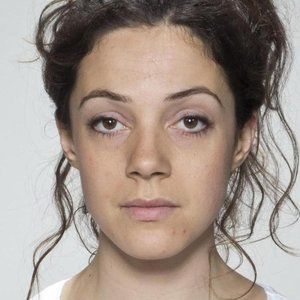
\includegraphics[width=0.125\textwidth]{families_photos/person001_photo.jpg} &
  \frame{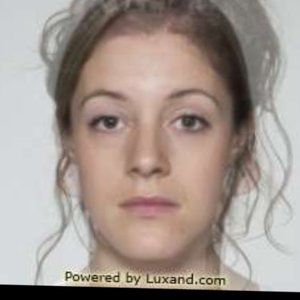
\includegraphics[width=0.125\textwidth]{families_photos/morph_facemorpher.jpg}} &
  \frame{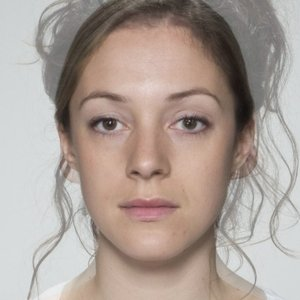
\includegraphics[width=0.125\textwidth]{families_photos/morph_opencv.jpg}} &
  \frame{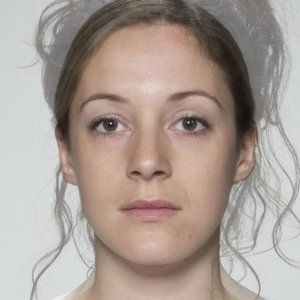
\includegraphics[width=0.125\textwidth]{families_photos/morph_webmorph.jpg}} &
  \frame{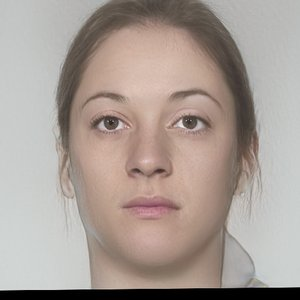
\includegraphics[width=0.125\textwidth]{families_photos/morph_mipgan1.jpg}} &
  \frame{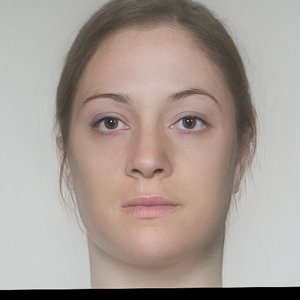
\includegraphics[width=0.125\textwidth]{families_photos/morph_mipgan2.jpg}} &
  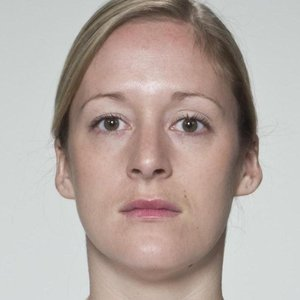
\includegraphics[width=0.125\textwidth]{families_photos/person010_photo.jpg}\\[3pt]
  {\tiny\sffamily\textbf{Source A}} &
  {\tiny\sffamily\textbf{FaceMorpher}} &
  {\tiny\sffamily\textbf{OpenCV}} &
  {\tiny\sffamily\textbf{WebMorph}} &
  {\tiny\sffamily\textbf{MIPGAN-I}} &
  {\tiny\sffamily\textbf{MIPGAN-II}} &
  {\tiny\sffamily\textbf{Source B}}\\[-1pt]
  {\tiny\sffamily contributor 001\_03} &
  \parbox[t]{0.135\textwidth}{\centering\tiny\sffamily halo ring + sharpness/energy} &
  \parbox[t]{0.135\textwidth}{\centering\tiny\sffamily halo + warp-only surround} &
  \parbox[t]{0.135\textwidth}{\centering\tiny\sffamily halo ring + illumination/pose} &
  \parbox[t]{0.135\textwidth}{\centering\tiny\sffamily GAN fingerprint response} &
  \parbox[t]{0.135\textwidth}{\centering\tiny\sffamily GAN fingerprint + sharpness} &
  {\tiny\sffamily contributor 010\_03}\\
\end{tabular}
\caption{Real examples of the five MAD22 morph families analyzed in
Sections~\ref{sec:matched_controls} and~\ref{sec:benchmark_results}. Every morph is a
genuine blend of the same two contributor photographs shown at the ends of
the row (A = 001\_03, B = 010\_03), drawn from the corrected benchmark;
the shortcut label under each panel names the non-identity trait our
instruments isolate for that family. Descriptive illustration only; not a
benchmark claim.}
\label{fig:families_photos}
\end{figure*}



\begin{figure}[tbp]
\centering
% fig:shortcuts_overview -- conceptual taxonomy of non-identity shortcut traits.
% Single-column TikZ (design width 8.2 cm = \columnwidth), native-size fonts,
% no \resizebox, no node-nested \tikz, no \newcommand-pics. Schematic glyphs
% only, no real-face imagery. Suggested include (figure env + caption live in
% main.tex):
%   \begin{figure}[t]\centering% fig:shortcuts_overview -- conceptual taxonomy of non-identity shortcut traits.
% Single-column TikZ (design width 8.2 cm = \columnwidth), native-size fonts,
% no \resizebox, no node-nested \tikz, no \newcommand-pics. Schematic glyphs
% only, no real-face imagery. Suggested include (figure env + caption live in
% main.tex):
%   \begin{figure}[t]\centering% fig:shortcuts_overview -- conceptual taxonomy of non-identity shortcut traits.
% Single-column TikZ (design width 8.2 cm = \columnwidth), native-size fonts,
% no \resizebox, no node-nested \tikz, no \newcommand-pics. Schematic glyphs
% only, no real-face imagery. Suggested include (figure env + caption live in
% main.tex):
%   \begin{figure}[t]\centering\input{figures/shortcuts_overview.tex}...\end{figure}
% Verdicts are the registered reads from results.tex; do not paraphrase stronger.
\centering
\definecolor{tzBlue}{RGB}{47,76,166}
\definecolor{tzOrange}{RGB}{214,116,34}
\definecolor{tzGray}{RGB}{95,100,110}
\definecolor{tzDark}{RGB}{45,50,60}
\begin{tikzpicture}[
  x=1cm,y=1cm,
  font=\sffamily,
  every node/.style={align=left, inner sep=1.5pt, outer sep=0pt},
  fline/.style={line width=1.0pt},
  hrule/.style={draw=tzGray!45, line width=0.6pt},
  boxR/.style={draw=tzBlue, fill=tzBlue!8, rounded corners=3pt, line width=0.8pt},
  fam/.style={draw=tzBlue!60, fill=white, rounded corners=3pt, line width=0.7pt},
  head/.style={anchor=west, font=\sffamily\bfseries\footnotesize, text=tzBlue},
  famHead/.style={anchor=north west, font=\sffamily\bfseries\scriptsize, text=tzDark},
  sub/.style={anchor=north west, font=\sffamily\tiny, text=tzGray},
  trait/.style={anchor=north west, font=\sffamily\tiny, text=tzDark},
  vEst/.style={draw=tzOrange, fill=tzOrange!15, rounded corners=2pt, line width=0.7pt,
               font=\sffamily\tiny, text=tzDark},
  vAtt/.style={draw=tzBlue, fill=tzBlue!8, rounded corners=2pt, line width=0.7pt,
               font=\sffamily\tiny, text=tzDark},
  vInc/.style={draw=tzGray, dashed, fill=tzGray!6, rounded corners=2pt, line width=0.6pt,
               font=\sffamily\tiny, text=tzGray},
  hint/.style={anchor=north west, font=\sffamily\tiny, text=tzGray},
  spoke/.style={->, tzGray!80, line width=0.9pt},
  qlab/.style={font=\sffamily\tiny\itshape, text=tzGray},
]
\useasboundingbox (-0.15,0.05) rectangle (8.35,11.50);

% ============================================================== header
\node[head] at (-0.1,11.28) {What a single-image morph detector can respond to};
\draw[hrule] (-0.05,11.03) -- (8.25,11.03);

% ============================================================== hub node
\draw[boxR] (2.40,7.05) rectangle (5.80,8.00);
\begin{scope}[shift={(3.02,7.52)}]
  \draw[fline, tzBlue] (-0.10,0) circle (0.24);
  \fill[tzBlue] (-0.21,0.07) circle (0.028);
  \fill[tzBlue] (0.01,0.07) circle (0.028);
  \draw[fline, tzBlue] (-0.21,-0.08) arc (215:325:0.13 and 0.09);
  \draw[fline, tzOrange] (0.24,0) circle (0.24);
  \fill[tzOrange] (0.13,0.07) circle (0.028);
  \fill[tzOrange] (0.35,0.07) circle (0.028);
  \draw[fline, tzOrange] (0.13,-0.08) arc (215:325:0.13 and 0.09);
\end{scope}
\node[anchor=west, font=\sffamily\tiny\bfseries, text=tzDark] at (3.55,7.66)
  {morph candidate};
\node[anchor=west, font=\sffamily\tiny, text=tzGray] at (3.55,7.38)
  {single-image (S-MAD) decision};

% ------------------------------------- radiating spokes: hub to trait groups
% top-left
\draw[spoke] (3.05,8.00) -- (2.55,8.36);
% top-right
\draw[spoke] (5.15,8.00) -- (5.65,8.36);
% bottom-left
\draw[spoke] (3.05,7.05) -- (2.55,6.74);
% bottom-right
\draw[spoke] (5.15,7.05) -- (5.65,6.74);
% center: down the corridor between the lower boxes to (5) contributor
\draw[spoke] (4.10,7.05) -- (4.10,3.41);

% ================================================================ 1 TL
\draw[fam] (0.00,8.40) rectangle (3.90,10.78);
\node[famHead] at (0.10,10.73) {(1) Processing \& storage};
\node[sub] at (0.10,10.44) {isolation instruments: MF + CB};
\node[trait] at (0.10,10.16)
  {\textbf{shrink-\&-enlarge history} $256\!\to\!80\!\to\!224$ {\color{tzBlue}\textbf{[MF]}}};
\node[vEst, anchor=north west, text width=3.42cm] at (0.10,9.90)
  {sufficient for 0.0\% EER on native MorDIFF, 10/10 networks, with no morphs in training};
\node[trait] at (0.10,9.16) {\textbf{JPEG / storage size} {\color{tzBlue}\textbf{[MF, CB]}}};
\node[vInc, anchor=north west, text width=3.42cm] at (0.10,8.90)
  {registered combined verdict inconclusive (5/5 trained, 3/5 untrained seeds); false alarms attenuated, not removed};

% ================================================================ 2 TR
\draw[fam] (4.30,8.40) rectangle (8.20,10.78);
\node[famHead] at (4.40,10.73) {(2) Rendering};
\node[sub] at (4.40,10.44) {isolation instrument: MC};
\node[trait] at (4.40,10.16)
  {\textbf{one-photo generative reconstruction} {\color{tzBlue}\textbf{[MC]}}};
\node[vEst, anchor=north west, text width=3.42cm] at (4.40,9.90)
  {render-path verdict \emph{used} (5/5 seeds); 78--90\% of renders flagged despite no second identity};
\node[trait, text width=3.42cm] at (4.40,9.16)
  {\textbf{GAN fingerprints} (MIPGAN, StyleGAN-style) {\color{tzBlue}\textbf{[MC]}}};
\node[vInc, anchor=north west, text width=3.42cm] at (4.40,8.90)
  {inconclusive: low GAN-family EER not established as morph-specific};

% ================================================================ 3 BL
\draw[fam] (0.00,4.25) rectangle (3.90,6.70);
\node[famHead] at (0.10,6.65) {(3) Blending};
\node[sub] at (0.10,6.36) {isolation instrument: MC};
\node[trait, text width=3.42cm] at (0.10,6.08)
  {\textbf{warp geometric trace}, \textbf{tool halo ring},\\[1pt]
   \textbf{noise / variance averaging} {\color{tzBlue}\textbf{[MC]}}};
\node[vInc, anchor=north west, text width=3.42cm] at (0.10,5.44)
  {blend vs warp: $+0.011$ AUC [$-$0.010, 0.031] --- registered: inconclusive};
\node[hint] at (0.10,4.78)
  {low-level statistics: 0.925 / 0.917 AUC (viable)};

% ================================================================ 4 BR
\draw[fam] (4.30,4.25) rectangle (8.20,6.70);
\node[famHead] at (4.40,6.65) {(4) Splice construction};
\node[sub] at (4.40,6.36) {isolation instruments: MC + CB};
\node[trait] at (4.40,6.08) {\textbf{insertion seam} {\color{tzBlue}\textbf{[MC]}}};
\node[vAtt, anchor=north west, text width=3.42cm] at (4.40,5.84)
  {seam-only negative: labels not reproduced from the seam alone};
\node[trait] at (4.40,5.24) {\textbf{same-person splice} {\color{tzBlue}\textbf{[CB]}}};
\node[vAtt, anchor=north west, text width=3.42cm] at (4.40,5.00)
  {flags 70--74\% $\to$ 36--41\% at the own rule: attenuated, still flagged};
\node[vEst, anchor=north west, text width=3.42cm] at (4.40,4.48)
  {full recipe gain $+0.048$ AUC, 5/5 seeds (count-balanced)};

% ================================================================ 5 band
\draw[fam] (0.00,1.95) rectangle (8.20,3.35);
\node[famHead] at (0.10,3.30) {(5) Contributor dependence};
\node[sub] at (3.40,3.30) {isolation instruments: MC + CB};
\node[trait, text width=3.95cm] at (0.10,2.98)
  {a same-person morph blends two photographs of \emph{one} identity:\\[1pt]
   verification helps that person only.};
\node[vInc, anchor=west, text width=3.30cm] at (4.40,2.62)
  {85\% of same-person morphs still flagged --- identity-specific detection: open};

% ============================================================== legend
\node[vEst] at (1.42,1.58) {registered: shortcut used / sufficient};
\node[vAtt] at (3.95,1.58) {attenuated, not removed};
\node[vInc] at (6.62,1.58) {registered: inconclusive / open};
\node[font=\sffamily\tiny, text=tzDark] at (4.10,1.06)
  {\textbf{MF}\, morph-free training\quad
   \textbf{MC}\, matched-control ladder\quad
   \textbf{CB}\, count-balanced training ablation};
\node[qlab] at (4.10,0.52)
  {verdicts are the registered reads of Sec.~4; passing one control does not certify the next};

\end{tikzpicture}
...\end{figure}
% Verdicts are the registered reads from results.tex; do not paraphrase stronger.
\centering
\definecolor{tzBlue}{RGB}{47,76,166}
\definecolor{tzOrange}{RGB}{214,116,34}
\definecolor{tzGray}{RGB}{95,100,110}
\definecolor{tzDark}{RGB}{45,50,60}
\begin{tikzpicture}[
  x=1cm,y=1cm,
  font=\sffamily,
  every node/.style={align=left, inner sep=1.5pt, outer sep=0pt},
  fline/.style={line width=1.0pt},
  hrule/.style={draw=tzGray!45, line width=0.6pt},
  boxR/.style={draw=tzBlue, fill=tzBlue!8, rounded corners=3pt, line width=0.8pt},
  fam/.style={draw=tzBlue!60, fill=white, rounded corners=3pt, line width=0.7pt},
  head/.style={anchor=west, font=\sffamily\bfseries\footnotesize, text=tzBlue},
  famHead/.style={anchor=north west, font=\sffamily\bfseries\scriptsize, text=tzDark},
  sub/.style={anchor=north west, font=\sffamily\tiny, text=tzGray},
  trait/.style={anchor=north west, font=\sffamily\tiny, text=tzDark},
  vEst/.style={draw=tzOrange, fill=tzOrange!15, rounded corners=2pt, line width=0.7pt,
               font=\sffamily\tiny, text=tzDark},
  vAtt/.style={draw=tzBlue, fill=tzBlue!8, rounded corners=2pt, line width=0.7pt,
               font=\sffamily\tiny, text=tzDark},
  vInc/.style={draw=tzGray, dashed, fill=tzGray!6, rounded corners=2pt, line width=0.6pt,
               font=\sffamily\tiny, text=tzGray},
  hint/.style={anchor=north west, font=\sffamily\tiny, text=tzGray},
  spoke/.style={->, tzGray!80, line width=0.9pt},
  qlab/.style={font=\sffamily\tiny\itshape, text=tzGray},
]
\useasboundingbox (-0.15,0.05) rectangle (8.35,11.50);

% ============================================================== header
\node[head] at (-0.1,11.28) {What a single-image morph detector can respond to};
\draw[hrule] (-0.05,11.03) -- (8.25,11.03);

% ============================================================== hub node
\draw[boxR] (2.40,7.05) rectangle (5.80,8.00);
\begin{scope}[shift={(3.02,7.52)}]
  \draw[fline, tzBlue] (-0.10,0) circle (0.24);
  \fill[tzBlue] (-0.21,0.07) circle (0.028);
  \fill[tzBlue] (0.01,0.07) circle (0.028);
  \draw[fline, tzBlue] (-0.21,-0.08) arc (215:325:0.13 and 0.09);
  \draw[fline, tzOrange] (0.24,0) circle (0.24);
  \fill[tzOrange] (0.13,0.07) circle (0.028);
  \fill[tzOrange] (0.35,0.07) circle (0.028);
  \draw[fline, tzOrange] (0.13,-0.08) arc (215:325:0.13 and 0.09);
\end{scope}
\node[anchor=west, font=\sffamily\tiny\bfseries, text=tzDark] at (3.55,7.66)
  {morph candidate};
\node[anchor=west, font=\sffamily\tiny, text=tzGray] at (3.55,7.38)
  {single-image (S-MAD) decision};

% ------------------------------------- radiating spokes: hub to trait groups
% top-left
\draw[spoke] (3.05,8.00) -- (2.55,8.36);
% top-right
\draw[spoke] (5.15,8.00) -- (5.65,8.36);
% bottom-left
\draw[spoke] (3.05,7.05) -- (2.55,6.74);
% bottom-right
\draw[spoke] (5.15,7.05) -- (5.65,6.74);
% center: down the corridor between the lower boxes to (5) contributor
\draw[spoke] (4.10,7.05) -- (4.10,3.41);

% ================================================================ 1 TL
\draw[fam] (0.00,8.40) rectangle (3.90,10.78);
\node[famHead] at (0.10,10.73) {(1) Processing \& storage};
\node[sub] at (0.10,10.44) {isolation instruments: MF + CB};
\node[trait] at (0.10,10.16)
  {\textbf{shrink-\&-enlarge history} $256\!\to\!80\!\to\!224$ {\color{tzBlue}\textbf{[MF]}}};
\node[vEst, anchor=north west, text width=3.42cm] at (0.10,9.90)
  {sufficient for 0.0\% EER on native MorDIFF, 10/10 networks, with no morphs in training};
\node[trait] at (0.10,9.16) {\textbf{JPEG / storage size} {\color{tzBlue}\textbf{[MF, CB]}}};
\node[vInc, anchor=north west, text width=3.42cm] at (0.10,8.90)
  {registered combined verdict inconclusive (5/5 trained, 3/5 untrained seeds); false alarms attenuated, not removed};

% ================================================================ 2 TR
\draw[fam] (4.30,8.40) rectangle (8.20,10.78);
\node[famHead] at (4.40,10.73) {(2) Rendering};
\node[sub] at (4.40,10.44) {isolation instrument: MC};
\node[trait] at (4.40,10.16)
  {\textbf{one-photo generative reconstruction} {\color{tzBlue}\textbf{[MC]}}};
\node[vEst, anchor=north west, text width=3.42cm] at (4.40,9.90)
  {render-path verdict \emph{used} (5/5 seeds); 78--90\% of renders flagged despite no second identity};
\node[trait, text width=3.42cm] at (4.40,9.16)
  {\textbf{GAN fingerprints} (MIPGAN, StyleGAN-style) {\color{tzBlue}\textbf{[MC]}}};
\node[vInc, anchor=north west, text width=3.42cm] at (4.40,8.90)
  {inconclusive: low GAN-family EER not established as morph-specific};

% ================================================================ 3 BL
\draw[fam] (0.00,4.25) rectangle (3.90,6.70);
\node[famHead] at (0.10,6.65) {(3) Blending};
\node[sub] at (0.10,6.36) {isolation instrument: MC};
\node[trait, text width=3.42cm] at (0.10,6.08)
  {\textbf{warp geometric trace}, \textbf{tool halo ring},\\[1pt]
   \textbf{noise / variance averaging} {\color{tzBlue}\textbf{[MC]}}};
\node[vInc, anchor=north west, text width=3.42cm] at (0.10,5.44)
  {blend vs warp: $+0.011$ AUC [$-$0.010, 0.031] --- registered: inconclusive};
\node[hint] at (0.10,4.78)
  {low-level statistics: 0.925 / 0.917 AUC (viable)};

% ================================================================ 4 BR
\draw[fam] (4.30,4.25) rectangle (8.20,6.70);
\node[famHead] at (4.40,6.65) {(4) Splice construction};
\node[sub] at (4.40,6.36) {isolation instruments: MC + CB};
\node[trait] at (4.40,6.08) {\textbf{insertion seam} {\color{tzBlue}\textbf{[MC]}}};
\node[vAtt, anchor=north west, text width=3.42cm] at (4.40,5.84)
  {seam-only negative: labels not reproduced from the seam alone};
\node[trait] at (4.40,5.24) {\textbf{same-person splice} {\color{tzBlue}\textbf{[CB]}}};
\node[vAtt, anchor=north west, text width=3.42cm] at (4.40,5.00)
  {flags 70--74\% $\to$ 36--41\% at the own rule: attenuated, still flagged};
\node[vEst, anchor=north west, text width=3.42cm] at (4.40,4.48)
  {full recipe gain $+0.048$ AUC, 5/5 seeds (count-balanced)};

% ================================================================ 5 band
\draw[fam] (0.00,1.95) rectangle (8.20,3.35);
\node[famHead] at (0.10,3.30) {(5) Contributor dependence};
\node[sub] at (3.40,3.30) {isolation instruments: MC + CB};
\node[trait, text width=3.95cm] at (0.10,2.98)
  {a same-person morph blends two photographs of \emph{one} identity:\\[1pt]
   verification helps that person only.};
\node[vInc, anchor=west, text width=3.30cm] at (4.40,2.62)
  {85\% of same-person morphs still flagged --- identity-specific detection: open};

% ============================================================== legend
\node[vEst] at (1.42,1.58) {registered: shortcut used / sufficient};
\node[vAtt] at (3.95,1.58) {attenuated, not removed};
\node[vInc] at (6.62,1.58) {registered: inconclusive / open};
\node[font=\sffamily\tiny, text=tzDark] at (4.10,1.06)
  {\textbf{MF}\, morph-free training\quad
   \textbf{MC}\, matched-control ladder\quad
   \textbf{CB}\, count-balanced training ablation};
\node[qlab] at (4.10,0.52)
  {verdicts are the registered reads of Sec.~4; passing one control does not certify the next};

\end{tikzpicture}
...\end{figure}
% Verdicts are the registered reads from results.tex; do not paraphrase stronger.
\centering
\definecolor{tzBlue}{RGB}{47,76,166}
\definecolor{tzOrange}{RGB}{214,116,34}
\definecolor{tzGray}{RGB}{95,100,110}
\definecolor{tzDark}{RGB}{45,50,60}
\begin{tikzpicture}[
  x=1cm,y=1cm,
  font=\sffamily,
  every node/.style={align=left, inner sep=1.5pt, outer sep=0pt},
  fline/.style={line width=1.0pt},
  hrule/.style={draw=tzGray!45, line width=0.6pt},
  boxR/.style={draw=tzBlue, fill=tzBlue!8, rounded corners=3pt, line width=0.8pt},
  fam/.style={draw=tzBlue!60, fill=white, rounded corners=3pt, line width=0.7pt},
  head/.style={anchor=west, font=\sffamily\bfseries\footnotesize, text=tzBlue},
  famHead/.style={anchor=north west, font=\sffamily\bfseries\scriptsize, text=tzDark},
  sub/.style={anchor=north west, font=\sffamily\tiny, text=tzGray},
  trait/.style={anchor=north west, font=\sffamily\tiny, text=tzDark},
  vEst/.style={draw=tzOrange, fill=tzOrange!15, rounded corners=2pt, line width=0.7pt,
               font=\sffamily\tiny, text=tzDark},
  vAtt/.style={draw=tzBlue, fill=tzBlue!8, rounded corners=2pt, line width=0.7pt,
               font=\sffamily\tiny, text=tzDark},
  vInc/.style={draw=tzGray, dashed, fill=tzGray!6, rounded corners=2pt, line width=0.6pt,
               font=\sffamily\tiny, text=tzGray},
  hint/.style={anchor=north west, font=\sffamily\tiny, text=tzGray},
  spoke/.style={->, tzGray!80, line width=0.9pt},
  qlab/.style={font=\sffamily\tiny\itshape, text=tzGray},
]
\useasboundingbox (-0.15,0.05) rectangle (8.35,11.50);

% ============================================================== header
\node[head] at (-0.1,11.28) {What a single-image morph detector can respond to};
\draw[hrule] (-0.05,11.03) -- (8.25,11.03);

% ============================================================== hub node
\draw[boxR] (2.40,7.05) rectangle (5.80,8.00);
\begin{scope}[shift={(3.02,7.52)}]
  \draw[fline, tzBlue] (-0.10,0) circle (0.24);
  \fill[tzBlue] (-0.21,0.07) circle (0.028);
  \fill[tzBlue] (0.01,0.07) circle (0.028);
  \draw[fline, tzBlue] (-0.21,-0.08) arc (215:325:0.13 and 0.09);
  \draw[fline, tzOrange] (0.24,0) circle (0.24);
  \fill[tzOrange] (0.13,0.07) circle (0.028);
  \fill[tzOrange] (0.35,0.07) circle (0.028);
  \draw[fline, tzOrange] (0.13,-0.08) arc (215:325:0.13 and 0.09);
\end{scope}
\node[anchor=west, font=\sffamily\tiny\bfseries, text=tzDark] at (3.55,7.66)
  {morph candidate};
\node[anchor=west, font=\sffamily\tiny, text=tzGray] at (3.55,7.38)
  {single-image (S-MAD) decision};

% ------------------------------------- radiating spokes: hub to trait groups
% top-left
\draw[spoke] (3.05,8.00) -- (2.55,8.36);
% top-right
\draw[spoke] (5.15,8.00) -- (5.65,8.36);
% bottom-left
\draw[spoke] (3.05,7.05) -- (2.55,6.74);
% bottom-right
\draw[spoke] (5.15,7.05) -- (5.65,6.74);
% center: down the corridor between the lower boxes to (5) contributor
\draw[spoke] (4.10,7.05) -- (4.10,3.41);

% ================================================================ 1 TL
\draw[fam] (0.00,8.40) rectangle (3.90,10.78);
\node[famHead] at (0.10,10.73) {(1) Processing \& storage};
\node[sub] at (0.10,10.44) {isolation instruments: MF + CB};
\node[trait] at (0.10,10.16)
  {\textbf{shrink-\&-enlarge history} $256\!\to\!80\!\to\!224$ {\color{tzBlue}\textbf{[MF]}}};
\node[vEst, anchor=north west, text width=3.42cm] at (0.10,9.90)
  {sufficient for 0.0\% EER on native MorDIFF, 10/10 networks, with no morphs in training};
\node[trait] at (0.10,9.16) {\textbf{JPEG / storage size} {\color{tzBlue}\textbf{[MF, CB]}}};
\node[vInc, anchor=north west, text width=3.42cm] at (0.10,8.90)
  {registered combined verdict inconclusive (5/5 trained, 3/5 untrained seeds); false alarms attenuated, not removed};

% ================================================================ 2 TR
\draw[fam] (4.30,8.40) rectangle (8.20,10.78);
\node[famHead] at (4.40,10.73) {(2) Rendering};
\node[sub] at (4.40,10.44) {isolation instrument: MC};
\node[trait] at (4.40,10.16)
  {\textbf{one-photo generative reconstruction} {\color{tzBlue}\textbf{[MC]}}};
\node[vEst, anchor=north west, text width=3.42cm] at (4.40,9.90)
  {render-path verdict \emph{used} (5/5 seeds); 78--90\% of renders flagged despite no second identity};
\node[trait, text width=3.42cm] at (4.40,9.16)
  {\textbf{GAN fingerprints} (MIPGAN, StyleGAN-style) {\color{tzBlue}\textbf{[MC]}}};
\node[vInc, anchor=north west, text width=3.42cm] at (4.40,8.90)
  {inconclusive: low GAN-family EER not established as morph-specific};

% ================================================================ 3 BL
\draw[fam] (0.00,4.25) rectangle (3.90,6.70);
\node[famHead] at (0.10,6.65) {(3) Blending};
\node[sub] at (0.10,6.36) {isolation instrument: MC};
\node[trait, text width=3.42cm] at (0.10,6.08)
  {\textbf{warp geometric trace}, \textbf{tool halo ring},\\[1pt]
   \textbf{noise / variance averaging} {\color{tzBlue}\textbf{[MC]}}};
\node[vInc, anchor=north west, text width=3.42cm] at (0.10,5.44)
  {blend vs warp: $+0.011$ AUC [$-$0.010, 0.031] --- registered: inconclusive};
\node[hint] at (0.10,4.78)
  {low-level statistics: 0.925 / 0.917 AUC (viable)};

% ================================================================ 4 BR
\draw[fam] (4.30,4.25) rectangle (8.20,6.70);
\node[famHead] at (4.40,6.65) {(4) Splice construction};
\node[sub] at (4.40,6.36) {isolation instruments: MC + CB};
\node[trait] at (4.40,6.08) {\textbf{insertion seam} {\color{tzBlue}\textbf{[MC]}}};
\node[vAtt, anchor=north west, text width=3.42cm] at (4.40,5.84)
  {seam-only negative: labels not reproduced from the seam alone};
\node[trait] at (4.40,5.24) {\textbf{same-person splice} {\color{tzBlue}\textbf{[CB]}}};
\node[vAtt, anchor=north west, text width=3.42cm] at (4.40,5.00)
  {flags 70--74\% $\to$ 36--41\% at the own rule: attenuated, still flagged};
\node[vEst, anchor=north west, text width=3.42cm] at (4.40,4.48)
  {full recipe gain $+0.048$ AUC, 5/5 seeds (count-balanced)};

% ================================================================ 5 band
\draw[fam] (0.00,1.95) rectangle (8.20,3.35);
\node[famHead] at (0.10,3.30) {(5) Contributor dependence};
\node[sub] at (3.40,3.30) {isolation instruments: MC + CB};
\node[trait, text width=3.95cm] at (0.10,2.98)
  {a same-person morph blends two photographs of \emph{one} identity:\\[1pt]
   verification helps that person only.};
\node[vInc, anchor=west, text width=3.30cm] at (4.40,2.62)
  {85\% of same-person morphs still flagged --- identity-specific detection: open};

% ============================================================== legend
\node[vEst] at (1.42,1.58) {registered: shortcut used / sufficient};
\node[vAtt] at (3.95,1.58) {attenuated, not removed};
\node[vInc] at (6.62,1.58) {registered: inconclusive / open};
\node[font=\sffamily\tiny, text=tzDark] at (4.10,1.06)
  {\textbf{MF}\, morph-free training\quad
   \textbf{MC}\, matched-control ladder\quad
   \textbf{CB}\, count-balanced training ablation};
\node[qlab] at (4.10,0.52)
  {verdicts are the registered reads of Sec.~4; passing one control does not certify the next};

\end{tikzpicture}

\caption{A verdict map of non-identity shortcut traits in single-image morph detection. A morph candidate (center) can be separated from genuine photographs by traits that have nothing to do with combining two identities. The trait groups are those our instruments isolate: processing and storage (morph-free training reaches 0.0\% EER on the native MorDIFF cell), rendering (the render path alone is a registered \emph{used} cue), blending (the matched blend gain is inconclusive), splice construction (matched negatives attenuate, but do not remove, same-person splice flags), and contributor dependence (still open). Each trait carries its isolating instrument: morph-free training (MF), the matched-control ladder (MC), or a count-balanced ablation (CB).}
\label{fig:shortcuts_overview}
\end{figure}


%%%%%%%%%%%


    \begin{table*}[t]
    \centering\small
    \caption{Executed component ablations (CLIP B/16 LoRA, all five seeds 408--412, 6,250 updates, last checkpoints). Recipe flags: W = warp negatives, H = native halves, S = stored-small copies, P = splice positives, N = matched splice negatives ($\times$ = used, empty = not used, p = partial). AUC (S4 vs S3) uses the original development endpoint: it ranks two-person spliced morphs (S4) against stored-small copies (S3), and Flags (\%) is the fraction of stored-small copies flagged at the arm's operating threshold. SbZ/SbH/SbS remove one component from the full recipe Sb (Sp + N) and are not pure one-factor interventions; A/AS is not volume matched.}
    \label{tab:executed_components}
    \begin{tabular}{llccccccrrc}
    \toprule
    Arm & Recipe & W & H & S & P & N & Unique & Rows & AUC (morph vs stored) & Flags on stored (\%) \\
    \midrule
    A & Base: synthetic photos only & & & & & & 1526 & 1992 & 0.559-0.598 & 4.0-7.0 \\
    AS & Base + stored-small (partial) & & & p & & & 2146 & 2850 & 0.577-0.612 & 3.0-5.0 \\
    B & Warp neg. + halves + stored & $\times$ & $\times$ & $\times$ & & & 5099 & 7762 & 0.569-0.601 & 1.0-4.0 \\
    Sp & B + splice positives & $\times$ & $\times$ & $\times$ & $\times$ & & 5223 & 7762 & 0.691-0.722 & 70.0-74.0 \\
    SpV & Sp, repeated native neg. & $\times$ & $\times$ & $\times$ & $\times$ & & 5223 & 8386 & -- & -- \\
    BV & B, repeated native neg. & $\times$ & $\times$ & $\times$ & & & 5099 & 8386 & -- & -- \\
    BN & B + matched neg. & $\times$ & $\times$ & $\times$ & & $\times$ & 5411 & 8386 & -- & -- \\
    Sb & Full: Sp + matched neg. & $\times$ & $\times$ & $\times$ & $\times$ & $\times$ & 5535 & 8386 & 0.755-0.804 & 36.0-41.0 \\
    SbZ & Sb w/o warp negatives & & $\times$ & $\times$ & $\times$ & $\times$ & 4649 & 7868 & 0.754-0.805 & 29.0-41.0 \\
    SbH & Sb w/o native halves & $\times$ & & $\times$ & $\times$ & $\times$ & 3831 & 7200 & 0.773-0.814 & 28.0-32.0 \\
    SbS & Sb w/o stored-small & $\times$ & $\times$ & & $\times$ & $\times$ & 4552 & 8692 & 0.761-0.804 & 33.0-40.0 \\
    \bottomrule
    \end{tabular}
    \par\smallskip\raggedright
    SpV/BV substitute repeated native negatives for 312 matched negatives: counts, classes and positive multisets match within Sb/SpV and BN/BV, but unique-image diversity differs by 312. Their directly paired gains and adverse/null outcomes are in Table~\ref{tab:count_balanced}. Full component hypotheses, per-seed values and storage outcomes remain in the companion appendix.
    \end{table*}

\begin{table}[t]
\centering
\small
\caption{
Count-balanced development comparisons.
Sb and SpV contain identical positive examples,
while Sb replaces repeated ordinary negatives
with 312 additional unique matched negatives.
Intervals use paired component-level bootstrap
resampling conditional on the trained networks.
All five seeds are retained.
}
\label{tab:count_balanced}
\begin{tabular}{@{}p{1.30in}cc@{}}
\toprule
Comparison & $\Delta$AUC & 95\% interval \\
\midrule
\multicolumn{3}{l}{\textit{Whole-frame morphs}} \\
Sb $-$ SpV
    & \textbf{+.0481} & [.0269, .0722] \\
BN $-$ BV
    & $-$.0030 & [$-$.0089, .0045] \\
\midrule
\multicolumn{3}{l}{\textit{Face-spliced morphs}} \\
Sb $-$ SpV
    & \textbf{+.0818} & [.0535, .1083] \\
BN $-$ BV
    & $-$.0247 & [$-$.0455, $-$.0050] \\
\bottomrule
\end{tabular}
\end{table}

\begin{table}[t]
\centering
\small
\caption{
Blend-versus-warp discrimination on the face and
morphing halo. Intervals use host-block bootstrap
resampling over 299 development hosts and condition
on the fitted networks.
}
\label{tab:blend_controls}
\begin{tabular}{lcc}
\toprule
Training & AUC & 95\% interval \\
\midrule
Plain (A)             & 0.864 & [0.848, 0.881] \\
Protocol controls (B) & 0.879 & [0.862, 0.894] \\
Full protocol (Sb)    & 0.889 & [0.873, 0.908] \\
\midrule
Sb $-$ B & +0.011 & [$-$0.010, +0.031] \\
\bottomrule
\end{tabular}
\end{table}



\subsection{Fixed Model and Optimization}
\label{sec:training_implementation}

All primary comparisons use a fixed CLIP ViT-B/16
image encoder~\cite{radford2021clip}, adapted through
low-rank attention updates~\cite{hu2022lora} and a
binary classification head. We use rank-stabilized
LoRA~\cite{kalajdzievski2023rslora} with rank two,
scaling parameter four, and dropout 0.4, applied
to the query and value attention projections.
Normalization parameters remain frozen.

Images are resized to $224 \times 224$ pixels.
Each configuration is trained for 6,250 updates
with batch size 256 using AdamW, weight decay 0.05,
and constant learning rates of
$3.33 \times 10^{-6}$ for the adapted backbone and
$3.33 \times 10^{-5}$ for the classification head.
We use horizontal-flip augmentation and gradient
clipping at five, without label smoothing or
stochastic depth.

Training examples are balanced within source-database
and storage strata by repeating minority-class
examples. Repetitions contribute to training exposure
but are not counted as independent images.
Each primary configuration is evaluated over five
independent training seeds. We use the final checkpoint
without validation-based model selection, and retain
individual network predictions rather than combining
models into an ensemble.
The detector processes a single image at inference.
No source classifier, resolution-dependent decision
rule, or score fusion is introduced. We retain the
original score orientation and report both ranking
metrics and fixed-threshold behavior.
Our experiments therefore assess how changing the
training examples affects a fixed detector, without
confounding the intervention with architectural or
optimization changes.



\end{document}
